\documentclass[a4paper, 12pt]{report}

\title{Конспект лекций по математическому анализу 2023/2024}
\author{Корчагин Егор}
\date { \today }

\usepackage[english, russian]{babel}
\usepackage[T2A]{fontenc}
\usepackage[utf8]{inputenc}
\usepackage{indentfirst}

\usepackage{xr, amsmath, amsfonts, amssymb, amsthm, mathtools, mathtext}

\newtheorem{theorem}{Теорема}[chapter]
\newtheorem{lemma}[theorem]{Лемма}
\newtheorem{mention}[theorem]{Замечание}
\newtheorem{corollary}[theorem]{Следствие}
\newtheorem{definition}[theorem]{Определение}
\newtheorem{example}[theorem]{Пример}
\newtheorem{sentence}[theorem]{Предложение}
\newtheorem*{explanation}{Пояснение}

\usepackage{geometry}
\geometry{top=25mm}
\geometry{bottom=30mm}
\geometry{left=15mm}
\geometry{right=15mm}

\usepackage{titleps}
\newpagestyle{main}{
	\setheadrule{0.4pt}
	\sethead{НИУ ВШЭ}{}{Корчагин Егор}
	\setfootrule{0.4pt}
	\setfoot{Конспект лекций по математическому анализу 2023/2024}{}{\thepage}
}
\pagestyle{main}

\usepackage{soulutf8}

\newcommand{\deriv}[2]{\frac{\partial #1}{\partial #2}}
\newcommand{\R}{\mathbb R}
\newcommand{\Z}{\mathbb Z}
\newcommand{\N}{\mathbb N}
\newcommand{\Q}{\mathbb Q}
\newcommand{\I}{\mathbb I}

\renewcommand{\phi}{\varphi}
\renewcommand{\epsilon}{\varepsilon}
\renewcommand{\kappa}{\varkappa}

\DeclareMathOperator{\Kerr}{Ker}
\DeclareMathOperator{\Imm}{Im}

\DeclareMathOperator*{\argmax}{argmax}

\newcommand{\percent}{\mathbin{\%}}
\newcommand{\symdiff}{\mathbin{\triangle}}



\begin{document}
	
	\maketitle{}
	
	\tableofcontents{}
	
	\large
	
	\chapter{Вещественные числа}
	
	\section*{Лекция 1: Множества, функции, вещественные числа}
	
	\section*{Лекция 2: Множества, функции, вещественные числа}
	
	\chapter{Предел последовательности}
	
	\section*{Лекция 3: Предел числовой последовательности}
	
	\section*{Лекция 4: Теорема Вейерштрасса, число e}
	
	\section*{Лекция 5: Число e, частичный предел}
	
	\section*{Лекция 6: Критерий Коши}
	
	\section*{Лекция 7: Числовые ряды}
	
	\section*{Лекция 8: Перестановка членов ряда}
	
	\chapter{Предел функции}
	
	\section*{Лекция 9: Предел функции}
	
	\section*{Лекция 10: Замечательные пределы, критерий Коши}
	
	\section*{Лекция 11: Эквивалентность и o-символика}
	
	\section*{Лекция 12: Эквивалентность и o-символика}
	
	\section*{Лекция 13: Свойства непрерывных функций}
	
	\chapter{Непрерывные функции}
	
	\section*{Лекция 14: Построение показательной функции}
	
	\chapter{Производная}
	
	\section*{Лекция 15: Производная и дифференциал}
	
	\section*{Лекция 16: Свойства дифференцируемых функций}
	
	\section*{Лекция 17: Теоремы о среднем для дифференцируемых функций}
	
	\section*{Лекция 18: Правило Лопиталя, производные старших порядков}
	
	\section*{Лекция 19: Формула Тейлора}
	
	\section*{Лекция 20: Ряд Тейлора}
	
	\chapter{Исследование функций с помощью производных}
	
	\section*{Лекция 21: Исследование функций с помощью производных}
	
	\section{Необходимое условие экстремума}
	
	Напомним, что для дифференцируемой в точке локального экстремума $c$ функции $f$ по теореме Ферма выполнено $f'(c) = 0$. Т. е. равенство нулю производной является необходимым условием локального экстремума дифференцируемой функции. 
	
	Напомним, что нами также было уже доказано следствие 5.26:
	
	\textbf{Следствие (5.26)} Пусть $f$ дифференцируема в каждой точке интервала $(a, b)$. Тогда $f$ не
	убывает (не возрастает) на $(a, b)$ тогда и только тогда, когда $f'(x) \geqslant 0 \text{ } (f'(x) \leqslant 0$ соответственно) для каждой точки $x \in (a, b)$. Кроме того, если $f'(x) > 0 \text{ } (f'(x) < 0)$, то $f$ строго возрастает (соответственно, строго убывает) на $(a, b)$.
	
	Докажем теперь достаточное условие локального экстремума в терминах производных старших порядков.
	
	\section{Достаточное условие экстремума}

	
	\begin{theorem}
		Пусть $f$ имеет n производных в окрестности точки $c \in (a, b)$ и $f(c) = f'(c) = ... = f^{(n - 1)}(c) = 0$, а $f^{(n)}(c) \neq 0$. Тогда, если $n = 2k$ и $f^{(n)}(c) < 0 \text{ } (f^{(n)}(c) > 0)$, то $c$ — точка локального максимума (минимума). Если $n = 2k + 1$, то точка c не является точкой локального экстремума.
	\end{theorem}
	
	\begin{proof}
		По формуле Тейлора
		\[ f(x) = f(c) + \frac{f'(c)}{1!} \cdot (x - c) + ... + \frac{f^{(n - 1)}(c)}{(n - 1)!}(x - c)^{n - 1} + \frac{f^{(n)}(c)}{n!}(x - c)^n + o((x - c)^n) = \]
		\[ = \frac{f^{(n)}(c)}{n!}(x - c)^n + o((x - c)^n) = (x - c)^n \bigg(\frac{f^{(n)}(c)}{n!} + o(1)\bigg) \]
		Т. к. $o(1) \to 0$ при $x \to c$, то по определению предела
		\[ \exists B_{\delta}(c): \forall x \in B_{\delta}(c) \rightarrow |o(1)| < \epsilon = \bigg|\frac{f^{(n)}{(c)}}{n!}\bigg| \Rightarrow \]
		$\Rightarrow \forall x \in B_{\delta}(c)$ $\big(\frac{f^{(n)}(c)}{n!} + o(1)\big)$ имеет тот же знак, что и $f^{(n)}(c)$
		\begin{enumerate}
			\item Если $n = 2k$ и $f^{(n)}(c) > 0$, то $f(x) = (x - c)^n \big(\frac{f^{(n)}(c)}{n!} + o(1)\big) = (x - c)^{2k} \cdot A(x)$ $(A(x) > 0$ $\forall x \in B_{\delta}(c))$
			
			При $x = c$ $f(c) = 0$; так только мы отходим от точки $c$, $f(x) > 0 \Rightarrow c$ - точка минимума.
			\item Если $n = 2k$ и $f^{(n)}(c) < 0$, то $f(x) = (x - c)^n \big(\frac{f^{(n)}(c)}{n!} + o(1)\big) = (x - c)^{2k} \cdot A(x)$ $(A(x) < 0$ $\forall x \in B_{\delta}(c))$
			
			При $x = c$ $f(c) = 0$; так только мы отходим от точки $c$, $f(x) < 0 \Rightarrow c$ - точка максимума.
			\item Если $n = 2k + 1$ и $f^{(n)}(c) > 0$, то $f(x) = (x - c)^n \big(\frac{f^{(n)}(c)}{n!} + o(1)\big) = (x - c)^{2k + 1} \cdot A(x)$ $(A(x) > 0$ $\forall x \in B_{\delta}(c))$
			
			При $x = c$ $f(c) = 0$; так только мы отходим от точки $c$ в положительную сторону, $f(x) > 0$; так только мы отходим от точки $c$ в отрицательную сторону, $f(x) < 0 \Rightarrow c$ - ни точка максимума, ни точка минимума.
			\item Если $n = 2k + 1$ и $f^{(n)}(c) < 0$, то $f(x) = (x - c)^n \big(\frac{f^{(n)}(c)}{n!} + o(1)\big) = (x - c)^{2k + 1} \cdot A(x)$ $(A(x) < 0$ $\forall x \in B_{\delta}(c))$
			
			При $x = c$ $f(c) = 0$; так только мы отходим от точки $c$ в положительную сторону, $f(x) < 0$; так только мы отходим от точки $c$ в отрицательную сторону, $f(x) > 0 \Rightarrow c$ - ни точка максимума, ни точка минимума.
		\end{enumerate}
		
		Хочется отметить, что выполнение условия теоремы $f(c) = f'(c) = ... = f^{(n - 1)}(c) = 0$ можно гарантировать, сдвинув функцию на константу: $g(x) = f(x) - f(c)$.
	\end{proof}
	
	\section{Выпуклость и вогнутость}
	
	\begin{definition}
		Функция $f$ на интервале $(a, b)$ называется \textbf{выпуклой}, если $\forall x, y \in (a, b)$ и для каждого $t \in [0, 1]$ выполнено
		\[ f(tx + (1 - t)y) \leqslant tf(x) + (1 - t) f(y). \]
	\end{definition}
	
	\begin{explanation}
	    Функция $tx + (1 - t)y$ при фиксированных $x$ и $y$	при различных значениях $t \in [0, 1]$ задаёт точку на отрезке $[x, y]$: при $t = 0$ функция равна $y$, при $t = 1$ функция равна $x$, если возьмём производную функции $tx + (1 - t)y$, то получим $x - y < 0 \Rightarrow$ функция монотонно убывает от $y$ до $x$.
	    
	    Функция $t f(x) + (1 - t) f(y)$ от $t$ является линейной и она задаёт хорду c концами в точках $(x, f(x))$ (при $t = 1$) и $(y, f(y))$ (при $t = 0$). 
	    
	    Получается с левой стороны неравенства - это значение функции в точке на отрезке $[x, y]$, а с правой - ордината точки на хорде и понятно, что неравенство выполняется.
	\end{explanation}
	
	\begin{center}
		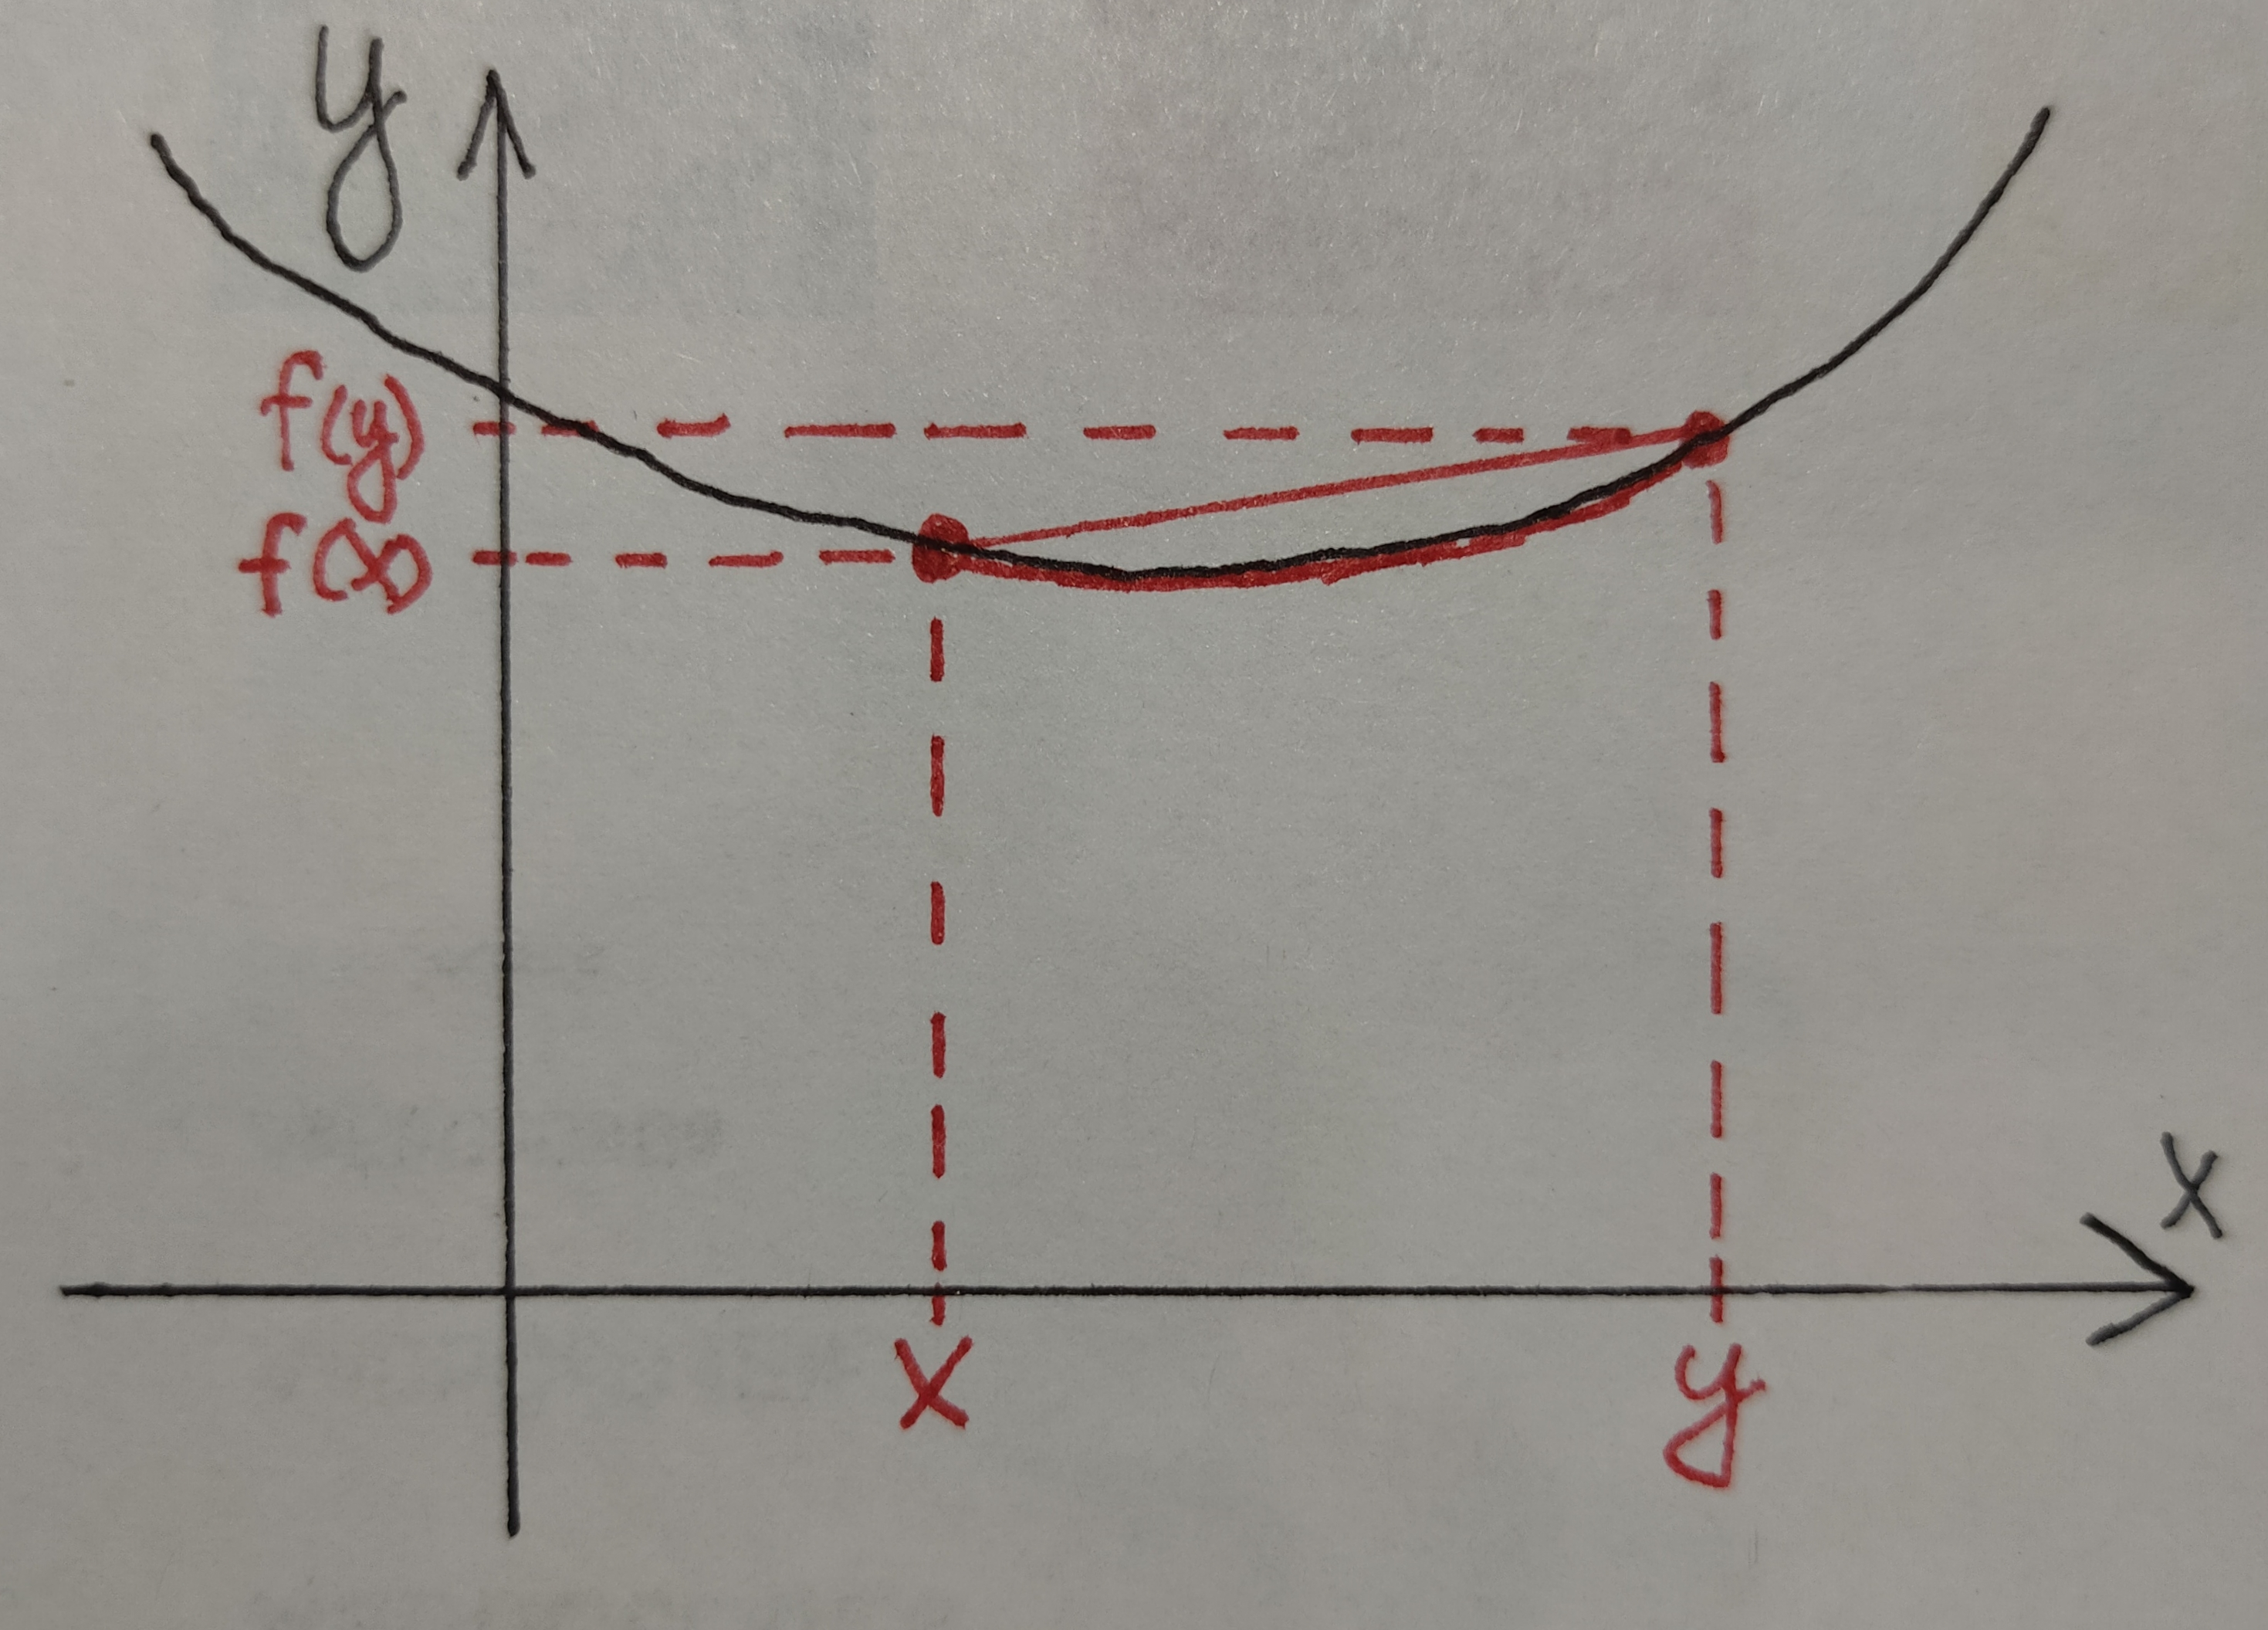
\includegraphics[width=0.4\textwidth]{img/lecture21/convex}
	\end{center}
	
	
	\begin{definition}
		Функция $f$ на интервале $(a, b)$ называется \textbf{вогнутой}, если $\forall x, y \in (a, b)$ и для каждого $t \in [0, 1]$ выполнено
		\[ f(tx + (1 - t)y) \geqslant tf(x) + (1 - t)f(y). \]
	\end{definition}
	
	
	\begin{lemma}
		Функция $f$ на интервале $(a, b)$ выпукла тогда и только тогда, когда для всех точек $x < z < y$ из этого интервала выполнено
		\[ \frac{f(z) - f(x)}{z - x} \leqslant \frac{f(y) - f(z)}{y - z} \]
	\end{lemma}
	
	\begin{proof}
		Неравенство, которое нужно доказать эквивалентно
		\[ \frac{f(z) - f(x)}{z - x} \leqslant \frac{f(y) - f(z)}{y - z} \text{ } \bigg| \cdot (z - x)(y - z) \]
		\[ yf(z) - zf(z) - yf(x) + zf(x) \leqslant zf(y) - xf(y) - zf(z) + xf(z) \]
		\[ xf(z) - yf(z) \geqslant zf(x) - yf(x) + xf(y) - zf(y) \]
		
		Т. к. $x < z < y$, то $\exists t \in [0, 1]$ $z = t \cdot x + (1 - t) \cdot y \Leftrightarrow t = \frac{z - y}{x - y}$.
		
		Т. к. $f(x)$ - выпукла, то $f(z) = f(t \cdot x + (1 - t) \cdot y) \leqslant t f(x) + (1 - t) f(y) = \frac{z - y}{x - y} f(x) + \frac{x - z}{x - y} f(y) \Leftrightarrow xf(z) - yf(z) \geqslant zf(x) - yf(x) + xf(y) - zf(y)$, т. е пришли к тому же самому неравенству.
		
		В обратную сторону.	Имеем, что
		\[ \frac{f(z) - f(x)}{z - x} \leqslant \frac{f(y) - f(z)}{y - z} \Rightarrow xf(z) - yf(z) \geqslant zf(x) - yf(x) + xf(y) - zf(y) \Rightarrow \]
		\[ \Rightarrow f(z) \leqslant \frac{z - y}{x - y} f(x) + \frac{x - z}{x - y} f(y) \]
		Т. к. $x < z < y$, то $\exists t \in [0, 1]$ $z = t \cdot x + (1 - t) \cdot y \Leftrightarrow t = \frac{z - y}{x - y}$.
		
		Значит
		\[  f(t \cdot x + (1 - t) \cdot y) \leqslant t f(x) + (1 - t) f(y), \]
		что является определением выпуклости функции.
	\end{proof}
	
	\begin{theorem}
		Дифференцируемая функция $f$ на интервале $(a, b)$ выпукла тогда и только тогда, когда $f'$ — неубывает.
	\end{theorem}
	
	\begin{proof}
		\begin{enumerate}
			\item[$\Rightarrow$] $\forall x < z < y \in (a, b)$
			$f$ - выпукла $\Rightarrow$ по предыдущей лемме
			\[ \frac{f(z) - f(x)}{z - x} \leqslant \frac{f(y) - f(z)}{y - z} \]
			Тогда при $z \to x$ по теореме о переходе к пределу в неравенстве
			\[ f'(x) \leqslant \frac{f(y) - f(x)}{y - x} \]
			(Здесь есть тонкость: мы можем устремлять $z$ к $x$ только справа, поэтому мы получим правую производную, но если функция дифференцируема, то правая производная совпадает с левой)
			
			Пусть $z \to y$. Тогда
			\[ \frac{f(y) - f(x)}{y - x} \leqslant f'(y) \]
		    Таким образом, $\forall x < y$ $f'(x) \leqslant f'(y) \Rightarrow f'(x)$ - неубывает. 
			\item[$\Leftarrow$] Пусть $x < z < y$
			
			По теореме Лагранжа $\exists \xi_1 \in (x, z): \frac{f(z) - f(x)}{z - x} = f'(\xi_1)$
			
			$\exists \xi_2 \in (z, y): \frac{f(y) - f(z)}{y - z} = f'(\xi_2)$
			
			Таким образом, $\xi_1 \leqslant \xi_2 \Rightarrow f'(\xi_1) \leqslant f'(\xi_2) \Rightarrow \frac{f(z) - f(x)}{z - x} \leqslant \frac{f(y) - f(z)}{y - z} \Rightarrow f$ на интервале $(a, b)$ выпукла по предыдущей лемме.
		\end{enumerate}
	\end{proof}
	
	\begin{corollary}
		Дважды дифференцируемая функция $f$ на интервале $(a, b)$ выпукла тогда и только тогда, когда $f''(x) \geqslant 0 \text{ } \forall x \in (a, b).$
	\end{corollary}
	
	\begin{proof}
		$f''(x) \geqslant 0 \Leftrightarrow f'(x)$ неубывает. 
	\end{proof}
	
	\begin{corollary}
		Пусть $f$ — дифференцируемая выпуклая функция на интервале $(a, b)$. Тогда $f(x) \geqslant f'(c)(x - c) + f(c)$ для всех $x, c \in (a, b)$.
    \end{corollary}
    
    \begin{proof}
    	$f(x) \geqslant f'(c)(x - c) + f(c) \Leftrightarrow f(x) - f(c) \geqslant f'(c)(x - c) \text{ } (*)$
    	\begin{enumerate}
    		\item Пусть $x > c$
    		\[ (*) \Leftrightarrow \frac{f(x) - f(c)}{x - c} \geqslant f'(c) \]
    		По теореме Лагранжа $\exists \xi \in (c, x) :$
    		\[ \frac{f(x) - f(c)}{x - c} = f'(\xi) \geqslant f'(c), \]
    		т. к. функция выпукла и по теореме 6.5 и функция неубывает.
    		\item Пусть $x < c$
    		\[ (*) \Leftrightarrow \frac{f(x) - f(c)}{x - c} \leqslant f'(c) \]
    		По теореме Лагранжа $\exists \xi \in (x, c) :$
    		\[ \frac{f(x) - f(c)}{x - c} = f'(\xi) \leqslant f'(c), \]
    		т. к. функция выпукла и по теореме 6.5 и функция неубывает.
    		\item Пусть $x = c$. Тогда $(*): 0 \geqslant 0$.
    	\end{enumerate}
    \end{proof}
    
    \section{Неравенство Йенсена}
    
    \begin{theorem}[Неравенство Йенсена]
    	Пусть функция $f$ выпукла на интервале $(a, b)$. Тогда для всех $x_1, ..., x_n \in (a, b)$ и для всех чисел $t_1 \geqslant 0, ..., t_n \geqslant 0$, для
    	которых $t_1 + ... + t_n = 1$, выполнено
    	\[ f(t_1 x_1 + ... + t_n x_n) \leqslant t_1 f(x_1) + ... + t_n f(x_n). \]
    \end{theorem}
    
    \begin{proof}
    	Индукция по $n$. База индукции: $n = 2$
    	\[ t_1 + t_2 = 1 \Rightarrow t_2 = 1 - t_1 \Rightarrow \]
    	\[ \Rightarrow f(t_1 x_1 + t_2 x_2) = f(t_1 x_1 + (1 - t_1) x_2) \leqslant t_1 f(x_1) + (1 - t_1) f(x_2) = t_1 f(x_1) + t_2 f(x_2) \]
    	по определению выпуклости.
    	
    	Шаг индукции: пусть $t_1 + ... + t_n + t_{n + 1} = 1$. Возьмём $t = t_1 + ... + t_n \Rightarrow t + t_{n + 1} = 1$
    	\[ f(t_1 x_1 + ... + t_n x_n + t_{n + 1} x_{n + 1}) = f\bigg(t\bigg(\frac{t_1}{t} x_1 + ... + \frac{t_n}{t} x_n\bigg) + t_{n + 1} x_{n + 1}\bigg) = (*) \]
    	Тогда из выпуклости функции
    	\[ (*) \leqslant t f\bigg(\frac{t_1}{t} f(x_1) + ... + \frac{t_n}{t} f(x_n)\bigg) + t_{n + 1} f(x_{n + 1}) = (**)  \]
    	$\frac{t_1}{t} + ... + \frac{t_n}{t} = \frac{t_1 + ... + t_n}{t} = \frac{t}{t} = 1$. Применяем предположение индукции
    	\[ (**) \leqslant t\bigg(\frac{t_1}{t} f(x_1) + ... + \frac{t_n}{t} f(n)\bigg) + t_{n + 1} f(x_{n + 1}) = t_1 f(x_1) + ... + t_n f(n) + t_{n + 1} f(x_{n + 1}) \]
    \end{proof}
    
    \begin{example}[Неравенство о средних]
    	Пусть $x_1, ..., x_n > 0$. Тогда $\sqrt[n]{x_1 ... x_n} \leqslant \frac{x_1 + ... + x_n}{n}$.
    \end{example}
    
    $t_1 = t_2 = ... = t_n = \frac{1}{n}, f(x) = e^x, y_i = \ln{x_i}$
    
    $f''(x) = e^x \geqslant 0 \text{ } \forall x \Rightarrow f(x) = e^x$ - выпуклая.
    
    По неравенству Йенсена
    \[ f(t_1 y_1 + ... + t_n y_n) \leqslant t_1 f(y_1) + ... + t_n f(y_n) \]
    \[ f(t_1 y_1 + ... + t_n y_n) = e^{t_1 y_1 + ... + t_n y_n} = e^{\frac{\ln{x_1}}{n} + \frac{\ln{x_2}}{n} + ... + \frac{\ln{x_n}}{n}} = e^{\frac{\ln{x_1}}{n}} \cdot ... \cdot e^{\frac{\ln{x_n}}{n}} = \sqrt[n]{x_1 ... x_n} \]
    \[ t_1 f(y_1) + ... + t_n f(y_n) = \frac{1}{n} (x_1 + ... + x_n) \]
    
    \section{Асимптоты}
    
    \begin{definition}
    	Прямая $y = \alpha x + \beta$ называется \textbf{асимптотой} графика функции
    	$f$ при $x \to +\infty$ $(x \to -\infty)$, если $f(x) = \alpha x + \beta + o(1)$ при
    	$x \to +\infty$ $(x \to -\infty)$. Ясно, что в случае асимптоты на $+\infty$
    	справедливы равенства
    	\[ \alpha = \lim_{x \to +\infty} \frac{f(x)}{x}, \beta = \lim_{x \to +\infty} (f(x) - \alpha x) \]
    	Аналогичные равенства верны и в случае асимптоты на $-\infty$ с
    	заменой везде $+\infty$ на $-\infty$.
    \end{definition}
	
	\chapter{Первообразная и неопределенный интеграл}
	
	\section*{Лекция 22: Первообразная, неопределённый интеграл}
	
	\section{Первообразная}
	
	\begin{definition}
		Функция $F$ называется первообразной функции $f$ на некотором интервале $I$, если $F$ дифференцируема на $I$ и $F'(x) = f(x)$ $\forall x \in I$.
	\end{definition}
	
	\underline{Педагогический приём.}
	$\frac{1}{x} = (\ln{|x|})' = \frac{2}{2x} = (\ln{|2x|})'$, т. к. $\ln{2x} = \ln{2} + \ln{x}$, т. е. отличается на константу.
	
	\begin{lemma}
		Любые две первообразные $F_1$ и $F_2$ функции $f$ на интервале $I$ отличаются на константу.
	\end{lemma}
	
	\begin{proof}
		Ф$(x) = F_1(x) - F_2(x)$
		
		Ф$(x)$ дифференцируема как сумма дифференцируемых функций.
		
		Ф$'(x) = (F_1(x) - F_2(x))' = f(x) - f(x) = 0$
		
		Т. к. Ф$(x)$ дифференцируема $\Rightarrow$ непрерывна на любом интервале.
		
		По теореме Лангранжа 
		
		$\forall a, b \in I, a \leqslant b$ $\exists c \in (a, b) \rightarrow$ Ф$(a)$ - Ф$(b) = $ Ф$'(c)(a - b) = 0 \cdot (a - b) = 0.$ Значит Ф$(x) = const$.
	\end{proof}
	
	\begin{definition}
		Множество всех первообразных функции $f$ на некотором заданном интервале $I$ называется \underline{неопределённым интегралом} от $f$ и обозначается $\displaystyle\int f(x) \; dx$.
	\end{definition}
	
	$\displaystyle\int f(x) \; dx = \{F(x) + C$ | $F(x)$ - первообразная $f(x), C \in \R\}$
	
	\section{Таблица первообразных}
	\begin{itemize}
		\item $\displaystyle\int x^a \; dx = \frac{x^{a + 1}}{a + 1} + C, a \neq -1;$
		\item $\displaystyle\int \frac{dx}{x} \; dx = \ln{|x|} + C;$
		\item $\displaystyle\int e^x \; dx = e^x + C;$
		\item $\displaystyle\int \sin{x} \; dx = -\cos{x} + C;$
		\item $\displaystyle\int \cos{x} \; dx = \sin{x} + C;$
		\item $\displaystyle\int \frac{dx}{\cos^2{x}} = \tg{x} + C;$
		\item $\displaystyle\int \frac{dx}{\sin^2{x}} = -\ctg{x} + C;$
		\item $\displaystyle\int \frac{dx}{1 + x^2} = \arctg{x} + C;$
		\item $\displaystyle\int \frac{dx}{\sqrt{1 - x^2}} = \arcsin{x} + C;$
	\end{itemize}
	
	\section{Свойства неопределённого интеграла}
	
	\begin{theorem}
		\begin{enumerate}
			\item (Линейность) 
			
			\[\int \alpha f(x) + \beta g(x) \; dx = \alpha \int f(x) \; dx + \beta \int g(x) \; dx + C;\]
			
			\item (Формула интегрирования по частям) 
			
			\[\int f(x)g'(x) \; dx = f(x)g(x) - \int f'(x)g(x) \; dx;\]
			
			\item (Формула замены переменной)
			
			\[\int f(\phi(t))\phi'(t) \; dt = \int f(x) \; dx\bigg|_{x=\phi(t)}.\]
			
		\end{enumerate}
		
	    (Здесь подразумевается, что все интегралы существуют.)
	\end{theorem}
	
	\begin{proof}
		\begin{enumerate}
			\item Пусть $F'(x) = f(x), G'(x) = g(x).$
			
			$(\alpha F(x) + \beta G(x))' = \alpha F'(x) + \beta G'(x) = \alpha f(x) + \beta g(x) \Rightarrow \alpha F(x) + \beta G(x)$ - первообразная функции $\alpha f(x) + \beta g(x) \Rightarrow \displaystyle\int \alpha f(x) + \beta g(x) \; dx = \alpha F(x) + \beta G(x) + C$.
					
			А также $\alpha \displaystyle\int f(x) \; dx + \beta \displaystyle\int g(x) \; dx = \alpha F(x) + \alpha c_1 + \beta G(x) + \beta c_2 = \alpha F(x) + \beta G(x) + C$.
			
			\item $(f(x)g(x))' = f'(x)g(x) + f(x)g'(x) \Rightarrow f(x)g(x) + C =$
			
			$=\displaystyle\int f'(x)g(x) + f(x)g'(x) \; dx = \displaystyle\int f'(x)g(x) \; dx + \displaystyle\int f(x)g'(x) \; dx$ (линейность)
			
			$\Rightarrow \displaystyle\int f(x)g'(x) = f(x)g(x) - \displaystyle\int f'(x)g(x) \; dx$.
			
			\item $(F(\phi(t)))'_t = F'_x(\phi(t))\phi'(t) = f(\phi(t))\phi'(t) \Rightarrow F(\phi(t)) \in \displaystyle\int f(\phi(t))\phi'(t)dt$.
			
			С другой стороны, $F(\phi(t)) \in \displaystyle\int f(x) \; dx \bigg|_{x=\phi(t)}$.
			
			Следовательно, $\displaystyle\int f(\phi(t))\phi'(t) \; dt = \displaystyle\int f(x) \; dx\bigg|_{x=\phi(t)}$.
		\end{enumerate}		
    \end{proof}
    
    \begin{mention}
    	Отметим, что, т.к. $f'(x) \; dx = df$ и $g'(x) \; dx = dg$ (инвариантность первого дифференциала), то свойство 2) обычно записывают в виде $\displaystyle\int f \; dg = fg - \displaystyle\int g \; df$.
    	
    	Аналогично, свойство 3) обычно записывают в виде $\displaystyle\int f(\phi(t))\phi'(t) \; dt =$    	
    	
    	$= \displaystyle\int f(\phi(t)) \; d\phi(t)$ и рассматривают $\phi$ как новую переменную.
    \end{mention}
    
    \begin{example} Найдём следующие первообразные:
    
    \begin{enumerate}
    	\item[1.1] $\displaystyle\int \cos^9{x} \sin{x} \; dx = -\displaystyle\int \cos^9{x} (\cos{x})' \; dx =$ (формула замены переменной) $-\displaystyle\int t^9 \; dt\bigg|_{t=\cos{x}} = -\frac{t^{10}}{10} + C\bigg|_{t=\cos{x}} = -\frac{\cos^{10}{x}}{10} + C$;
    		
    	\item[1.2] $\displaystyle\int \cos^9{x} \sin{x} \; dx = -\displaystyle\int \cos^9{x} (\cos{x})' \; dx =$ (Замечание 7.6) $ -\displaystyle\int \cos^9{x} \;  d\cos{x} = -\frac{\cos^{10}{x}}{10} + C$;
    		
    	Здесь $\cos{x}$ воспринимаем как переменную.
    	
    	\item[2.1] $\displaystyle\int \ln{x} \; dx = \displaystyle\int \ln{x} \cdot 1 \; dx = \displaystyle\int \ln{x} \cdot x' \; dx =$ (формула интегрирования по частям) $x\ln{x} - \displaystyle\int x(\ln{x})' \; dx = x\ln{x} - \displaystyle\int 1 \; dx = x\ln{x} - x + C$;
    		
    	\item[2.2] $\displaystyle\int \ln{x} \; dx = x\ln{x} - \displaystyle\int x \; d\ln{x} = x\ln{x} - \displaystyle\int x \cdot \frac{1}{x} \; dx = x\ln{x} - x + C$;
    	
    	\item[3.] $\displaystyle\int \sqrt{1 - x^2} \; dx = \bigg[x = \cos{t}; -1 \leqslant x \leqslant 1; t = \arccos{x}; 0 \leqslant t \leqslant \pi \bigg]$ (здесь используем формулу замены переменной в обратную сторону) 
    	
    	$= \displaystyle\int \sqrt{1 - \cos^2{t}} \; d\cos{t} = -\displaystyle\int \sqrt{1 - \cos^2{t}} \sin{t} \; dt = -\displaystyle\int \sin^2{t} \; dt$ $(t \geqslant 0)$ $= -\displaystyle\int 1 - \cos^2{t} \; dt = \displaystyle\int \cos^2{t} - 1 \; dt = \displaystyle\int \cos^2{t} \; dt - \displaystyle\int 1 \; dt = \displaystyle\int \frac{1 + \cos{2x}}{2} \; dt - t = \displaystyle\int \frac{1}{2} \; dt + \frac{1}{2} \displaystyle\int \cos{2t} \; dt - t = \frac{1}{2}t + \frac{1}{2}\frac{\sin{2t}}{2} + C = \frac{1}{2}t + \frac{1}{2}\sin{t}\cos{t} + C = \frac{1}{2}\arccos{x} + \frac{1}{2}\cos{(\arccos{x})}\sin{(\arccos{x})} + C$ (мы подставили в $\phi(t)$ $t = \phi^{-1}(x)$ и получили, что $\phi(\phi^{-1}(x)) = x$, т. к. $\phi(t) = \cos{t}$ - биекция) $= \frac{1}{2}\arccos{x} + \frac{1}{2}x\sqrt{1 - x^2} + C;$
    	
    \end{enumerate}
    \end{example}
      
    Как мы поняли, интеграл - это обратная операция к дифференцированию и обратные операции часто усторены сложнее, чем прямые. Так и с интегралом: если продифференцировать можно почти любую функцию в виде формулы, то интеграл от функции, выраженной через элементарные функции, иногда не может быть выражен через элементарные функции. Но для некоторых функций ответ выражается через элементарные. В частности, всегда можно найти интеграл от рациональной функции, но с некоторой оговоркой.
	
	\chapter{Интеграл от рациональной функции}
	
	\section*{Лекция 23: Интеграл от рациональной функции}
	
	\section{Рациональная функция}
	
	\begin{definition}
		Функция $R(x)$ называется \underline{рациональной}, если 
		
		\[R(x) = \frac{P(x)}{Q(x)}\]
		
		для некоторых многочленов P(x) и Q(x).
	\end{definition}
	
	\begin{example} Найдём следующие первообразные:
	
	\begin{enumerate}
		\item $\displaystyle\int \frac{1}{x(x - 1)} \; dx = \displaystyle\int \bigg(\frac{1}{x - 1} - \frac{1}{x} \bigg) \; dx = \displaystyle\int \frac{1}{x - 1} \; dx - \displaystyle\int \frac{1}{x} \; dx = \ln{|x - 1|} - \ln{|x|} + C$;
		
		\item $\displaystyle\int \frac{1}{x(x - 1)^2} \; dx = \displaystyle\int \frac{1}{x - 1}\frac{1}{x(x - 1)} \; dx = \displaystyle\int \frac{1}{x - 1}\bigg(\frac{1}{x - 1} - \frac{1}{x} \bigg) \; dx = \displaystyle\int \frac{1}{(x - 1)^2} - \frac{1}{x(x - 1)} \; dx = \displaystyle\int \frac{1}{(x - 1)^2} \; dx - \displaystyle\int \frac{1}{x(x - 1)} \; dx = \displaystyle\int \frac{1}{(x - 1)^2} \; dx - \displaystyle\int \frac{1}{x - 1} \; dx + \displaystyle\int \frac{1}{x} \; dx$ (используем пункт 1) $= -\frac{1}{x - 1} - \ln{|x - 1|} + \ln{|x|} + C$;
		
		\item $\displaystyle\int \frac{1}{x(x^2 + 1)} \; dx = \displaystyle\int \frac{1}{x} - \frac{x}{x^2 + 1} \; dx = \displaystyle\int \frac{1}{x} \; dx - \displaystyle\int \frac{x}{x^2 + 1} \; dx = \ln{|x|} + C - \frac{1}{2}\displaystyle\int \frac{2x}{x^2 + 1} \; dx = \ln{|x|} + C - \frac{1}{2}\displaystyle\int \frac{d(x^2 + 1)}{x^2 + 1}$ $(d(x^2 + 1) = (x^2 + 1)'dx = 2xdx)$ $= \ln{|x|} - \frac{1}{2}\ln{|x^2 + 1|} + C$;
		
	\end{enumerate}
	\end{example}
	
	\section{Разложение многочлена на неприводимые}
	
	\begin{theorem}
		Любой многочлен единственным образом раскладывается на неприводимые множители. (без доказательства)
	\end{theorem}
	
	\begin{mention}
		Любой многочлен $P(x) \in \R[x]$ раскладывается на множители вида $(x - a)$ и $(x^2 + px + q)$, где $p^2 - 4q < 0$ (дискриминант меньше нуля).	
	\end{mention}
	
	\section{Правильная дробь}
	
	\begin{definition}
		Рациональная дробь $\frac{P(x)}{Q(x)}$
		\underline{правильная}, если степень числителя
		меньше степени знаменателя. Нулевой многочлен 0 является правильной дробью.
	\end{definition}
	
	\begin{mention}
		Любая рациональная дробь единственным способом
		представима как сумма многочлена и правильной дроби.
	\end{mention}
	
	\section{Элементарная дробь}
	
	\begin{definition}
		Правильная рациональная дробь $\frac{P(x)}{Q(x)}$ называется \underline{элементарной} \underline{(или простейшей)}, если её знаменатель $Q(x)$ представляет собой степень неприводимого многочлена $p(x)$:
		\[ Q(x) = p^k(x), k \leqslant 1, \]
		а степень числителя $P(x)$ меньше степени $p(x)$.
	\end{definition}
	
	\section{Разложение дроби на элементарные}
	
	\begin{theorem}
		Любая правильная рациональная дробь единственным образом разлагается в сумму элементарных дробей. (без доказательства)
	\end{theorem}
	
	\begin{corollary}
		Каждая рациональная функция $\frac{P(x)}{Q(x)}, P(x), Q(x) \in \R[x]$
		представима в виде суммы многочлена и элементарных рациональных дробей
		\[\frac{A}{(x - a)^m}, \frac{Mx + N}{(x^2 + px + q)^n}, p^2 - 4q < 0, A, M, N \in \R.\]
	\end{corollary}
	
	\section{Интегрирование рациональных функций}
	
	\begin{theorem}
		Пусть $P$ и $Q$ два многочлена. Тогда первообразная функции $\frac{P}{Q}$ выражается в элементарных функциях (более точно, рациональных, $ln$ и $arctg$).
	\end{theorem}
	
	\begin{proof}
		Пусть $Q(x) = (x - a_1)^{m_1} \cdot ... \cdot (x - a_s)^{m_s} \cdot (x^2 + p_1x + q_1)^{n_1} \cdot ... \cdot (x^2 + p_kx + q_k)^{n_k}.$ По теореме 8.8 дробь $\frac{P(x)}{Q(x)}$ раскладывается в сумму элементарных дробей
		\[\frac{P(x)}{Q(x)} = R(x) + \sum_{i = 1}^{s} \sum_{j = 1}^{m_i} \frac{A_{ij}}{(x - a_i)^j} + \sum_{i = 1}^{k} \sum_{j = 1}^{n_i} \frac{B_{ij}x + C_{ij}}{(x^2 + p_ix + q_i)^j}.\]
		(Здесь более сильное утверждение: любая рациональная функция раскладывается в виде суммы \textit{именно таких} элементарных дробей)
		
		Чтобы проинтегрировать $\frac{P(x)}{Q(x)}$, нужно, в силу линейности интеграла, проинтегрировать по отдельности многочлен $R(x)$ и элементарные дроби. Но многочлен мы уже умеем интегрировать, осталось разобраться с элементарными дробями.
		
		\begin{enumerate}
			\item $\displaystyle\int \frac{Adx}{x - a} = A ln{|x - a| + C}$;
			\item $\displaystyle\int \frac{Adx}{(x - a)^n} = - \frac{A}{(n - 1)(x - a)^{n - 1}} + C, n \neq 1$ (проверяется взятием производной у правой части);
			\item Воспользуемся тем, что $\displaystyle\int \frac{1}{x^2 + a^2} \; dx = \frac{1}{a^2} \displaystyle\int \frac{dx}{(\frac{x}{a})^2 + 1} = \frac{1}{a} \displaystyle\int \frac{d\frac{x}{a}}{(\frac{x}{a})^2 + 1} = \frac{1}{a} \arctg{(\frac{x}{a})} + C.$
			
			$\displaystyle\int \frac{Mx + N}{x^2 + px + q} \; dx = M \displaystyle\int \frac{x + \frac{N}{M}}{x^2 + px + q} \; dx = \frac{M}{2} \displaystyle\int \frac{2x + p - p + \frac{2N}{M}}{x^2 + px + q} \; dx = \frac{M}{2} \displaystyle\int \frac{2x + p}{x^2 + px + q} \; dx + \frac{M}{2} \displaystyle\int \frac{\frac{2N}{M} - p}{x^2 + px + q} \; dx = \frac{M}{2} \displaystyle\int \frac{d(x^2 + px + q)}{x^2 + px + q} \; dx + \frac{M}{2} \bigg(\frac{2N}{M} - p\bigg) \displaystyle\int \frac{dx}{(x + \frac{p}{2})^2 + q - \frac{p^2}{4}} = \frac{M}{2} \ln{(x^2 + px + q)} +$ 
			
			$\bigg(N - \frac{pM}{2}\bigg)\frac{1}{\sqrt{q - \frac{p^2}{4}}}\arctg{\frac{x + \frac{p}{2}}{\sqrt{q - \frac{p^2}{4}}}} + C$ ($x^2 + px + q > 0$, т. к. $D = p^2 - 4q < 0$, ещё здесь пользуемся верхним интегралом);
			
			\item $n \in \N, a \neq 0, J_n(x, a) = \displaystyle\int \frac{dx}{(x^2 + a^2)^n} = \frac{x}{(x^2 + a^2)^n} - \displaystyle\int x d\bigg(\frac{1}{(x^2 + a^2)^n}\bigg)$ (формула интегрирования по частям) $= \frac{x}{(x^2 + a^2)^n} + \displaystyle\int \frac{x \cdot n \cdot 2x}{(x^2 + a^2)^{n + 1}} \; dx = \frac{x}{(x^2 + a^2)^n} + 2n \displaystyle\int \frac{x^2}{(x^2 + a^2)^{n + 1}} \; dx = \frac{x}{(x^2 + a^2)^n} + 2n \displaystyle\int \frac{x^2 + a^2 - a^2}{(x^2 + a^2)^{n + 1}} \; dx = \frac{x}{(x^2 + a^2)^n} + 2n \displaystyle\int \frac{x^2 + a^2}{(x^2 + a^2)^{n + 1}} \; dx - 2n \displaystyle\int \frac{a^2}{(x^2 + a^2)^{n + 1}} \; dx = \frac{x}{(x^2 + a^2)^n} + 2n J_n(x, a) - 2na^2 J_{n + 1}(x, a) \Rightarrow J_{n + 1}(x, a) = \frac{1}{2na^2} \bigg(\frac{x}{(x^2 + a^2)^n} + 2nJ_n(x, a) - J_n(x, a)\bigg)$ $= \frac{1}{2na^2} \bigg(\frac{x}{(x^2 + a^2)^n} + (2n - 1)J_n(x, a)\bigg)$ 
			
			\item $n > 1,$
			
			$\displaystyle\int \frac{Mx + N}{(x^2 + px + q)^n} \; dx = \frac{M}{2} \displaystyle\int \frac{2x + \frac{2N}{M}}{(x^2 + px + q)^n} \; dx = \frac{M}{2} \displaystyle\int \frac{2x + p - p + \frac{2N}{M}}{(x^2 + px + q)^n} \; dx = \frac{M}{2} \displaystyle\int \frac{2x + p}{(x^2 + px + q)^n} \; dx + \frac{M}{2} \displaystyle\int \frac{-p + \frac{2N}{M}}{(x^2 + px + q)^n} \; dx = \frac{M}{2} \displaystyle\int \frac{d(x^2 + px + q)}{(x^2 + px + q)^n} + \bigg(N - \frac{Mp}{2}\bigg) \displaystyle\int \frac{dx}{(x^2 + px + q)^n} = \frac{M}{2} \frac{(x^2 + px + q)^{1 - n}}{1 - n} + \bigg(N - \frac{Mp}{2}\bigg) \cdot$ 
		
			$\cdot \displaystyle\int \frac{dx}{\big((x + \frac{p}{2})^2 + q - \frac{p^2}{4}\big)^n} = \frac{M}{2} \frac{(x^2 + px + q)^{1 - n}}{1 - n} + \bigg(N - \frac{Mp}{2}\bigg) J_n \bigg(x + \frac{p}{2}, \sqrt{q - \frac{p^2}{4}}\bigg)$.
		\end{enumerate} 
	\end{proof}
	
	\section*{Лекция 24: Интегрирование рациональных функций, интеграл Римана}
	
	\section{Метод Остроградского}
	
	\begin{theorem}[Формула Остроградского]
		Пусть $\deg{P} < \deg{Q}$. Тогда:
		\[ \int \frac{P(x)}{Q(x)} \; dx = \frac{P_1(x)}{Q_1(x)} + \int \frac{P_2(x)}{Q_2(x)} \; dx,\]
		где $Q_2(x)$ имеет те же корни, что и многочлен $Q(x)$, но
		однократно, $Q_1(x) = \frac{Q(x)}{Q_2(x)}$, а $P_1(x)$ и $P_2(x)$ находятся методом неопределенных коэффициентов после дифференцирования формулы, с учетом $\deg{P_1(x)} < \deg{Q_1(x)}, \deg{P_2(x)} < \deg{Q_2(x)}$.
	\end{theorem}
	
	\begin{proof}
		Если мы складываем две правильные дроби, то получим правильную дробь:
		\[ \deg{A(x)} < \deg{B(x)}, \deg{C(x)} < \deg{D(x)} \]
		\[ \frac{A(x)}{B(x)} + \frac{C(x)}{D(x)} = \frac{A(x)D(x) + C(x)B(x)}{B(x)D(x)} \]
		\[ \deg{A(x)D(x)} = \deg{A(x)} + \deg{D(x)} < \deg{B(x)} + \deg{D(x)} \]
		\[ \deg{C(x)B(x)} = \deg{C(x)} + \deg{B(x)} < \deg{D(x)} + \deg{B(x)} = \deg{B(x)} + \deg{D(x)} \]
		Тогда
		\[ \deg{A(x)D(x) + C(x)B(x)} = max(\deg{A(x)D(x)}), \deg{C(x)B(x)}) < \]
		\[ < \deg{B(x)} + \deg{D(x)} \]
		Значит дробь $\frac{A(x)D(x) + C(x)B(x)}{B(x)D(x)}$ правильная.
		
		Пусть
		\[\frac{P(x)}{Q(x)} = \sum_{j = 1}^{n} \sum_{k = 1}^{k_i} \frac{a_{jk}}{(x - x_j)^k} + \sum_{j = 1}^{m} \sum_{s = 1}^{s_j} \frac{b_{js}x + c_{js}}{(x^2 + p_jx + q_j)^{s}}.\]
		Проинтегрируем каждое слагаемое по отдельности. Если для каждого слагаемого мы можем применить такую формулу
		\[ \int \frac{P^*(x)}{Q^*(x)} \; dx = \frac{P^*_1(x)}{Q^*_1(x)} + \int \frac{P^*_2(x)}{Q^*_2(x)} \; dx,\] в которой многочлены $P^*(x), Q^*(x), P^*_1(x), Q^*_1(x), P^*_2(x), Q^*_2(x)$ удовлетворяют условию теоремы, то потом эти формулы мы можем сложить и получить итоговую формулу. Когда мы суммируем левую часть, то из-за линейности интеграла все интегралы вида $\displaystyle\int \frac{P^*(x)}{Q^*(x)} \; dx$ объединятся в правильную дробь $\displaystyle\int \frac{P(x)}{Q(x)} \; dx$ (используем доказанный факт). В правой части слагаемые вида $\displaystyle\int \frac{P^*_1(x)}{Q^*_1(x)} \; dx$ объединяются в правильную дробь $\displaystyle\int \frac{P_1(x)}{Q_1(x)} \; dx$, приэтом свойство знаменателя о том, что степень каждого множителя $Q_1(x)$ меньше на единицу, чем у $Q(x)$, сохраняется. А также при суммировании в правой части интегралов вида $\displaystyle\int \frac{P^*_2(x)}{Q^*_2(x)} \; dx$ получаем $\displaystyle\int \frac{P_2(x)}{Q_2(x)} \; dx$, приэтом степень каждого множителя многочлена $Q_2(x)$ равна 1, т. к если мы складываем дроби с одинаковыми знаменателями, то знаменатель дроби не изменяется, т. е. множители остаются в первой степени, а если мы складываем дроби с разными знаменателями, то знаменатели перемножаются и каждый множитель остаётся в первой степени.
		
		Осталось проверить, что формула выполняется для каждого слагаемого. Докажем это для 5 интегралов из теоремы 23.3.
		
		В $1. \displaystyle\int \frac{Adx}{x - a}$ и $3. \displaystyle\int \frac{Mx + N}{x^2 + px + q} \; dx$ случаях $\frac{P^*_1(x)}{Q^*_1(x)} = 0.$
		
		Во $2. \displaystyle\int \frac{Adx}{(x - a)^n} = -\frac{A}{(n - 1)(x - a)^{n - 1}} + \displaystyle\int \frac{0}{Q_2(x)} \; dx$, у первого слагаемого степень $n - 1$ в знаменателе.
		
		В $5. \displaystyle\int \frac{Mx + N}{(x^2 + px + q)^n} \; dx = \frac{M}{2} \frac{(x^2 + px + q)^{1 - n}}{1 - n} + \bigg(N - \frac{Mp}{2}\bigg) J_n \bigg(x + \frac{p}{2}, \sqrt{q - \frac{p^2}{4}}\bigg)$, у первого слагаемого степень $n - 1$ в знаменателе. Теперь нужно разобраться с $J_n$.
		
		В $4.\displaystyle J_{n}(x, a) = \frac{1}{2(n - 1)a^2} \bigg(\frac{x}{(x^2 + a^2)^{n - 1}} + (2n - 1)J_{n - 1}(x, a)\bigg)$ у первого слагаемого в знаменателе степень на 1 меньше, а второе слагаемое - это интеграл следующего порядка. Когда мы применим реккурентную формулу для $J_{n - 1}$, то получим дробь со степенью ещё на 1 меньше в знаменателе. Продолжим этот процесс пока не дойдём до первой степени в знаменателе. Если сложить дроби, у которых степень в знаменателе убывает, то получится дробь, у которой знаменатель имеет степень $n - 1$, т. е. на 1 меньше. А интеграл от дроби со степенью 1 в знаменателе, на котором мы остановились, имеет вид $\displaystyle\int \frac{P_2(x)}{Q_2(x)} \; dx$.
	\end{proof}
	
	\begin{mention}
		Метод Остроградского удобно использовать, если знаменатель $Q(x)$ имеет кратные корни.
	\end{mention}
	
	\section{Рациональные функции от $cos$ и $sin$}
	
	\begin{example}
		Пусть $t = \tg{\frac{x}{2}}, dx = \frac{2dt}{1 + t^2}$. Заметим, что
		\[ \cos{x} = \frac{1 - \tg^2{\frac{x}{2}}}{1 + \tg^2{\frac{x}{2}}} = \frac{1 - t^2}{1 + t^2}, \sin{x} = \frac{2\tg{\frac{x}{2}}}{1 + \tg^2{\frac{x}{2}}} = \frac{2t}{1 + t^2} \]
		Тем самым, интегралы от функций $R(\cos{x},\sin{x})$, где $R$ —
		рациональная функция, сводятся заменой к интегралам от
		рациональных функций.
	\end{example}
	
	\begin{explanation}
	\[ t = \tg{\frac{x}{2}}; x = 2\arctg{t} \Rightarrow dx = d(2\arctg{t}) = \frac{2dt}{1 + t^2} \]
	Договоримся, что $-\pi < x < \pi$, тогда получаем биекцию между $t$ и $x$. Функции $\sin{x}$ и $\cos{x}$ - это $2\pi$-периодические функции и интервал, на котором мы посчитали интеграл, имеет длину $2\pi$ и далее "копируем"  то, что получилось после интегрирования на другие интервалы длины $2\pi$.
	Следовательно,
	\[ \displaystyle\int \frac{P(\cos{x}, \sin{x})}{Q(\cos{x}, \sin{x})} \; dx = \int \frac{P\bigg(\frac{1 - \tg^2{\frac{x}{2}}}{1 + \tg^2{\frac{x}{2}}}, \frac{2\tg{\frac{x}{2}}}{1 + \tg^2{\frac{x}{2}}}\bigg)}{Q\bigg(\frac{1 - \tg^2{\frac{x}{2}}}{1 + \tg^2{\frac{x}{2}}}, \frac{2\tg{\frac{x}{2}}}{1 + \tg^2{\frac{x}{2}}}\bigg)} \; \frac{2dt}{1 + t^2} \]
	\end{explanation}
	
	\chapter{Определенный интеграл}
	
	\section{Определенный интеграл как площадь}
	
	\begin{example}
		Чему равняется площадь под графиком функции
		$y = x^3$ на отрезке $[0; b]$?
		\begin{center}
			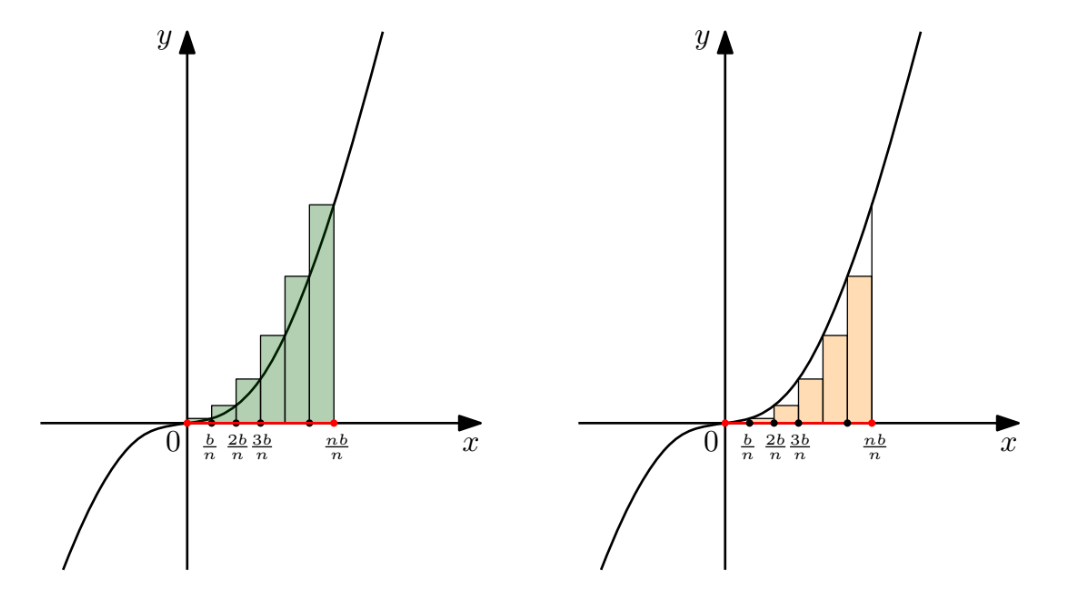
\includegraphics[width=0.7\textwidth]{img/lecture24/definite_integral}
		\end{center}
	\end{example}
	
	\begin{explanation}
	Площадь столбиков на левой картинке:
	\[ S_1 = \sum_{k = 1}^n \bigg(\frac{kb}{n}\bigg)^3 \frac{b}{n} = \sum_{k = 1}^n \frac{b^4}{n^4} \cdot k^3 = \frac{b^4}{n^4} \sum_{k = 1}^n k^3 = \frac{b^4}{n^4} (1 + 2 + ... + n)^2 (*) = \frac{b^4}{n^4} \frac{(n + 1)^2n^2}{4} \]
	
	(*) Формула суммы кубов доказывается по индукции.
	
	Площадь фигуры под графиком заведомо покрывается зелёными столбиками.
	
	Площадь столбиков на правой картинке:
	\[ S_2 = \sum_{k = 1}^n \bigg(\frac{(k - 1)b}{n}\bigg)^3 \frac{b}{n} = \sum_{k = 1}^n \frac{(k - 1)^3b^4}{n^4} \cdot k^3 = \frac{b^4}{n^4} \sum_{k = 1}^n (k - 1)^3 = \frac{b^4}{n^4} (1 + 2 + ... + n)^2 = \]
	\[ = \frac{b^4}{n^4} \frac{(n - 1)^2n^2}{4} \]
	
	Сумма $S_2$ меньше площади фигуры под графиком.
	\[ \lim_{n \to \infty} S_1 = \lim_{n \to \infty} \frac{b^4}{n^4} \frac{(n + 1)^2n^2}{4} = \lim_{n \to \infty} \frac{b^4}{4} \frac{(n + 1)^2}{n^2} = \lim_{n \to \infty} \frac{b^4}{4} \bigg(1 + \frac{1}{n}\bigg)^2 = \frac{b^4}{4} \]
	\[ \lim_{n \to \infty} S_2 = \lim_{n \to \infty} \frac{b^4}{n^4} \frac{(n - 1)^2n^2}{4} = \lim_{n \to \infty} \frac{b^4}{4} \frac{(n - 1)^2}{n^2} = \lim_{n \to \infty} \frac{b^4}{4} \bigg(1 - \frac{1}{n}\bigg)^2 = \frac{b^4}{4} \]
	
	По теореме о зажатой последовательности площадь фигуры равна $\frac{b^4}{4}$. Но можно было получить ответ, посчитав интеграл: $\displaystyle\int x^3 dx = \frac{x^4}{4} + C$.
	\end{explanation}
	
	\section{Интеграл Римана}
	
	\begin{definition}
		\begin{itemize}
			
			\item \underline{Разбиением} $T$ отрезка $[a, b]$ называется набор точек
			$a = x_0 < x_1 < ... < x_n = b$.
			
			\item Отрезки $[x_{k - 1}, x_k]$ называются \underline{отрезками разбиения}. Длину отрезка $[x_{k - 1}, x_k]$ обозначим через $\Delta x_k = x_k - x_{k - 1}, k \geqslant 1$.
			
			\item Величина $\Delta_T := \displaystyle \max_{1 \leqslant k \leqslant n} \Delta x_k$ называется \underline{диаметром разбиения}.
			
			\item \underline{Размеченным разбиением} $(T, \xi)$ отрезка $[a, b]$ называется пара, состоящая из разбиения $T$ отрезка $[a, b]$ и набора точек $\xi = (\xi_1, ..., \xi_n), \xi_k \in [x_{k - 1}, x_k]$.
			
			\item \underline{Интегральной суммой} функции $f$, соответствующей размеченному разбиению $(T, \xi)$, называется выражение
			\[ \sigma(f, T, \xi) := \sum^{n}_{k = 1} f(\xi_k) \Delta x_k. \]
		\end{itemize}
	\end{definition}
	
	\begin{definition}
		Функция $f$ называется интегрируемой по Риману на отрезке
		$[a, b]$, если существует такое число $I$, что $\forall \epsilon > 0$ $\exists \delta > 0: \forall$ размеченного разбиения $(T, \xi)$ с диаметром разбиения $\Delta_T < \delta$ выполнено $|\sigma(f, T, \xi) - I| < \epsilon$.
		
		Число $I$ называют интегралом функции $f$ на отрезке $[a, b]$ и
		обозначают $\displaystyle\int^{b}_{a} f(x) \; dx$.
	\end{definition}
	
	\begin{explanation}
		Геометрически мы уменьшаем длину отрезков и увеличиваем их число.
	\end{explanation}
	
	\begin{example}
		\begin{enumerate}
			\item $\displaystyle\int^{b}_{a} 1 \; dx = b - a$;
			\item Функция $I_{\Q}$ не интегрируема ни на каком отрезке.
		\end{enumerate}	
	\end{example}
	
	\begin{explanation}
		\begin{enumerate}
			\item $\sigma(f, T, \xi) = \sum^{n}_{k = 1} f(\xi_k) \Delta x_k = \sum^{n}_{k = 1} 1 \cdot \Delta x_k = \sum^{n}_{k = 1} \Delta x_k = b - a.$ (функция $f(\xi_k) = 1$ $\forall k$)
			
			\item Функция Дирихле $I_{\Q} : \R \rightarrow {0, 1}$ определяется следующим образом:
			\[\displaystyle I_{\Q} = \left\{{
				\begin{matrix}
					1, & x \in \Q \\
					0, & x \in \I
				\end{matrix}
			}\right.\]
			$\forall$ разбиения $T$ можно взять $\xi \in \Q$, $\zeta \in \I$ (внутри любого отрезка разбиения можно взять рациональное и иррациональное число)
			
			Тогда $\sigma(I_{\Q}, T, \xi) = \sum^{n}_{k = 1} I_{\Q}(\xi_k) \Delta x_k = \sum^{n}_{k = 1} 1 \cdot \Delta x_k = \sum^{n}_{k = 1} \Delta x_k = b - a$ и $\sigma(I_{\Q}, T, \zeta) = \sum^{n}_{k = 1} I_{\Q}(\zeta_k) \Delta x_k = \sum^{n}_{k = 1} 0 \cdot \Delta x_k = 0$.
			
			Тогда для любого $T$ с любым диаметром разбиения можно взять разметку, такую что иногда сумма равна $b - a$, иногда 1. Если $b - a \neq 0$, то функция не интегрируема.
		\end{enumerate}	
	\end{explanation}
    
    \section*{Лекция 25: Интеграл Римана, суммы Дарбу}
    
    \begin{sentence}
    	Если функция $f$ интегрируема по Риману на отрезке $[a, b]$, то она ограничена на этом отрезке.
    \end{sentence}
    
    \begin{proof}
    	Пусть $f$ - интегрируема на $[a, b]$. 
    	
    	Тогда $\exists I \in \R : \forall \epsilon > 0$ $\exists \delta > 0$  $\forall (T, \xi)$ с $\Delta_T < \delta \rightarrow |\sigma(f, T, \xi) - I| < \epsilon \Leftrightarrow$ $\Leftrightarrow I - \epsilon < \sigma(f, T, \xi) < I + \epsilon$.
    	
    	$\sigma(f, T, \xi) = \sum^{n}_{k = 1} f(\xi_k) \Delta x_k.$
    	
    	Пусть $f$ - неограничена на $[a, b] \Rightarrow$ неограничена на одном из отрезков $\Delta_k,$ пусть на $\Delta_{k_0}$. Фиксируем $\xi_k$ для всех $k$ кроме $k_0$. Тогда $\sigma(f, T, \xi) = \sum^{n}_{k = 1} f(\xi_k) \Delta x_k = C + f(\xi_{k_0}) \Delta x_{k_0} \Rightarrow I - C - \epsilon < f(\xi_{k_0}) \Delta x_{k_0} < I - C + \epsilon \Rightarrow \frac{I - C - \epsilon}{\Delta x_{k_0}} < f(\xi_{k_0}) < \frac{I - C + \epsilon}{\Delta x_{k_0}}$ - противоречие, функция ограничена.
    \end{proof}
    
    \begin{sentence}[Линейность интеграла]
    	Пусть $f$ и $g$ интегрируемы по Риману на отрезке $[a, b]$. Тогда
    	для произвольных чисел $\alpha$, $\beta$ функция $\alpha f + \beta g$ интегрируема по Риману на отрезке $[a, b]$ и
    	\[ \displaystyle\int^b_a \alpha f(x) + \beta g(x) \; dx = \alpha \displaystyle\int^b_a f(x) \; dx + \beta \displaystyle\int^b_a g(x) \; dx. \]
    \end{sentence}
    
    \begin{proof}
    	$f$ - интегрируема на $[a, b] \Rightarrow \forall \epsilon > 0$ $\exists \delta_1 > 0 : \forall (T, \xi)$ с $\Delta_T < \delta_1 \rightarrow |\sigma(f, T, \xi) - I_1| < \epsilon.$ 
    	
    	$g$ - интегрируема на $[a, b] \Rightarrow \forall \epsilon > 0$ $\exists \delta_2 > 0 : \forall (T, \xi)$ с $\Delta_T < \delta_2 \rightarrow |\sigma(g, T, \xi) - I_2| < \epsilon.$
    	
    	Размеченное разбиение $(T, \xi)$ взяли одно и то же для обоих интегралов.
    	
    	Первые два утверждения означают, что $I_1 = \int_a^b f(x) \; dx, I_2 = \int_a^b g(x) \; dx.$
    	
    	Рассмотрим интегральную сумму 
    	\[ \sigma(\alpha f + \beta g, T, \xi) = \sum_{k = 1}^n (\alpha f(\xi_k) + \beta g(\xi_k)) \Delta x_k = \sum_{k = 1}^n \alpha f(\xi_k) \Delta x_k + \sum_{k = 1}^n \beta g(\xi_k) \Delta x_k = \]
    	\[ = \alpha \sigma(f, T, \xi) + \beta \sigma(g, T, \xi) \]
    	
    	Фиксируем $\epsilon > 0$ и возьмём $\delta = \min{(\delta_1, \delta_2)} \Rightarrow |\sigma(\alpha f + \beta g, T, \xi) - \alpha I_1 - \beta I_2| = |\alpha \sigma(f, T, \xi) + \beta \sigma(g, T, \xi) - \alpha I_1 - \beta I_2| \leqslant |\alpha \sigma(f, T, \xi) - \alpha I_1| + |\beta \sigma(g, T, \xi) - \beta I_2| \leqslant |\alpha| \epsilon + |\beta| \epsilon = (|\alpha| + |\beta|) \epsilon$
    	
    	$\forall \epsilon = \frac{\epsilon'}{2(|\alpha| + |\beta|)} > 0$ $\exists \delta = \min{(\delta_1, \delta_2)} > 0 : \forall (T, \xi)$ с $\Delta_T < \delta \rightarrow |\sigma(\alpha f + \beta g, T, \xi) - \alpha I_1 - \beta I_2| \leqslant (|\alpha| + |\beta|) \frac{\epsilon'}{2(|\alpha| + |\beta|)} = \frac{\epsilon'}{2} < \epsilon'.$ 
    \end{proof}
    
    \begin{sentence}[Монотонность интеграла]
    	Пусть $f$ и $g$ интегрируемы по Риману на отрезке $[a, b]$. Если
    	$f(x) \leqslant g(x)$ $\forall x \in [a, b],$ то $\displaystyle\int^b_a f(x) \; dx \leqslant \displaystyle\int^b_a g(x) \; dx.$
    \end{sentence}
    
    \begin{proof}
    	$f(x) \leqslant g(x) \Leftrightarrow g(x) - f(x) \geqslant 0$ и $\int_a^b f(x) \; dx \leqslant \int_a^b g(x) \; dx \Leftrightarrow \int_a^b g(x) - f(x) \; dx \geqslant 0$ (пользуемся линейностью). Пусть $h(x) = g(x) - f(x) \Rightarrow$ требуется доказать, что $h(x) \geqslant 0 \Rightarrow \int_a^b h(x) \geqslant 0$.
    	
    	По определению $\forall \epsilon > 0$ $\exists \delta > 0 : \forall (T, \xi)$ c $\Delta_T < \delta \rightarrow  |\sigma(h, T, \xi) - \int_a^b h(x) \; dx| < \epsilon \Leftrightarrow \int_a^b h(x) - \epsilon < \underline{\sigma(h, T, \xi) < \int_a^b h(x) + \epsilon}$.
    	
    	$\sigma(h, T, \xi) \geqslant 0 (\text{т. к. } h(\xi_k) \geqslant 0 \Rightarrow \sum_{k = 1}^n h(\xi_k) \Delta x_k \geqslant 0) \Rightarrow \int_a^b h(x) + \epsilon > 0$ $\forall \epsilon > 0 \Rightarrow \int_a^b h(x) > -\epsilon$ $\forall \epsilon > 0 \Rightarrow \int_a^b h(x) \geqslant 0.$
    \end{proof}
    
    \begin{mention}
    	В частности, $\bigg|\displaystyle\int^b_a f(x) \; dx\bigg| \leqslant \displaystyle\int^b_a |f(x)| \; dx.$
    \end{mention}
    
    \begin{proof}
    	Далее мы докажем, что если $f(x)$ интегрируема, то и $|f(x)|$ интегрируема.
    	\[ -|f(x)| \leqslant f(x) \leqslant |f(x)|  \Rightarrow -\int_a^b |f(x)| \; dx \leqslant \int_a^b f(x) \; dx \leqslant \int_a^b |f(x)| \; dx \Rightarrow \]
    	\[ \Rightarrow \bigg| \int_a^b f(x) \; dx \bigg| \leqslant \int_a^b |f(x)| \; dx \]
    \end{proof}
    
    \chapter{Критерий Дарбу и классы интегрируемых функций}
    
    \section{Суммы и интегралы Дарбу}
    
    Фиксируем ограниченную функцию $f$, определённую на отрезке $[a, b]$.
    
    \begin{definition}
    	Для ограниченной на отрезке $[a, b]$ функции $f$ и разбиения $T$ определим \underline{нижнюю и верхнюю суммы Дарбу}:
    	\[s(f, T) := \sum^n_{k = 1}\inf_{x \in [x_{k - 1}, x_k]} f(x) \Delta x_k;\] (на каждом отрезке берём минимальное значение функции)
    	\[S(f, T) := \sum^n_{k = 1}\sup_{x \in [x_{k - 1}, x_k]} f(x) \Delta x_k.\] (на каждом отрезке берём максимальное значение функции)
    	
    	\underline{Нижним интегралом Дарбу} называется число $I_{*} = \displaystyle\sup_{T} s(f, T)$, а \underline{верхним ин-}
    	\underline{тегралом Дарбу} называется число $I^{*} = \displaystyle\inf_{T} S(f, T).$
    \end{definition}
    
    Сумма зелёных прямоугольников - это $s(f, T)$, сумма красных прямоугольников - это $S(f, T)$.
    
    \begin{center}
    	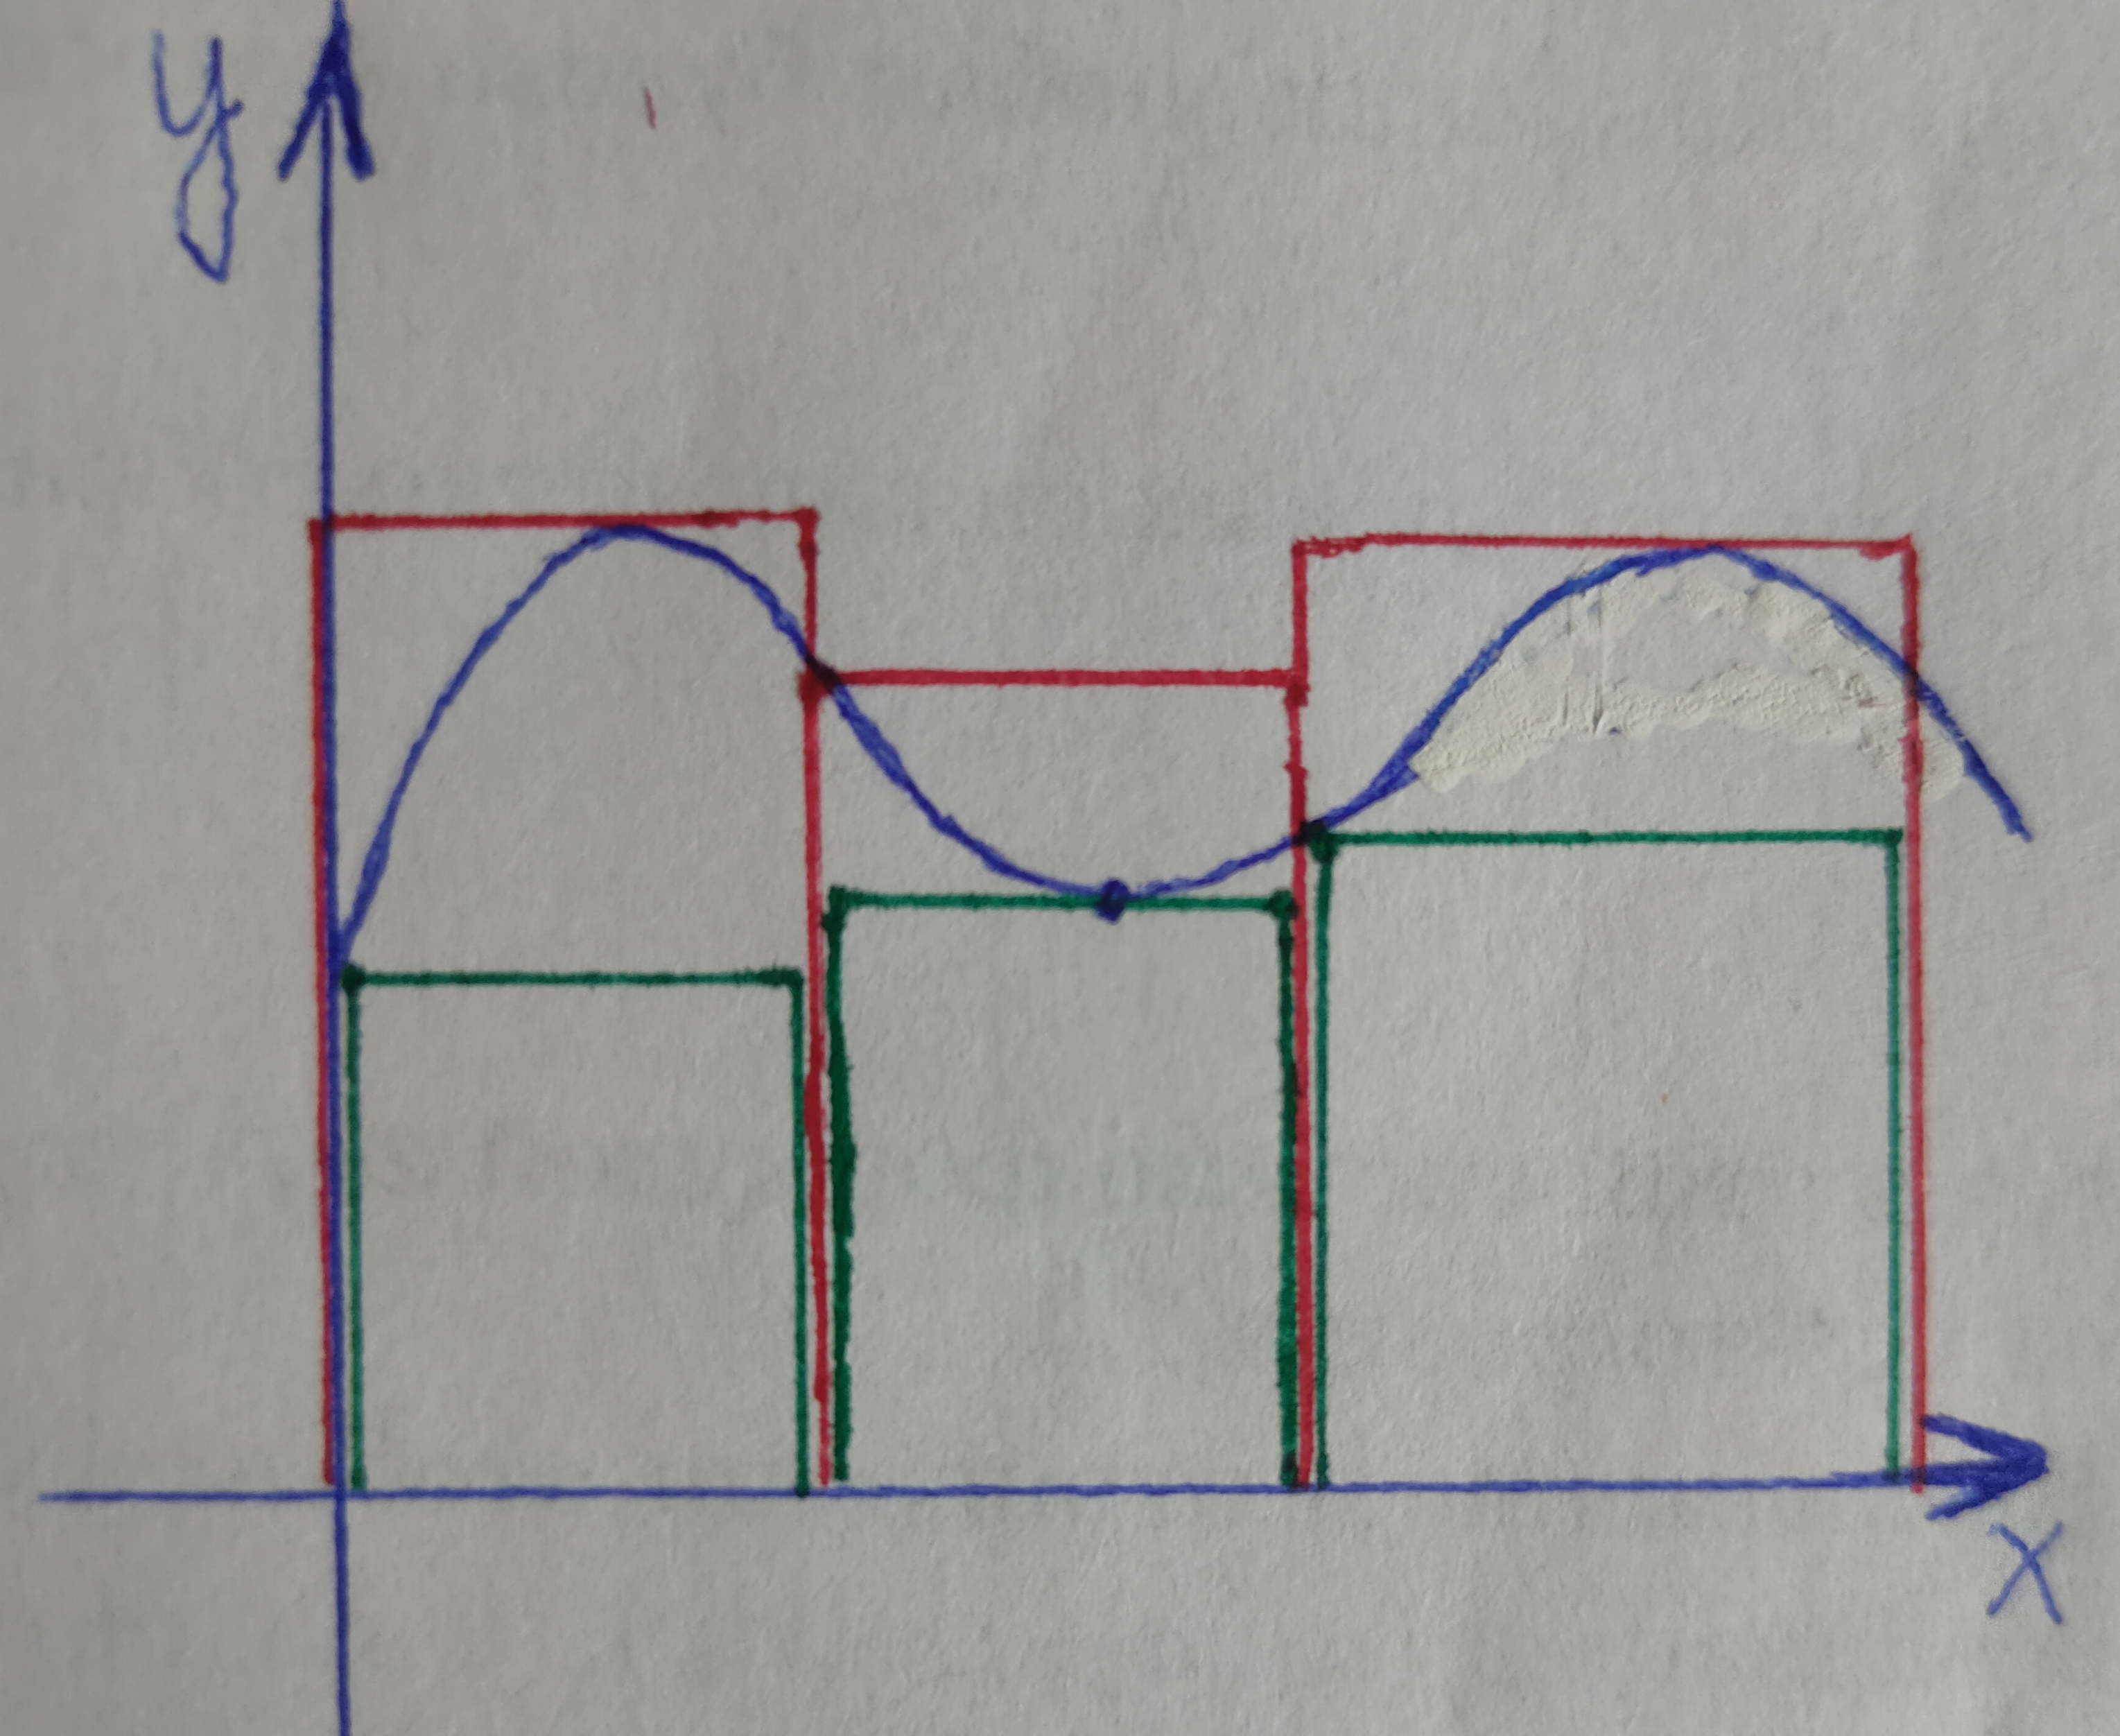
\includegraphics[width=0.4\textwidth]{img/lecture25/integral_darbu}
    \end{center}
    
    \section{Критерий Дарбу}
    
    \begin{lemma}
    	\begin{enumerate}
    		\item $s(f, T) \leqslant \displaystyle\inf_{\xi} \sigma(f, T, \xi) \leqslant \sigma(f, T, \xi) \leqslant \sup_{\xi}{\sigma(f, T, \xi)} \leqslant S(f, T);$
    		\item Если $T \subset T'$, то $s(f, T) \leqslant s(f, T')$ и $S(f, T') \leqslant S(f, T);$
    		\item $s(f, T_1) \leqslant s(f, T_1 \cup T_2) \leqslant S(f, T_1 \cup T_2) \leqslant S(f, T_2).$ 
    	\end{enumerate}
    \end{lemma}
    
    \begin{proof}
    	\begin{enumerate}
    		\item Докажем, что $\displaystyle s(f, T) = \inf_{\xi}{\sigma(f, T, \xi)}$
    		\begin{enumerate}
    			\item[$\leqslant$:] 
    			
    			$\forall \xi$ $\displaystyle s(f, T) = \sum_{k = 1}^n \inf_{\xi_k}{f(\xi_k) \Delta x_k} \leqslant \sum_{k = 1}^n f(\xi_k) \Delta x_k \Rightarrow s(f, T)$ - нижняя грань $\displaystyle \sum_{k = 1}^n f(\xi_k) \Delta x_k$.
    			
    			$\displaystyle \inf_{\xi}{\sum_{k = 1}^n f(\xi_k) \Delta x_k} = \inf_{\xi}{\sigma(f, T, \xi)}$ - точная нижняя грань $\Rightarrow \displaystyle s(f, T) \leqslant \inf_{\xi}{\sigma(f, T, \xi)}$.
    			
    			\item[$\geqslant$:] $\displaystyle s(f, T) = \sum_{k = 1}^n \inf_{\xi_k}{f(\xi_k) \Delta x_k}$
    			
    			По определенению инфимума $\forall \epsilon > 0$ $\displaystyle \exists \xi'_k \in \Delta_k : f(\xi'_k) \leqslant  \inf_{\xi_k}{f(\xi_k)} + \epsilon.$
    			
    			$\displaystyle \sigma(f, T, \xi') = \sum_{k = 1}^n f(\xi'_k) \Delta x_k \leqslant \sum_{k = 1}^n \bigg(\inf_{\xi_k}{f(\xi_k)} + \epsilon \bigg) \Delta x_k = s(f, T) + \epsilon(b - a)$
    			
    			$\displaystyle \inf_{\xi}{\sigma(f, T, \xi)} \leqslant \sigma(f, T, \xi') \leqslant s(f, T) + \epsilon(b - a)$
    			
    			При $\epsilon \to 0$, то $\displaystyle \inf_{\xi}{\sigma{(f, T, \xi)}} \leqslant s(f, T)$.
    		\end{enumerate}
    		Второе и третье неравенство в цепочке очевидное.
    		Четвёртое неравенство на самом деле является равенством и доказывается как первое равенство.
    		\item Рассмотрим отрезок $[a, b]$. На нём определено разбиение $T$. Теперь рассмотрим измельчение разбиения $T'$. Оно содержит те же точки, что и в $T$, но добавлет ещё свои точки.
    		
    		Красные точки - точки разбиения $T$, красные и зелёные точки - точки измельчения $T'$.
    		\begin{center}
    			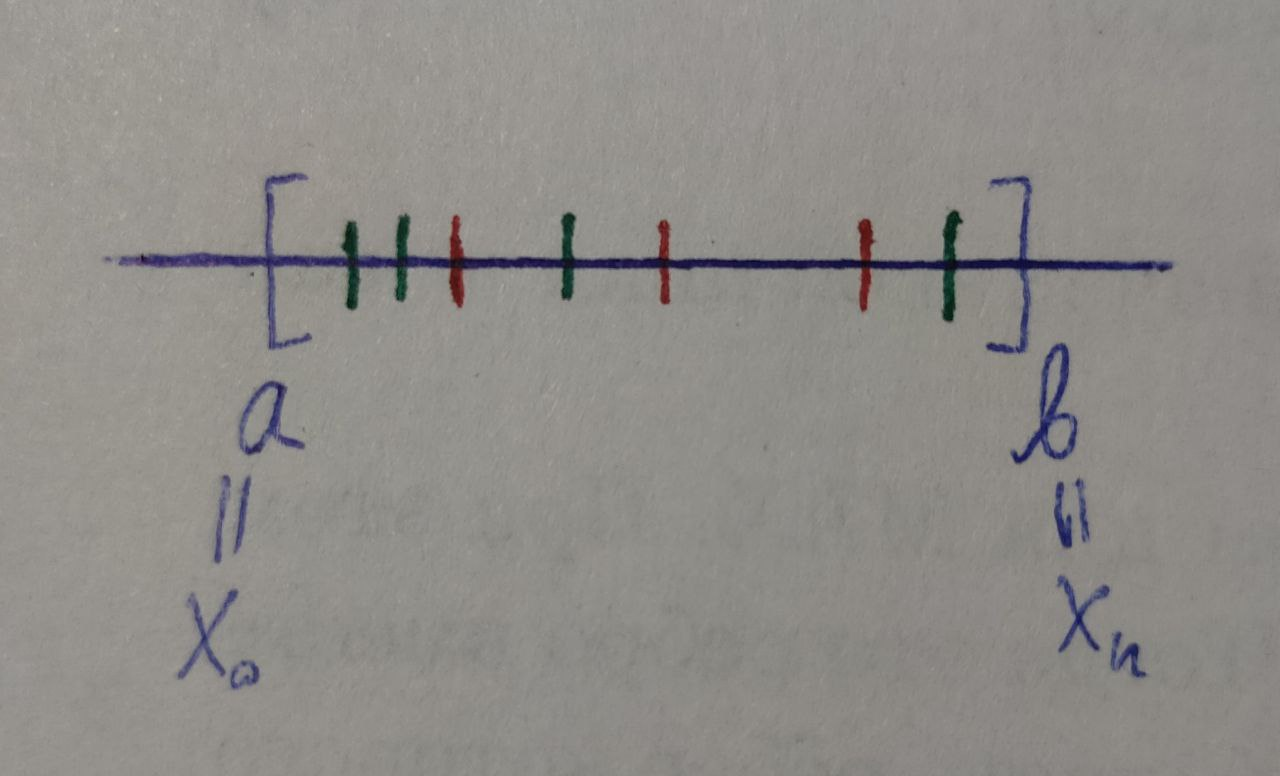
\includegraphics[width=0.3\textwidth]{img/lecture26/segment_division}
    		\end{center}
    		Пусть подотрезки $\Delta_k \in T$, а подотрезки $\Delta'_k \in T'$, $T \subset T'$. Рассмотрим отрезок $\Delta_k$ и будем считать, что он разбился на $k_j$ отрезков. Поэтому отрезок $\Delta'_k$ мы будем индексировать двумя индексами, первый номер - номер отрезка $\Delta_k$, в которым он лежит, второй номер - номер отрезка $\Delta'_k$ внутри отрезка $\Delta_k$.
    		\begin{center}
    			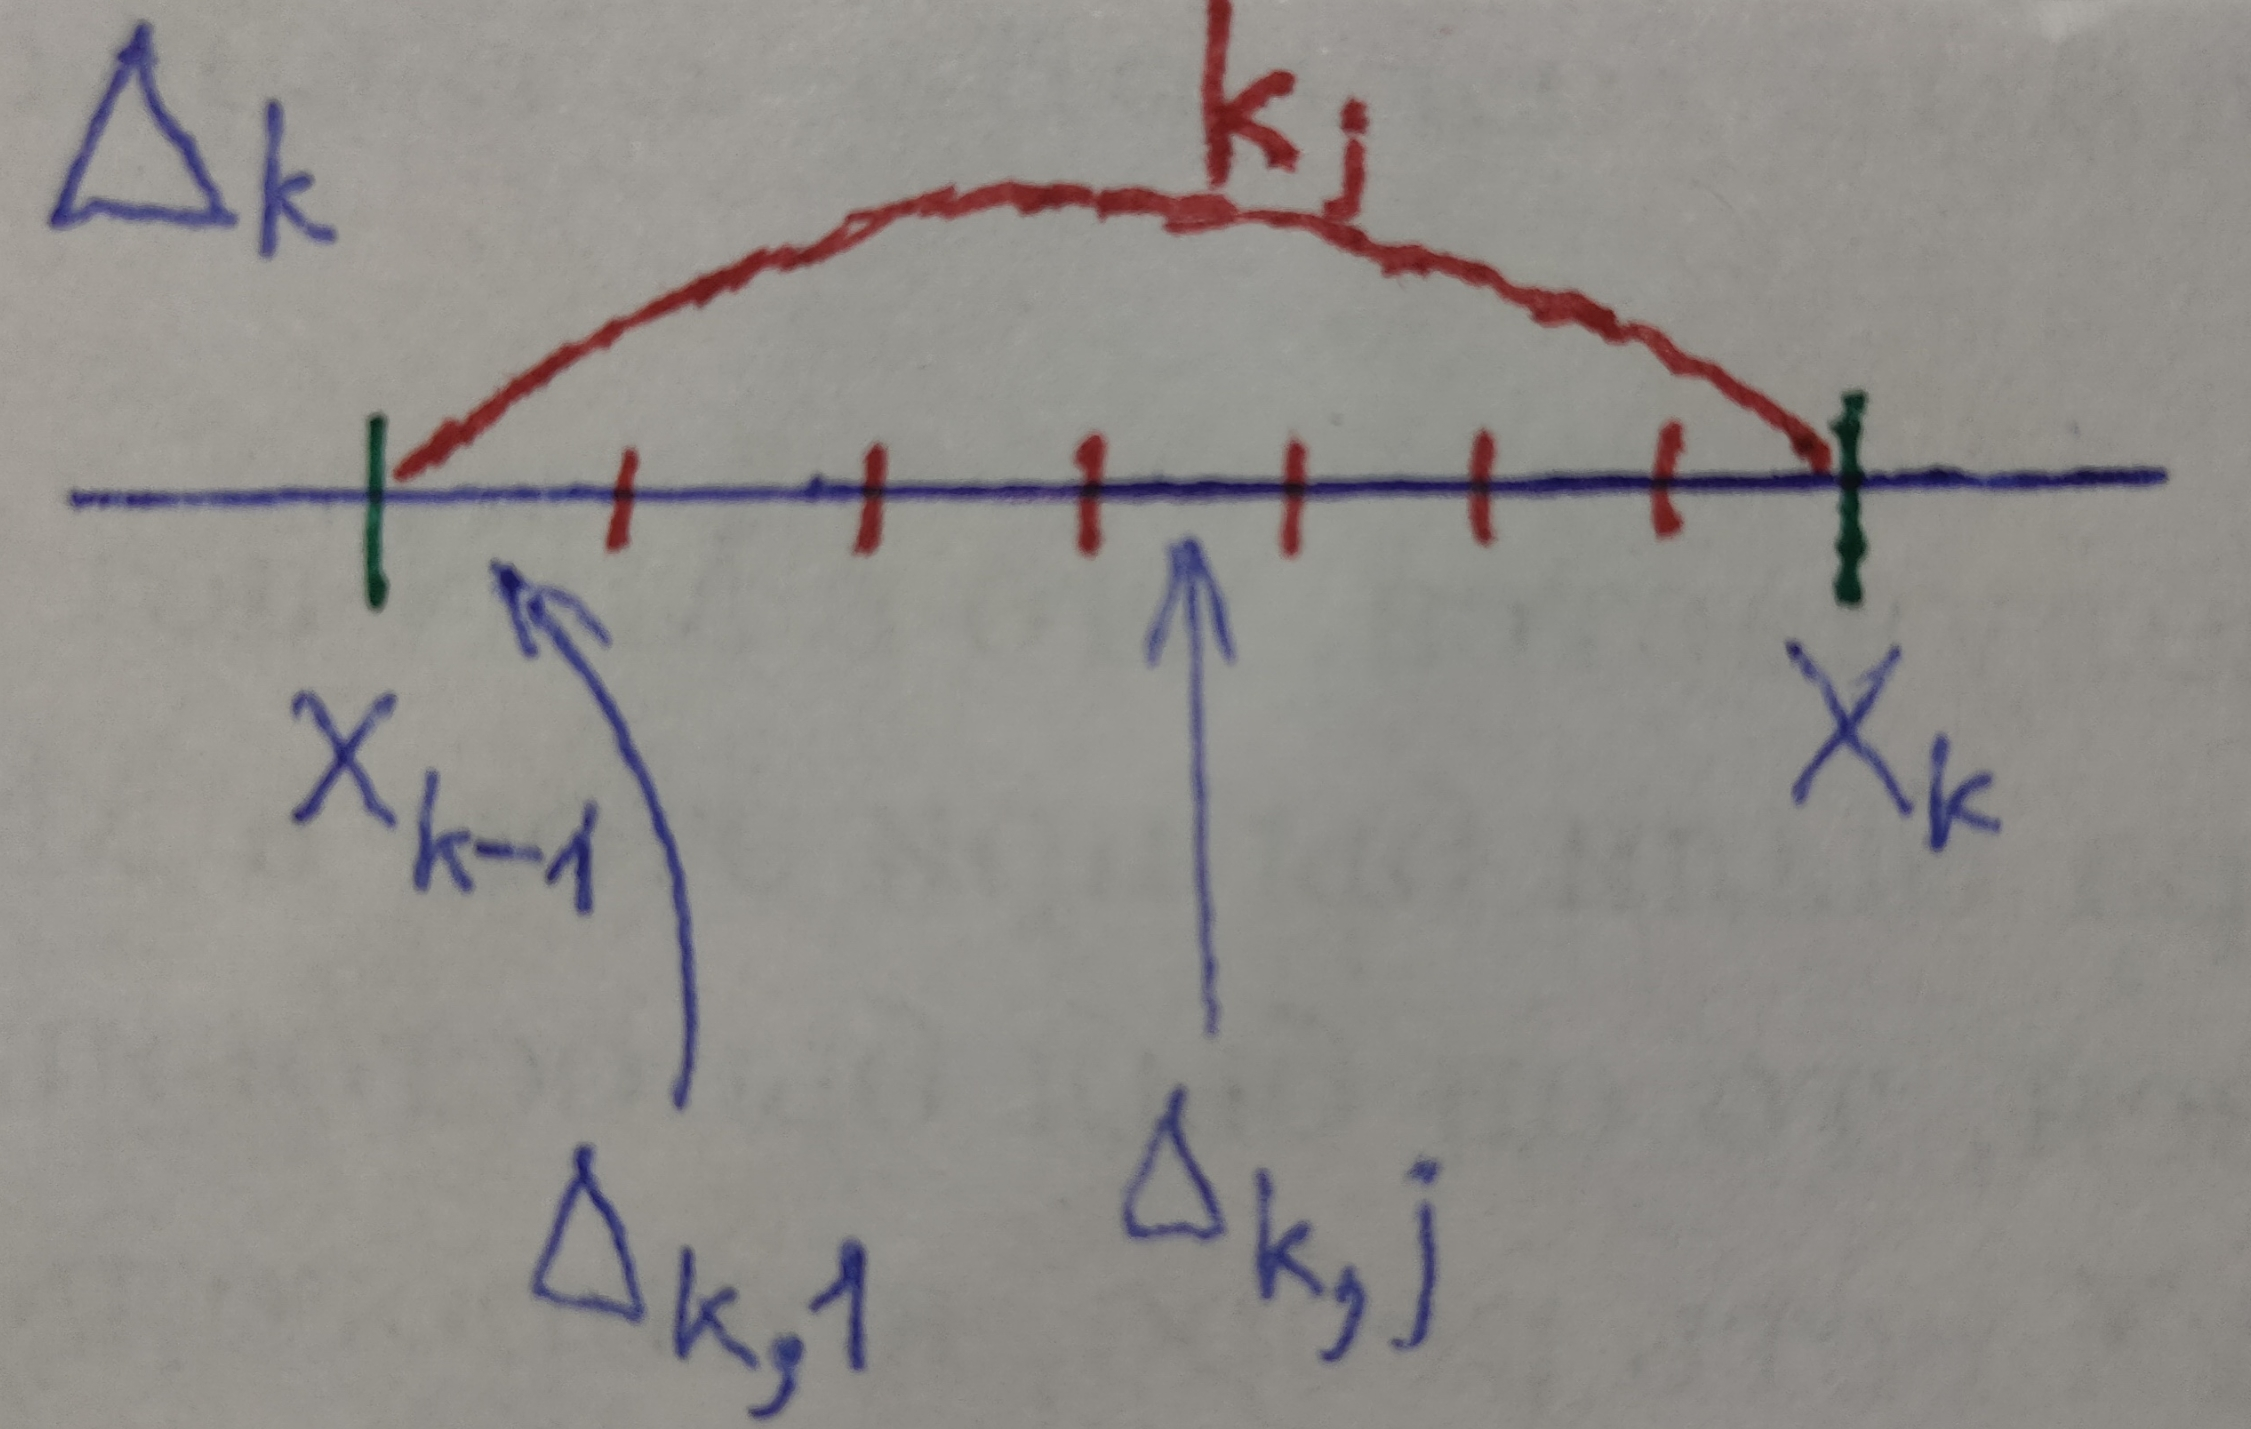
\includegraphics[width=0.3\textwidth]{img/lecture26/notations}
    		\end{center}
    		Тогда
    		\[ s(f, T') = \sum_{k = 1}^n\sum_{j = 1}^{k_j} \inf_{\xi \in \Delta_{k, j}}{f(\xi) \cdot \Delta x_{k, j}} \]
    		Приэтом на нескольких маленьких отрезках инфимум не меньше инфимума на одном большом отрезке, потому что на большом отрезке у нас есть больше точек, из которых мы можем выбрать меньшее значение. Если инфимум достигался на красном отрезке, то этот отрезок принадлежит большому, поэтому мы можем взять точку принадлежащую красному отрезку и получить инфимум на большом отрезке не больше, чем на маленьких. Поэтому
    		\[ s(f, T') = \sum_{k = 1}^n\sum_{j = 1}^{k_j} \inf_{\xi \in \Delta_{k, j}}{f(\xi) \cdot \Delta x_{k, j}} \geqslant \sum_{k = 1}^n\sum_{j = 1}^{k_j} \inf_{\xi \in \Delta_k}{f(\xi) \cdot \Delta x_{k, j}} \]
    		Продолжаем преобразования.
    		\[ \sum_{k = 1}^n \sum_{j = 1}^{k_j} \inf_{\xi \in \Delta_k}{f(\xi) \cdot \Delta x_{k, j}} = \sum_{k = 1}^n \inf_{\xi \in \Delta_k}{f(\xi) \sum_{j = 1}^{k_j} \Delta x_{k, j}} = \sum_{k = 1}^n \inf_{\xi \in \Delta_k}{f(\xi) \Delta x_k} = S(f, T) \]
    		Второе неравенство доказывается аналогично.
    		\item
    		\[ T_1 \subset T_1 \cup T_2 \Rightarrow \text{(из пункта 2) } s(f, T) \leqslant s(f, T_1 \cup T_2) \]
    		\[ \text{(из пункта 1) } s(f, T_1 \cup T_2) \leqslant S(f, T_1 \cup T_2) \]
    		\[ T_1 \cup T_2 \supset T_2 \Rightarrow \text{(из пункта 2) } S(f, T_1 \cup T_2) \leqslant S(f, T_2) \]
    	\end{enumerate}
    \end{proof}
    
    \section*{Лекция 26: Интеграл Римана, суммы Дарбу}
    
    \begin{lemma}
    	$\forall \epsilon > 0$ $\exists \delta > 0:$ $\forall T$ с $\Delta_T < \delta$ выполнено $I_{*} \leqslant s(f, T) + \epsilon$ и $I^{*} \geqslant S(f, T) - \epsilon$.
    \end{lemma}
    
    \begin{proof}
    	По определению супремума
    	\[ I_{*} = \sup_T{s(f, T)} \Rightarrow \forall \epsilon > 0 \text{ } \exists T_{\epsilon} : I_{*} \leqslant s(f, T_{\epsilon}) + \epsilon \]
    	Рассмотрим произвольное разбиение $T$
    	\[ s(f, T_{\epsilon} \cup T) \geqslant \text{(пункт 2 предыдущей леммы)} s(f, T_{\epsilon}) \geqslant I_{*} - \epsilon \]
    	
    	Точки из разбиения $T$ окрасим в красный цвет, точки из $T_{\epsilon}$ - в чёрный цвет.
    	
    	\begin{center}
    		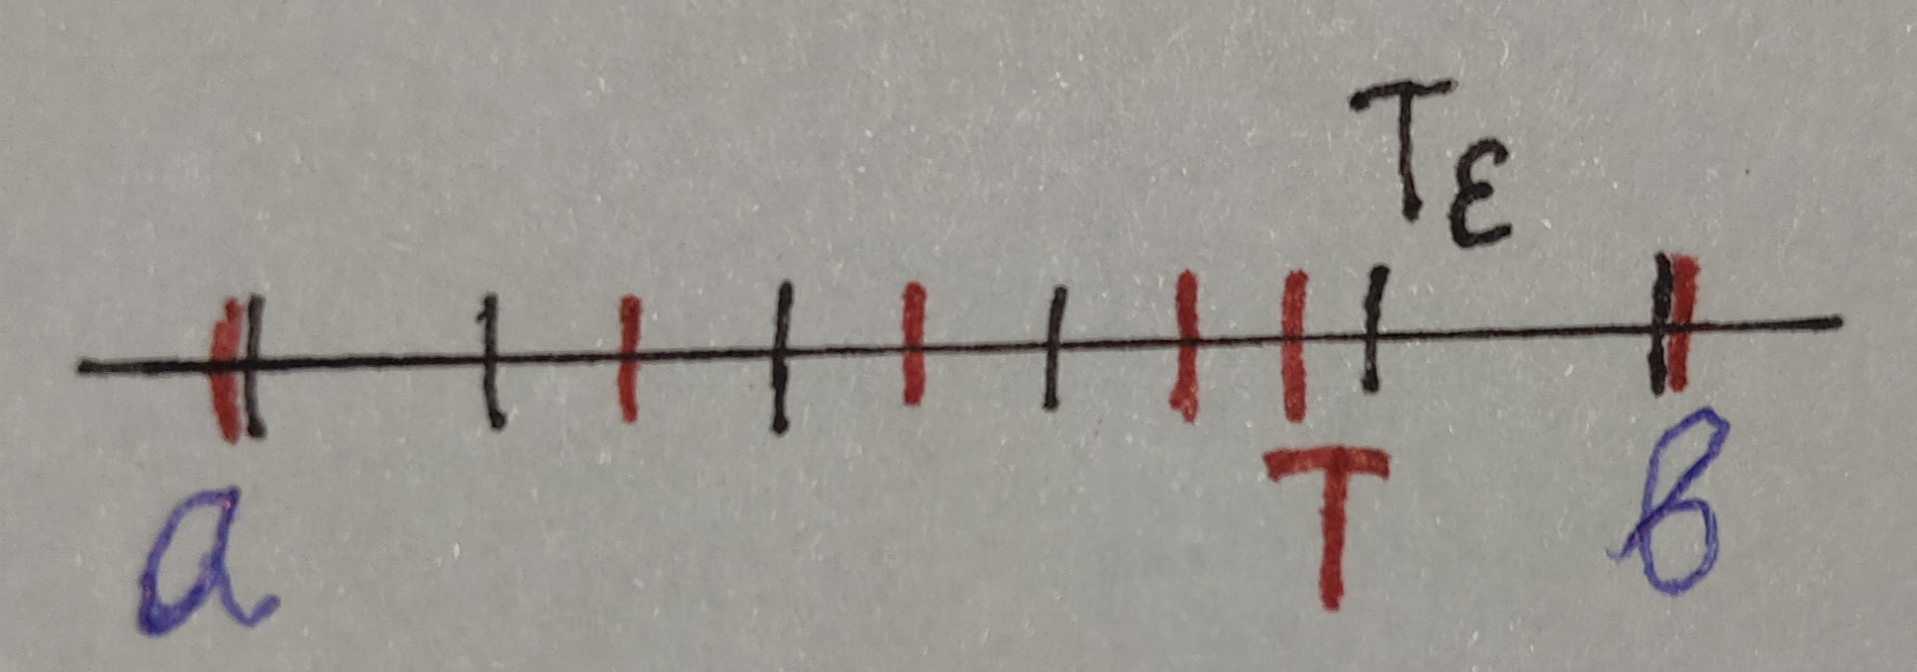
\includegraphics[width=0.2\textwidth]{img/lecture26/coloring_segments}
    	\end{center}
    	
    	Точки $T_{\epsilon}$ делят отрезок c красными концами на число чёрных точек + 1. Тогда точки из $T_{\epsilon}$ могут разбить на не более, чем $2|T_{\epsilon}|$ отрезков, потому что максимум достигается, когда в каждом отрезке мы ставим по одной чёрной точке (т. е. разбиваем отрезок на два).
    	
    	\begin{center}
    		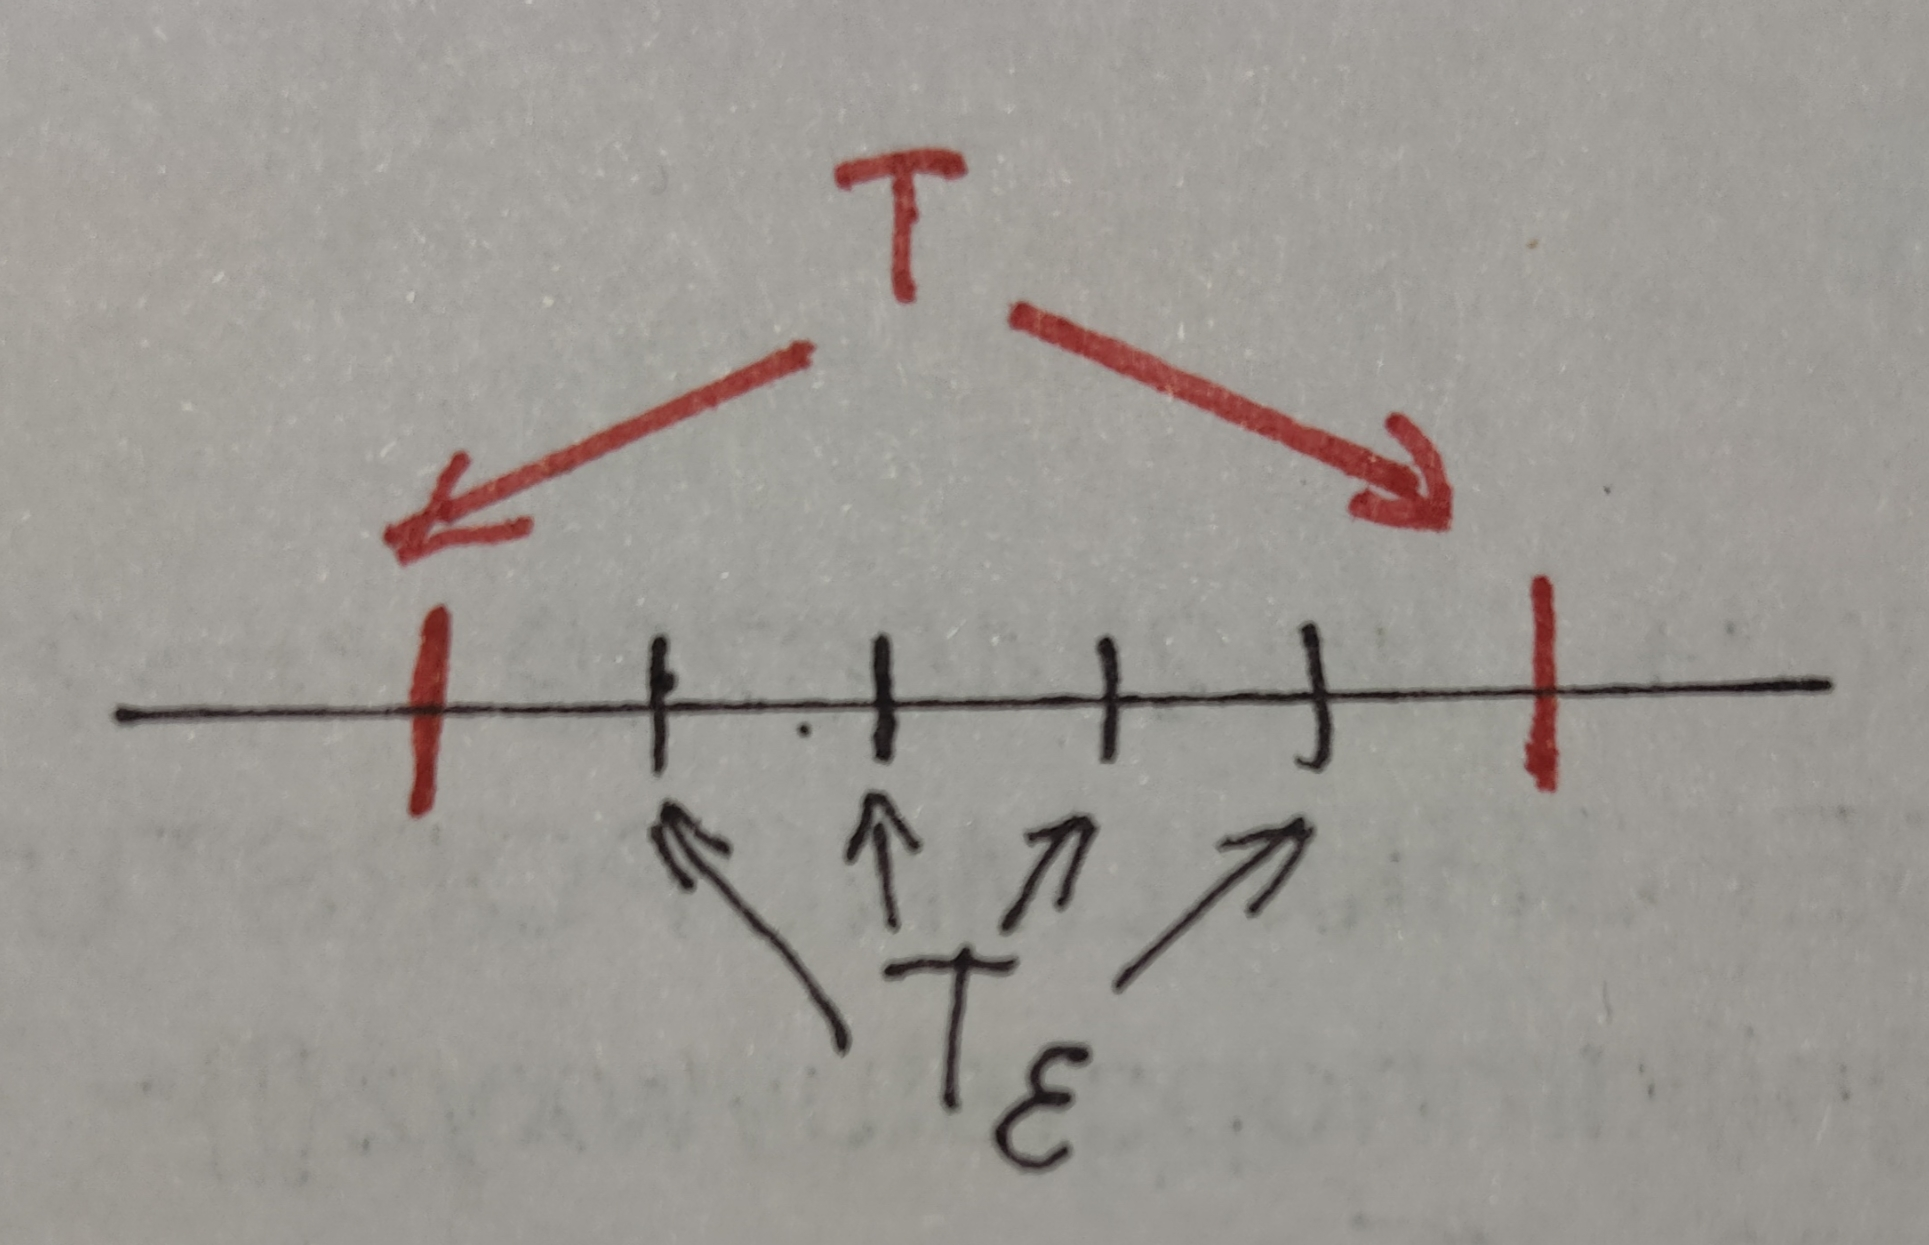
\includegraphics[width=0.2\textwidth]{img/lecture26/segment_number_estimation}
    	\end{center}
    	
    	\underline{Пояснение.} Здесь $\Delta_k$ - отрезок $[x_k, x_{k + 1}]$, подразумеваем под знаком суммы сумму по всем отрезкам, которые образуются этим множеством точек (отрезок образуют соседние точки, т. е. внутри отрезка других точек разбиения нет).
    	\[ s(f, T_{\epsilon} \cup T) = \sum_{\Delta_k \in T_{\epsilon} \cup T} \inf_{\xi \in \Delta_k} {f(\xi) \cdot \Delta x_k} = \sum_{\Delta_k \in T_{\epsilon} \cup T \text{ и } \Delta_k \in T} \inf_{\xi \in \Delta_k} {f(\xi) \cdot \Delta x_k} + \]
    	\[ + \sum_{\Delta_k \in T_{\epsilon} \cup T \text{ и } \Delta_k \not\in T} \inf_{\xi \in \Delta_k} {f(\xi) \cdot \Delta x_k} = (*) \]
    	Первая сумма - сумма отрезков с красными концами, вторая сумма - сумма остальных отрезков (т. е. либо оба конца чёрные, либо один конец чёрный, а другой - красный).
    	Первое слагаемое выразим как разность суммы по всем отрезкам с красными концами и суммы по всем отрезкам с красными концами, но с чёрными точками внутри.
    	\[ (*) = \sum_{\Delta_k \in T} \inf_{\xi \in \Delta_k} {f(\xi) \Delta x_k} - \sum_{\Delta_k \in T \text{ и } \Delta_k \not\in T \cup T_{\epsilon}} {\inf_{\xi \in \Delta_k} {f(\xi) \cdot \Delta x_k}} + \sum_{\Delta_k \in T_{\epsilon} \cup T \text{ и } \Delta_k \not\in T} {\inf_{\xi \in \Delta_k} {f(\xi) \cdot \Delta x_k}} \leqslant \]
    	\[ \leqslant s(f, T) + 2\sup_{x \in [a, b]} {|f(x)| \cdot \Delta_T \cdot 2|T_{\epsilon}|} \]
    	В конце - грубая оценка для последних двух слагаемых.
    	
    	Возьмём $\displaystyle \delta = \frac{\epsilon}{\displaystyle2\sup_{x \in [a, b]} {|f(x)| \cdot 2|T_{\epsilon}|}}$. Тогда для $T$ c $\Delta_T < \delta$
    	\[ I_{*} \leqslant s(f, T_{\epsilon}) + \epsilon \leqslant s(f, T \cup T_{\epsilon}) + \epsilon \leqslant s(f, T) + 2\sup_{x \in [a, b]} {|f(x)| \cdot \Delta_T \cdot 2|T_{\epsilon}|} + \epsilon < \]
    	\[ < s(f, T) + 2\sup_{x \in [a, b]} {|f(x)| \cdot \delta \cdot 2|T_{\epsilon}|} + \epsilon = s(f, T) + \epsilon + \epsilon = s(f, T) + 2\epsilon \]
    	
    	Заменой $\epsilon = \frac{\epsilon'}{2}$ получаем $I_{*} \leqslant s(f, T) + \epsilon'$.
    	
    	Аналогично доказывается, что $I^{*} \geqslant S(f, T) - \epsilon$.
    	
    	\underline{Уточнение.} Если фиксируем $\epsilon$, то $T_{\epsilon}$ - фиксированное число. $f(x)$ интегрируема $\Rightarrow$ она ограничена (по предложению 9.5) $\Rightarrow$ супремум ограничен, поэтому такое $\delta$ рассматривать корректно.
    \end{proof}
    
    \begin{theorem}[Критерий Дарбу]
    	Ограниченная функция $f$ интегрируема по Риману на отрезке $[a, b]$ тогда и только тогда, когда $I^{*} = I_{*}$.
    \end{theorem}
    
    \begin{proof}
    	\begin{enumerate}
    		\item[$\Rightarrow$] Если функция интегрируема, то 
    		\[ \forall \epsilon > 0 \text{ } \exists \delta > 0: \forall (T, \xi) \text{ с } \Delta_T < \delta \rightarrow |\sigma(f, T, \xi) - I| < \epsilon \]
    		\[ I - \epsilon < \sigma(f, T, \xi) < I + \epsilon \]
    		\[ I - \epsilon \leqslant \inf_{\xi} {\sigma(f, T, \xi)} = s(f, T) \leqslant \sup_{T} {s(f, T)} = I_{*} \]
    		\[ I^{*} = \inf_{T} {S(f, T)} \leqslant S(f, T) = \sup_{\xi} {\sigma(f, T, \xi)} \leqslant I + \epsilon \]
    		
    		Докажем, что $I_{*} \leqslant I^{*}$:
    		\[ \forall T_1, T_2 \text{ } s(f, T_1) \leqslant S(f, T_2) \Rightarrow \sup_{T_1} {s(f, T_1)} \leqslant S(f, T_2) \Rightarrow \sup_{T_1} {s(f, T_1)} \leqslant \inf_{T_2} {S(f, T_2)} \]
    		Тогда
    		\[ I - \epsilon \leqslant I_{*} \leqslant I^{*} \leqslant I + \epsilon \]
    		Устремляя $\epsilon \to 0$, получаем, что $I_{*} = I^{*}$.
    		\item[$\Leftarrow$] $I = I_{*} = I^{*}$
    		\[ \forall \epsilon > 0 \text{ } \exists \delta > 0 : \forall T \text{ с } \Delta_T < \delta \rightarrow I - \epsilon = I_{*} - \epsilon \leqslant (\text{лемма 10.3}) \text{ } s(f, T) \leqslant \]
    		\[ \leqslant \sigma(f, T, \xi) \leqslant S(f, T) \leqslant (\text{лемма 10.3}) \text{ } I^{*} + \epsilon = I + \epsilon \Rightarrow |\sigma(f, T, \xi) - I| < \epsilon, \]
    		что есть определение интеграла.
    	\end{enumerate}
    \end{proof}
    
    \section{Колебание функции}
    
    \begin{definition}
    	\underline{Колебанием} функции $f$ на отрезке $\Delta$ называется число
    	\[ \omega(f, \Delta) := \sup_{x, y \in \Delta}{|f(x) - f(y)|} = \sup_{x \in \Delta}{f(x)} - \inf_{y \in \Delta}{f(y)}. \]
    \end{definition}
    
    \begin{explanation}
    	\begin{enumerate}
    		\item В одну сторону
    		\[ \forall x, y \in \Delta \text{ } f(x) - f(y) \leqslant \sup_{x, y \in \Delta} {(f(x))} - f(y) \leqslant \sup_{x \in \Delta} {f(x)} - \inf_{y \in \Delta} {f(y)} \Rightarrow \]
    		\[ \Rightarrow \sup_{x, y \in \Delta}{|f(x) - f(y)|} \leqslant \sup_{x \in \Delta}{f(x)} - \inf_{y \in \Delta}{f(y)} \] 
    		\item В другому сторону
    		
    		По определению супремума и инфимума
    		\[ \forall \delta > 0 \text{ } \exists x_{\delta}: \sup_{x \in \Delta} {f(x)} \leqslant f(x_{\delta}) + \delta \]
    		\[ \forall \delta > 0 \text{ } \exists y_{\delta}: \inf_{y \in \Delta} {f(y)} \geqslant f(y_{\delta}) - \delta \]
    		Тогда
    		\[ \sup_{x \in \Delta} {f(x)} - \inf_{y \in \Delta}{f(y)} \leqslant f(x_{\delta}) - f(y_{\delta}) + 2\delta \leqslant  \sup_{x, y \in \Delta} {|f(x) - f(y)|} + 2\delta \Rightarrow \]
    		\[ \Rightarrow \sup_{x \in \Delta} {f(x)} - \inf_{y \in \Delta}{f(y)} \leqslant  \sup_{x, y \in \Delta} {|f(x) - f(y)|} \text{ при } \delta \to 0 \]
    	\end{enumerate}
    \end{explanation}
    
    \section*{Лекция 27: Интегрируемость по Риману различных классов функций}
    
    \begin{theorem}
    	Пусть $f$ - ограниченная на отрезке $[a, b]$ функция. Тогда следующие условия эквивалентны:
    	\begin{enumerate}
    		\item $I^{*} = I_{*}$;
    		\item Функция $f$ интегрируема на $[a, b]$;
    		\item $\forall \epsilon > 0$ $\exists \delta > 0: \forall T$ с $\Delta_T < \delta:$
    		\[ \sum_{k = 1}^{n} \omega(f, \Delta_k) \Delta x_k < \epsilon; \]
    		\item $\forall \epsilon > 0$ $\exists T:$
    		\[ \sum_{k = 1}^{n} \omega(f, \Delta_k) \Delta x_k < \epsilon; \]
    	\end{enumerate}
    \end{theorem}
    
    \begin{proof}
    	Заметим, что
    	\[ S(f, T) - s(f, T) = \sum_{k = 1}^n \sup_{\xi \in \Delta_k} f(\xi) \Delta x_k - \sum_{k = 1}^n \inf_{\xi \in \Delta_k} f(\xi) \Delta x_k = \]
    	\[ = \sum_{k = 1}^n \bigg(\sup_{\xi \in \Delta_k} f(\xi) \Delta x_k - \inf_{\xi \in \Delta_k} f(\xi) \Delta x_k\bigg) = \sum_{k = 1}^n \omega(f, \Delta_k) \Delta x_k \]
    	
    	\begin{enumerate}
    		\item[$1 \Rightarrow 2$] Применяем критерий Дарбу.
    		\item[$2 \Rightarrow 3$] Пусть $f$ - интегрируемая функция на $[a, b]$. Тогда $I^{*} = I_{*} = I$.
    		
    		По лемме 10.3
    		\[ \forall \epsilon > 0 \text{ } \exists \delta > 0: \forall T \text{ c } \Delta_T < \delta:
    		\displaystyle \left\{{
    			\begin{matrix}
    				I = I^{*} \geqslant S(f, T) - \epsilon, \\
    				I = I_{*} \leqslant s(f, T) + \epsilon. \\
    			\end{matrix}
    		}\right. \Rightarrow \]
    		\[ \Rightarrow I - I \leqslant s(f, T) - S(f, T) + 2\epsilon \]
    		По замечанию заключаем
    		\[ \sum_{k = 1}^n \omega(f, \Delta_k) \Delta x_k \leqslant 2\epsilon \]
    		\item[$3 \Rightarrow 4$] По предыдущему пункту существует такое $T$ с диаметром $\Delta_T < \delta$, значит и просто $T$ существует.
    		\item[$4 \Rightarrow 1$] В доказательстве критерия Дарбу мы получили следующую цепочку неравенств
    	    \[ s(f, T) \leqslant I_{*} \leqslant I^{*} \leqslant S(f, T) \]
    	    Тогда
    	    \[ 0 \leqslant I^{*} - I_{*} \leqslant S(f, T) - s(f, T) \leqslant \sum_{k = 1}^n \omega(f, \Delta_k) \Delta x_k < \epsilon \Rightarrow \text{ при } \epsilon \to 0 \text{ } I^{*} = I_{*} \]
    	\end{enumerate}
    \end{proof}
    
     \section{Интегрируемость модуля, квадрата и произведения функций}
    
    \begin{corollary}
    	Если $f$ интегрируема по Риману на отрезке $[a, b]$, то $|f|$ и $f^2$ интегрируемы по Риману на отрезке $[a, b]$ и для любого $[c, d] \subset [a, b]$ функция $f$ интегрируема по Риману на отрезке
    	$[c, d]$.
    \end{corollary}
    
    \begin{proof}
    	$f$ - интегрируема на $[a, b] \Leftrightarrow$ по пункту 4 теоремы 10.6 
    	\[ \forall \epsilon > 0 \text{ } \exists T: \sum_{k = 1}^n \omega(f, \Delta_k) \Delta x_k < \epsilon. \]
    	\underline{Доказательство для модуля функции}
    	
    	(Неравенство треугольника: $|A| - |B| \leqslant |A - B|, |B| - |A| \leqslant |A - B| \Rightarrow ||A| - |B|| \leqslant |A - B|$)
    	\[ \omega(|f|, \Delta_k) = \sup_{x, y \in \Delta_k} {||f(x)| - |f(y)||} \leqslant \sup_{x, y \in \Delta_k} {|f(x) - f(y)|} = \omega(f, \Delta_k) \Rightarrow \]
    	\[ \Rightarrow 0 \leqslant \sum_{k = 1}^n {\omega(|f|, \Delta_k)} \Delta x_k \leqslant \sum_{k = 1}^n \omega(f, \Delta_k) \Delta x_k < \epsilon \]
    	\underline{Доказательство для квадрата функции}
    	\[ \omega(f^2, \Delta_k) = \sup_{x, y \in \Delta_k} {|f^2(x) - f^2(y)|} = \sup_{x, y \in \Delta_k} {|(f(x) - f(y))(f(x) + f(y))|} \leqslant \]
    	\[ \leqslant \sup_{x, y \in \Delta_k} {|f(x) - f(y)|(|f(x)| + |f(y)|)} \leqslant 2\sup_{x \in \Delta_k} {|f(x)|} \sup_{x, y \in \Delta_k} {|f(x) - f(y)|} = \]
    	\[ = 2\sup_{x \in \Delta_k} {|f(x)|} \cdot \omega(f, \Delta_k) \]
    	\[ \sum_{k = 1}^n \omega(f^2, \Delta_k) \Delta x_k \leqslant \sum_{k = 1}^n 2\sup_{x \in \Delta_k} {|f(x)| \omega(f, \Delta_k) \Delta x_k} \leqslant 2\sup_{x \in [a, b]} |f(x)| \sum_{k = 1}^n \omega(f, \Delta_k) \Delta x_k \leqslant \]
    	\[ \leqslant M \cdot \epsilon, \text{где M - константа}. \]
    	
    	В обоих случаях в конце мы применяем теорему 10.6 и заключаем, что функции интегрируемы на $[a, b]$.
    	
    	Интегрируемость функции на подотрезке докажем далее.
    \end{proof}
    
    \begin{corollary}
    	Если $f$ и $g$ интегрируемы на $[a, b]$, то и $f \cdot g$ интегрируема на $[a, b]$.
    \end{corollary}
    
    \begin{proof}
    	Если $f$ и $g$ интегрируемы, то $f - g$ и $f + g$ интегрируемы. Тогда их квадраты $(f - g)^2$ и $(f + g)^2$ интегрируемы. Следовательно, $\frac{1}{4}((f + g)^2 - (f - g)^2) = \frac{1}{4} \cdot 4fg = fg$ интегрируема.
    \end{proof}
    
    \section{Интегрируемость монотонной функции}
    
    \begin{corollary}
    	Если $f$ монотонна на $[a, b]$, то $f$ интегрируема по Риману на $[a, b]$.
    \end{corollary}
    
    \begin{proof}
    	Без ограничения общности пусть $f$ - возрастающая функция.
    	\[ \omega(f, \Delta_k) = f(x_k) - f(x_{k - 1}) \]
    	\[ \sum_{k = 1}^n \omega(f, \Delta_k) \cdot \Delta x_k = \sum_{k = 1}^n (f(x_k) - f(x_{k - 1})) \Delta x_k = (*) \]
    	Пусть $\Delta x_k = \Delta x_j$ $\forall k, j$. Тогда
    	\[ (*) = \Delta x_1 \sum_{k = 1}^n (f(x_k) - f(x_{k - 1})) = \Delta_T (f(b) - f(a)) \]
    	Следовательно, $\forall T -$ разбиение $[a, b]$ на одинаковые части с $\Delta_T < \frac{\epsilon}{f(b) - f(a)}$
    	\[ \sum_{k = 1}^n \omega(f, \Delta_k) \Delta x_k \leqslant \epsilon. \]
    	
        Для убывающей $f$ доказывается аналогично.
    \end{proof}
    
    \section{Равномерная непрерывность}
    
    \begin{definition}
    	\item Функция $f$ называется \underline{равномерно непрерывной} на
    	множестве $X$, если $\forall \epsilon > 0$ $\exists \delta > 0$ для которого из неравенства
    	$|x - y| < \delta$ следует $|f(x) - f(y)| < \epsilon.$
    \end{definition}
    
    \begin{center}
    	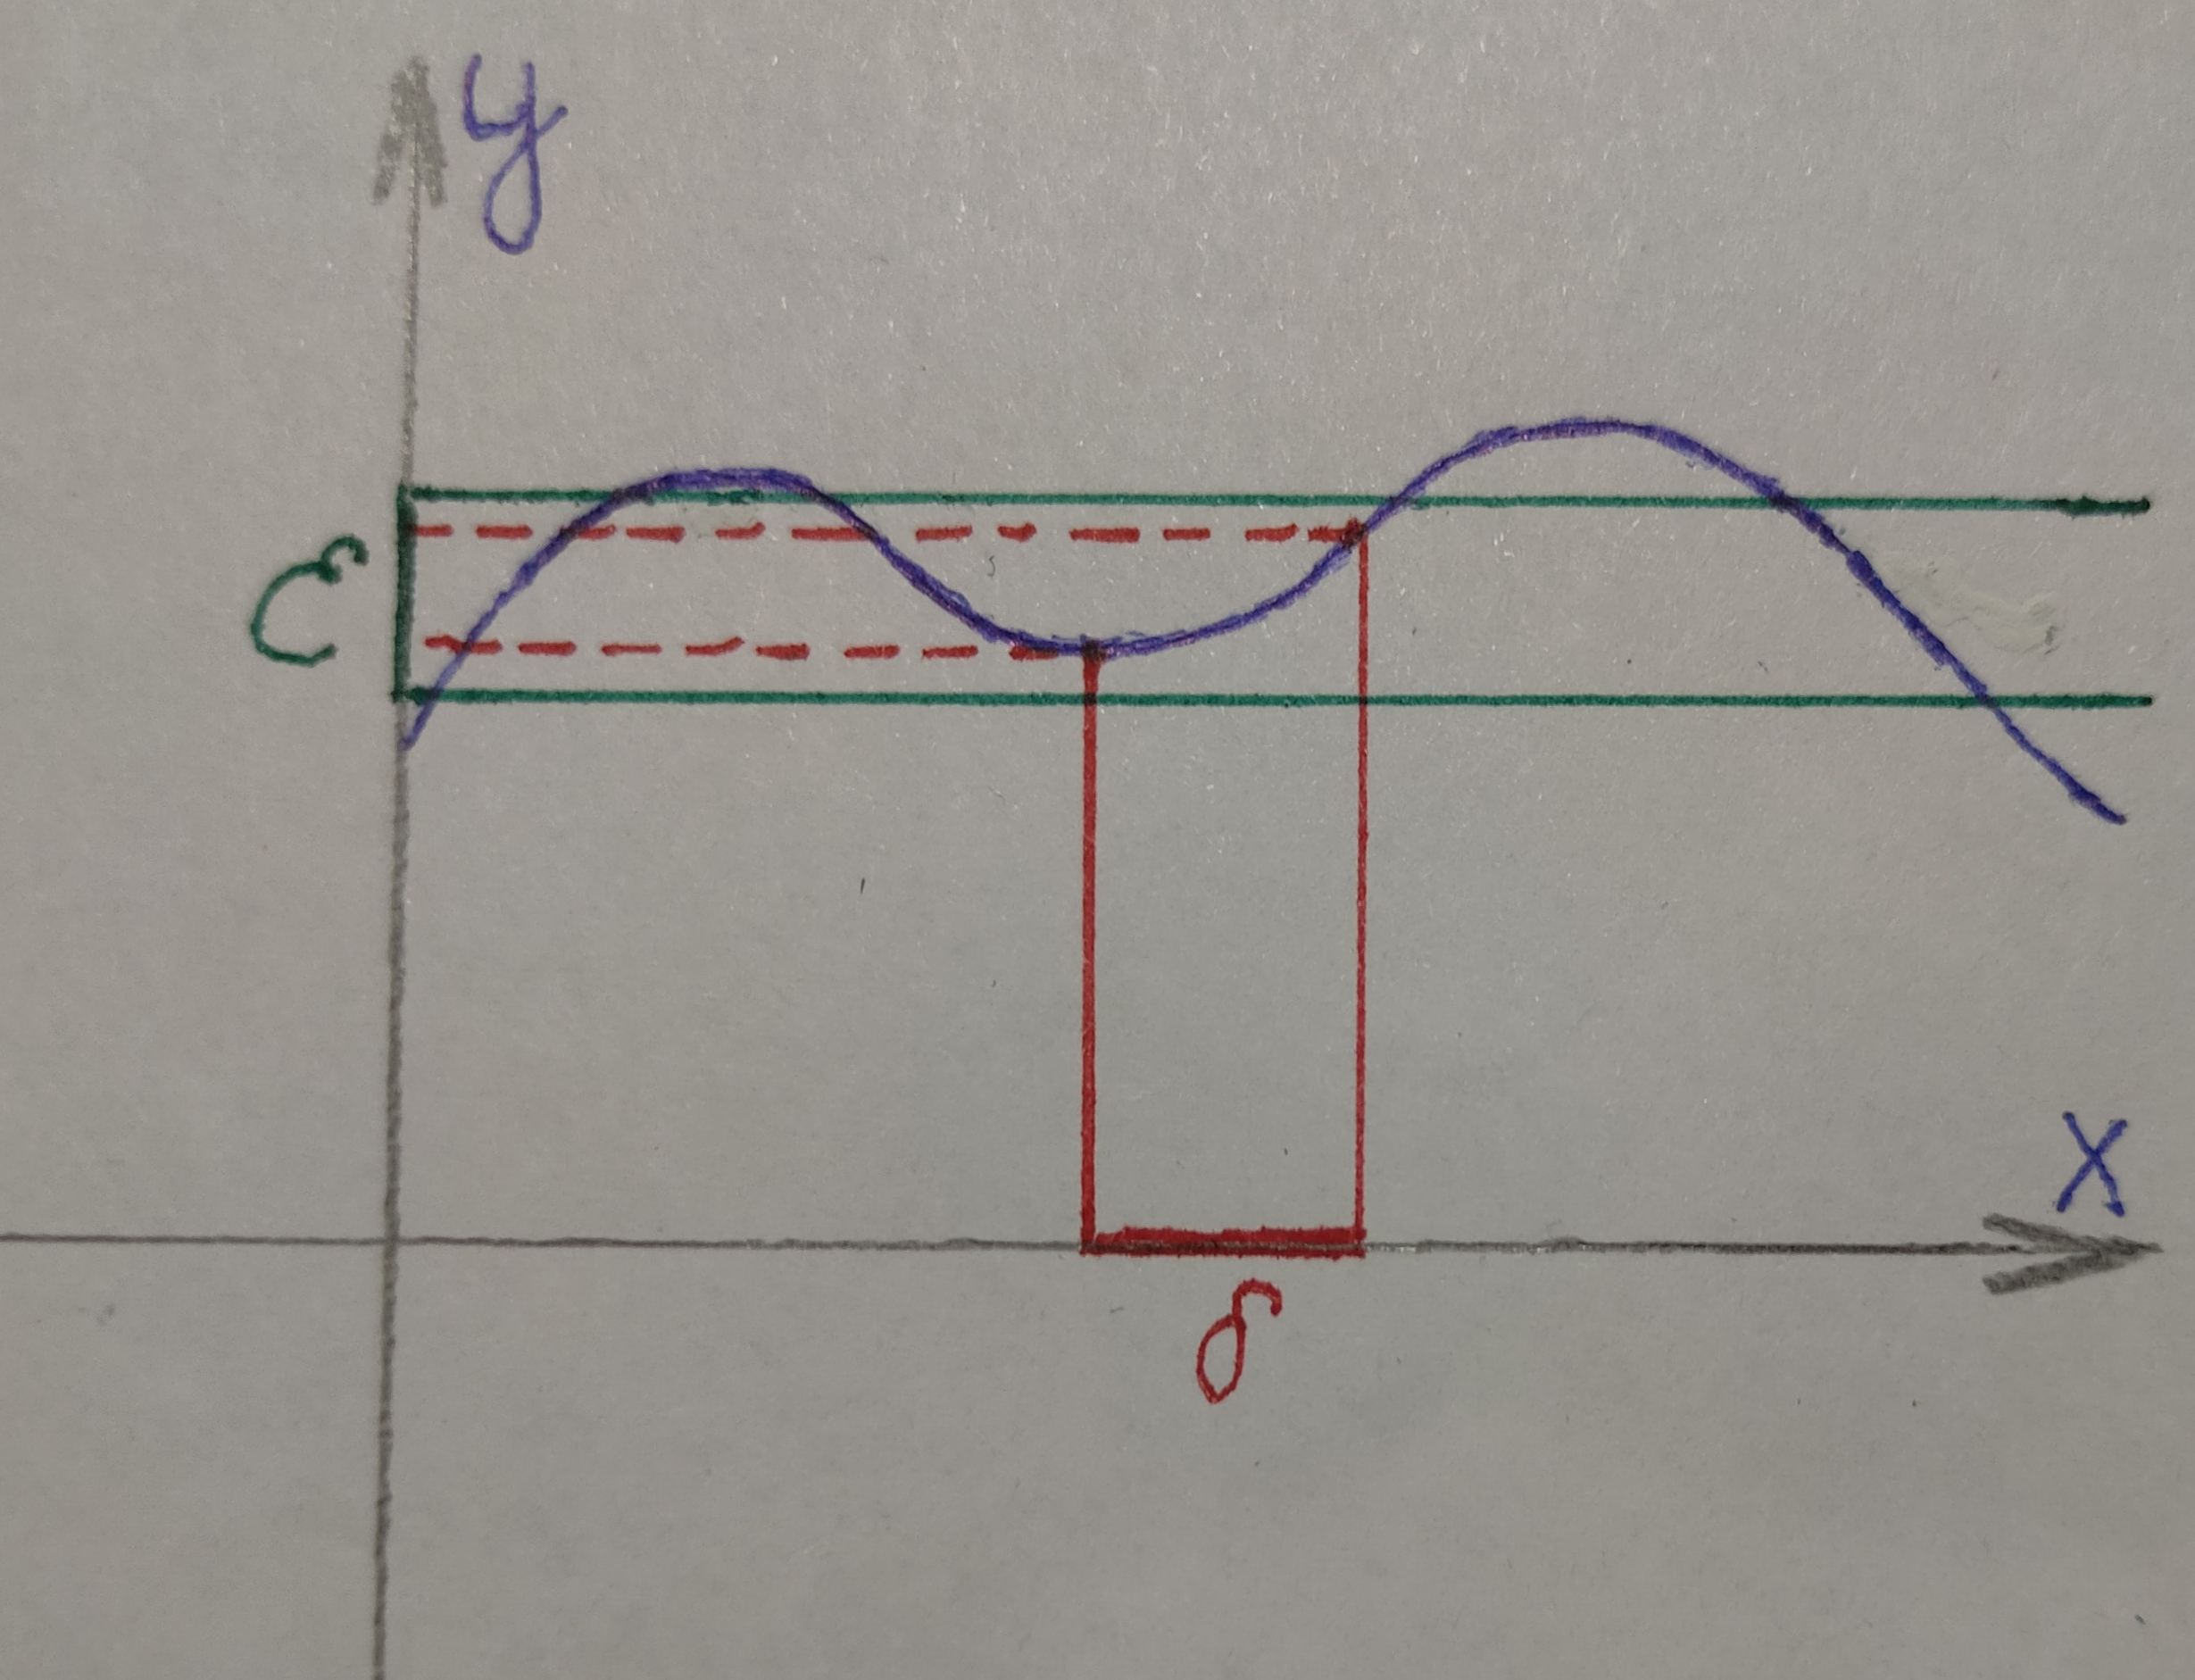
\includegraphics[width=0.5\textwidth]{img/lecture27/uniformly_continuous_function}
    \end{center}
    
    \begin{explanation}
    	Другими словами, существует $\delta$ на оси OX такая, что расстояние между $x$ и $y$ меньше, чем $\delta$, и разность между значениями функции в точках $x$ и $y$ помещается в этот $\epsilon-$корридор.
    \end{explanation}
    
    \begin{mention}
    	Если функция является равномерно-непрерывной, то она является и непрерывной, т. к. определение непрерывности слабее:
    	\[ f - \text{непрерывна на } X \Rightarrow \forall x_0 \in X \text{ } \forall \epsilon > 0 \text{ } \exists \delta > 0: \forall x \in B_{\delta}(x_0) \rightarrow |f(x) - f(x_0)| < \epsilon \]
    	
    	В обратную сторону это не правда, см. пункт 2) примера 10.12.
    \end{mention}
    
    \begin{example}
    	\begin{enumerate}
    		\item Функция $f(x) := \sin{x}$ равномерно непрерывна на $\R$, т.к.
    		по теореме Лагранжа $|\sin{x} - \sin{y}| = |\cos{\xi}| \cdot |x - y| \leqslant |x - y|$.
    		\item Функция $f(x) = \frac{1}{x}$ не равномерно непрерывна на $(0, 1)$,
    		т.к. $f(\frac{1}{2n}) - f(\frac{1}{n}) = n, а |\frac{1}{n} - \frac{1}{2n}| = \frac{1}{2n} \rightarrow 0$.
    	\end{enumerate}
    \end{example}
    
    \begin{explanation}
    	\begin{enumerate}
    		\item По теореме Лагранжа $\forall x, y \in \R |\sin{x} - \sin{y}| = |(\sin{\xi})'(x - y)| = |\cos{\xi}||(x - y)| \leqslant |x - y|$
    		\item Требуется доказать отрицание определения равномерной непрерывности:
    		\[ \exists \epsilon = 1 \text{ } \forall \delta > 0 \text{ } \exists x, y \in (0, 1) \text{ } |x - y| < \delta: |f(x) - f(y)| \geqslant 1 \]
    		Будем доказывать для $\delta = \frac{1}{n}$, потому что всегда можно взять $\frac{1}{n} < \delta$. Тогда пусть $x = x_n = \frac{1}{n}, y = y_n = \frac{1}{2n} \Rightarrow |x - y| = |\frac{1}{n} - \frac{1}{2n}| = \frac{1}{2n} < \frac{1}{n}, |f(x) - f(y)| = |n - 2n| = n \geqslant 1$.
    	\end{enumerate}
    \end{explanation}
    
    \section{Интегрируемость непрерывной функции}
    
    \begin{theorem}[Кантора]
    	Если функция $f$ непрерывна на отрезке $[a, b]$, то $f$ равномерно непрерывна на $[a, b]$.
    \end{theorem}
    
    \begin{proof}
    	Пусть $f$ - непрерывная функция на $[a, b]$, но не равномерно-непрерывная:
    	\[ \exists \epsilon > 0: \forall \delta = \frac{1}{n} > 0 \text{ } \exists x_n, y_n \in [a, b]: |x_n - y_n| < \frac{1}{n} \rightarrow |f(x_n) - f(y_n)| \geqslant \epsilon \]
    	$x_n$ - ограниченная последовательность, т. к. $x_n \in [a, b] \Rightarrow$ по теореме Больцано $\exists x_{n_k} \to x \Rightarrow$ из неравенства $|x_n - y_n| < \frac{1}{n}$ следует, что $x_{n_k} - \frac{1}{n} < y_{n_k} < x_{n_k} + \frac{1}{n}$.
    	$x_{n_k} - \frac{1}{n} \to x, x_{n_k} + \frac{1}{n} \to x \Rightarrow$ по теореме о зажатой последовательности $y_{n_k} \to x$.
    	\[ \epsilon \leqslant |f(x_{n_k}) - f(y_{n_k})| = |f(x_{n_k}) - f(x) + f(x) - f(y_{n_k})| \leqslant |f(x_{n_k}) - f(x)| + |f(x) - f(y_{n_k})| \]
    	Но $|f(x_{n_k}) - f(x)| \to 0, |f(x) - f(y_{n_k})| \to 0$, а $\epsilon > 0$ - противоречие.
    \end{proof}
    
    \begin{corollary}
    	Пусть $f$ непрерывна на $[a, b]$. Тогда $f$ интегрируема по Риману на $[a, b]$.
    \end{corollary}
    
    \begin{proof}
    	В силу предыдущей теоремы $f$ равномерно непрерывна на $[a, b]$. Поэтому 
    	\[ \forall \epsilon > 0 \text{ } \exists \delta > 0 : \forall T \text{ с } \Delta_T < \delta \text{ } \forall x, y \in \Delta_k \rightarrow \sup_{x, y \in \Delta_k} {|f(x) - f(y)|} < \epsilon \text{ } \forall k \Rightarrow \]
    	\[ \Rightarrow \omega(f, \Delta_k) < \epsilon \text{ } \forall k.\]
    	Для такого разбиения $\displaystyle \sum_{k = 1}^n \omega(f, \Delta_k) \Delta x_k < \epsilon |b - a| \Rightarrow$ по теореме 10.6 функция $f$ интегрируема по Риману на $[a, b]$.
    \end{proof}
    
    \section*{Лекция 28: Формула Ньютона-Лейбница}
    
    \section{Аддитивность интеграла}
    
    \begin{corollary}
    	Если $f$ интегрируема по Риману на отрезке $[a, b]$, $[c, d] \subseteq [a, b]$, то $f$ интегрируема на отрезке $[c, d]$.
    \end{corollary}
    
    \begin{proof}
    	$f$ - интегрируема на $[a, b] \Rightarrow$ по теореме 10.6 $\forall \epsilon > 0 \text{ } \exists T:$
    	\[ \sum_{k = 1}^n \omega(f, \Delta_k) \cdot \Delta x_k < \epsilon \Leftrightarrow 0 \leqslant \sum_{k = 1}^n \sup_{x \in \Delta_k} {f(x)} \cdot \Delta_k - \sum_{k = 1}^n \inf_{x \in \Delta_k} {f(x)} \cdot \Delta_k < \epsilon \Leftrightarrow \]
    	\[ \Leftrightarrow 0 \leqslant S(f, T) - s(f, T) < \epsilon \]
    	\begin{center}
    		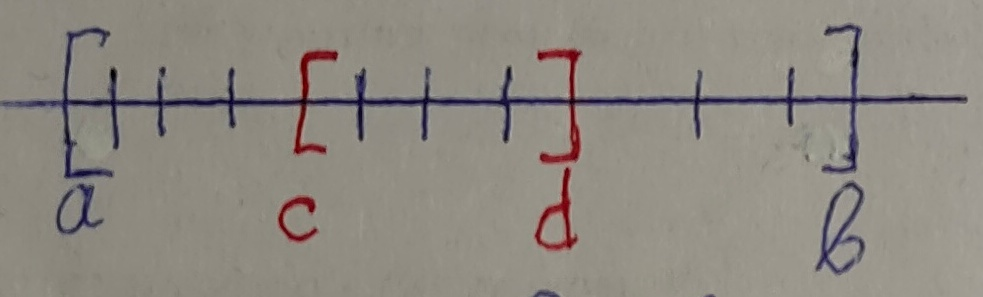
\includegraphics[width=0.2\textwidth]{img/lecture28/scheme_segments}
    	\end{center}
    	\begin{center}
    		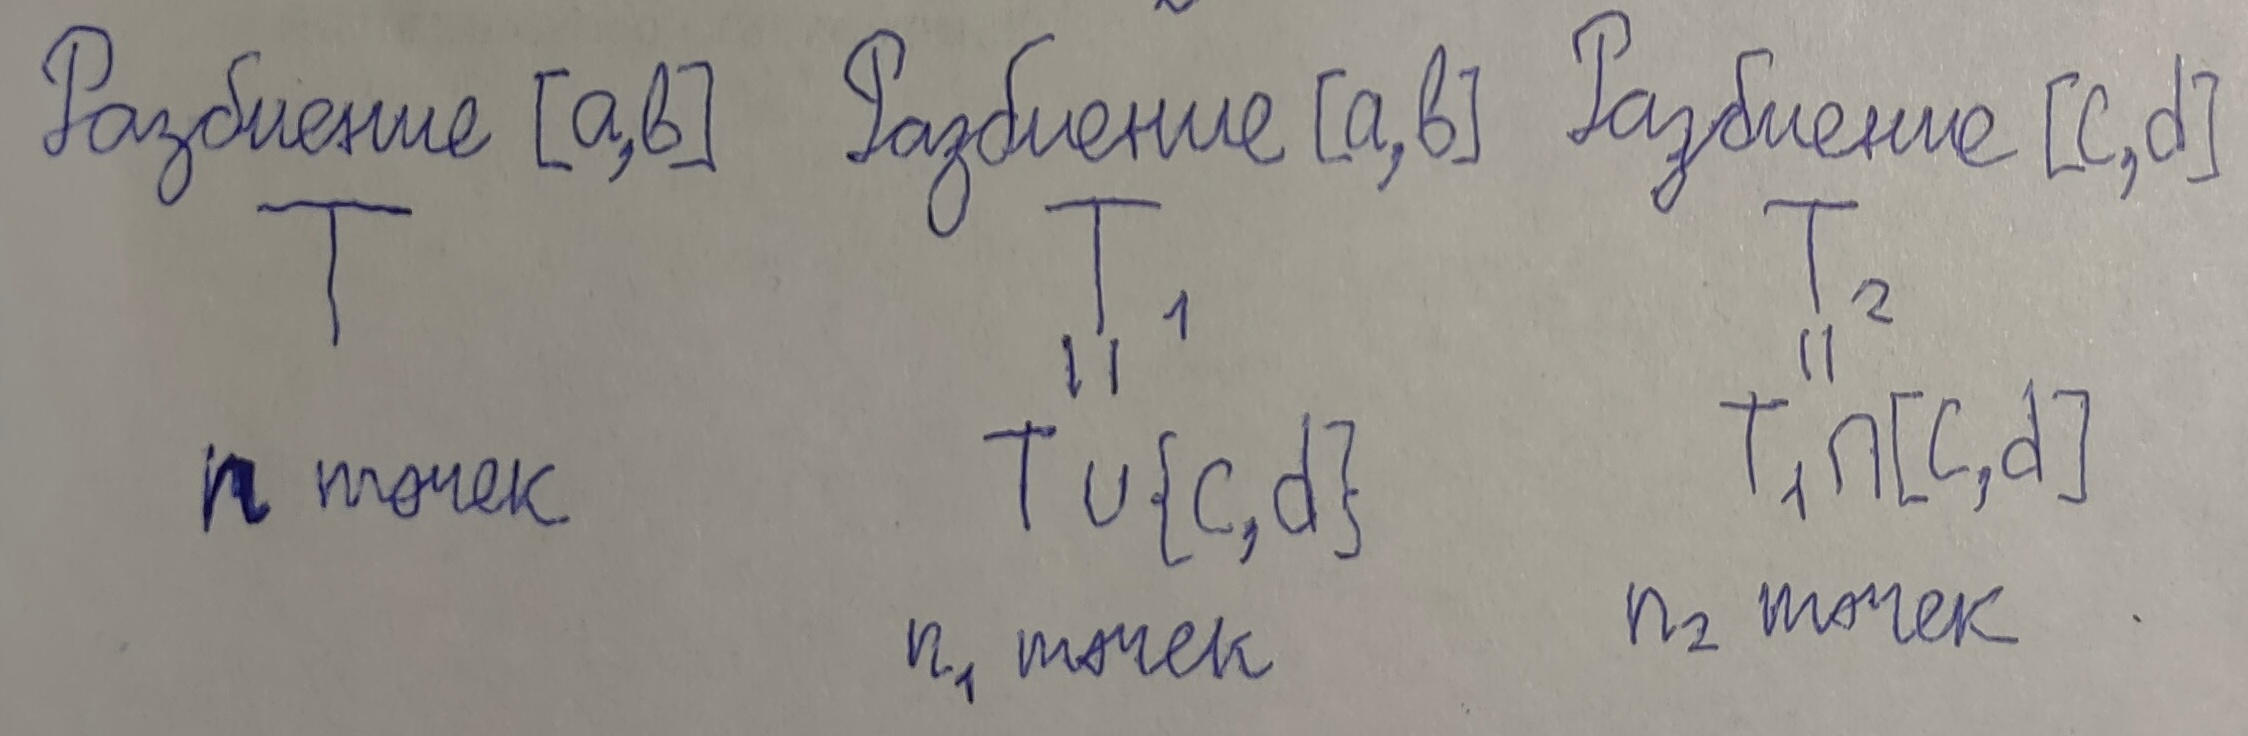
\includegraphics[width=0.5\textwidth]{img/lecture28/partition_designations}
    	\end{center}
    	\[ \sum_{k = 1}^{n_2} \omega(f, \Delta^2_k) \Delta^2 x_k \leqslant \sum_{k = 1}^{n_1} \omega(f, \Delta^1_k) \Delta^1 x_k \leqslant \sum_{k = 1}^n \omega(f, \Delta_k) \Delta x_k < \epsilon \]
    	
    	Первое неравенство выполняется, потому что в новую сумму мы добавили слагаемые отрезков, не входящих в отрезок $[c, d]$, но принадлежащих отрезку $[a, b]$, колебание функции всегда неотрицательно (разность супремума и инфимума функции неотрицательна). Здесь мы переходим от разбиения $T_2$ к разбиению $T_1$. Второе неравенство выполняется, потому что $T_1$ - это измельчение разбиения $T$. На измельчении нижняя сумма Дарбу $s(f, T_1)$ только больше, а верхняя сумма Дарбу $S(f, T_1)$ только меньше, значит разность $S(f, T_1) - s(f, T_1) \leqslant S(f, T) - s(f, T)$ (лемма 10.2, пункт 2).
    \end{proof}
    
    \begin{corollary}
    	Если $f$ интегрируема по Риману на отрезке $[a, b]$, $c \in [a, b]$, то $f$ интегрируема на отрезках $[a, c]$ и $[c, b]$ и верно равенство
    	\[ \int_a^b f(x) \; dx = \int_a^c f(x) \; dx + \int_c^b f(x) \; dx. \]
    \end{corollary}
    
    \begin{proof}
    	Если интеграл слева существует, то существуют и интегралы cправа по предыдущему следствию (на самом деле утверждение верно в обратную сторону, но доказательство на лекциях не приводилось).
    	
    	\begin{mention}
    		Если $f$ - интегрируема на $[a, b]$, то для любой последовательности разбиений $T_n$ такой, что $\Delta_{T_n} \to 0$, интегральное разбиение $\sigma(f, T_n, \xi_n) \to I$.
    	\end{mention}
    	\begin{proof}
    		$f$ - интегрируема на $[a, b] \Rightarrow$ по определению $\forall \epsilon > 0 \text{ } \exists \delta > 0: \forall T$ с $\Delta_T < \delta$ и $\xi \rightarrow |\sigma(f, T_n, \xi_n) - I| < \epsilon$
    		
    		Тогда
    		\[ \forall \epsilon > 0 \text{ } \exists N: \forall n > N \text{ } \Delta_{T_n} < \delta \rightarrow |\sigma(f, T_n, \xi_n) - I| < \epsilon \Rightarrow \sigma(f, T_n, \xi_n) \rightarrow I \]
    	\end{proof}
    	
    	Это означает, что если функция интегрируемая, то можно выбирать любое разбиение, с стремящимся к нулю диаметром, чтобы найти интеграл.
    	
    	Будем брать такое разбиение $T$ отрезка $[a, b]$, которые содержат точку $c$. $T_1$ - разбиение отрезка $[a, c]$, $T_2$ - разбиение отрезка $[c, b]$.
    	\begin{center}
    		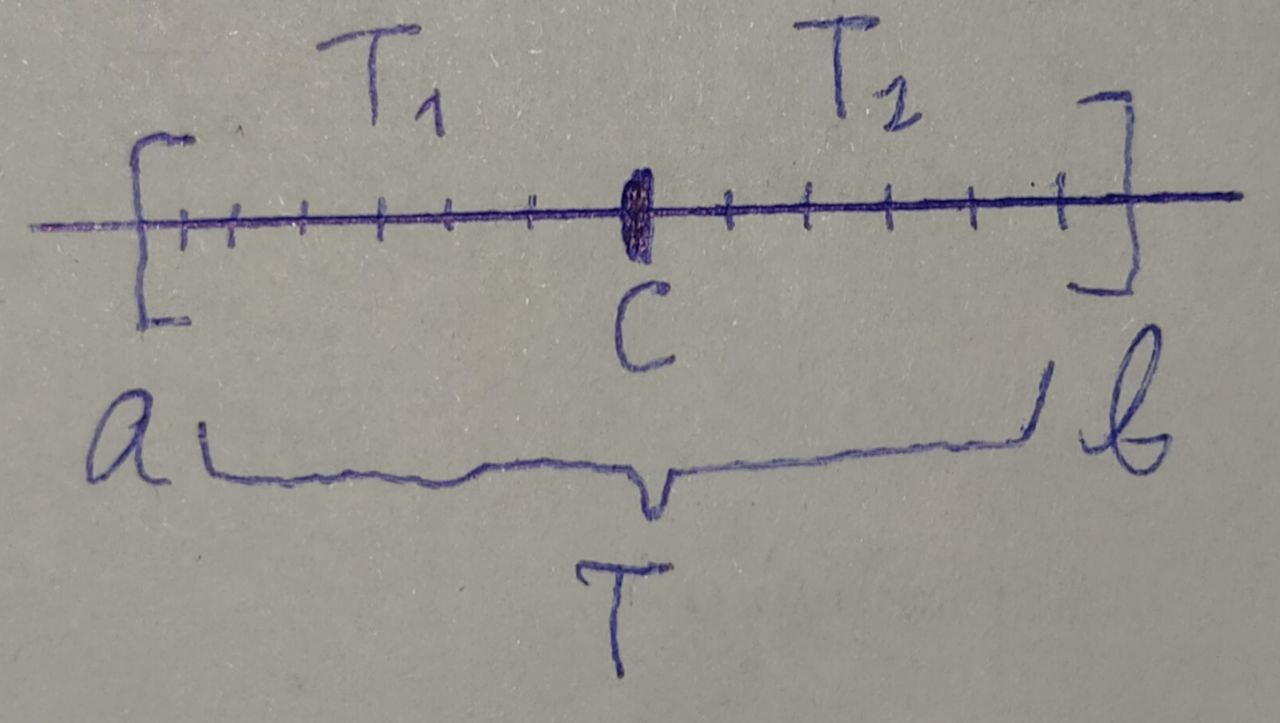
\includegraphics[width=0.3\textwidth]{img/lecture28/partition_with_c_dot}
    	\end{center}
    	
    	$f$ - интегрируема $\Rightarrow \forall \epsilon > 0 \text{ } \exists \delta > 0: \forall T \text{ с } \Delta_T < \delta \rightarrow |\sigma(f, T, \xi) - I| < \epsilon$
    	
    	$\Delta_T < \delta \Rightarrow \Delta_{T_1} < \delta, \Delta_{T_2} < \delta \Rightarrow |\sigma(f, T_1, \xi_1) - I_1| < \epsilon, |\sigma(f, T_2, \xi_2) - I_2| < \epsilon$
    	
    	Пусть отрезок $[a, c]$ поделен на $n_1$ отрезков. Тогда    	
    	\[ \sigma(f, T, \xi) = \sum_{k = 1}^n f(\xi_k) \Delta x_k = \sum_{k = 1}^{n_1} f(\xi_k) \Delta x_k + \sum_{k = n_1 + 1}^n f(\xi_k) \Delta x_k = \sigma(f, T_1, \xi_1) + \sigma(f, T_2, \xi_2) \Rightarrow \]
    	\[ \Rightarrow |\sigma(f, T, \xi) - I_1 - I_2| = |\sigma(f, T_1, \xi_1) + \sigma(f, T_2, \xi_2) - I_1 - I_2| \leqslant \]
    	\[ \leqslant |\sigma(f, T_1, \xi_1) - I_1| + |\sigma(f, T_2, \xi_2) - I_2| < 2\epsilon \]
    	Следовательно,
    	\[ \sigma(f, T, \xi) \to I, \sigma(f, T, \xi) \to I_1 + I_2 \Rightarrow I_1 + I_2 = I \]
    \end{proof}
    
    \section{Формула Ньютона–Лейбница}
    
    \begin{theorem}[Формула Ньютона–Лейбница]
    	Пусть $F$ - первообразная интегрируемой по Риману на отрезке
    	$[a, b]$ функции $f$. Тогда
    	\[ \int_{a}^{b} f(x) \; dx = F(b) - F(a) = F(x)\bigg|_{a}^{b}. \]
    \end{theorem}
    
    \begin{proof}
    	Рассмотрим разбиение $T$ отрезка $[a, b]$.
    	\begin{center}
    		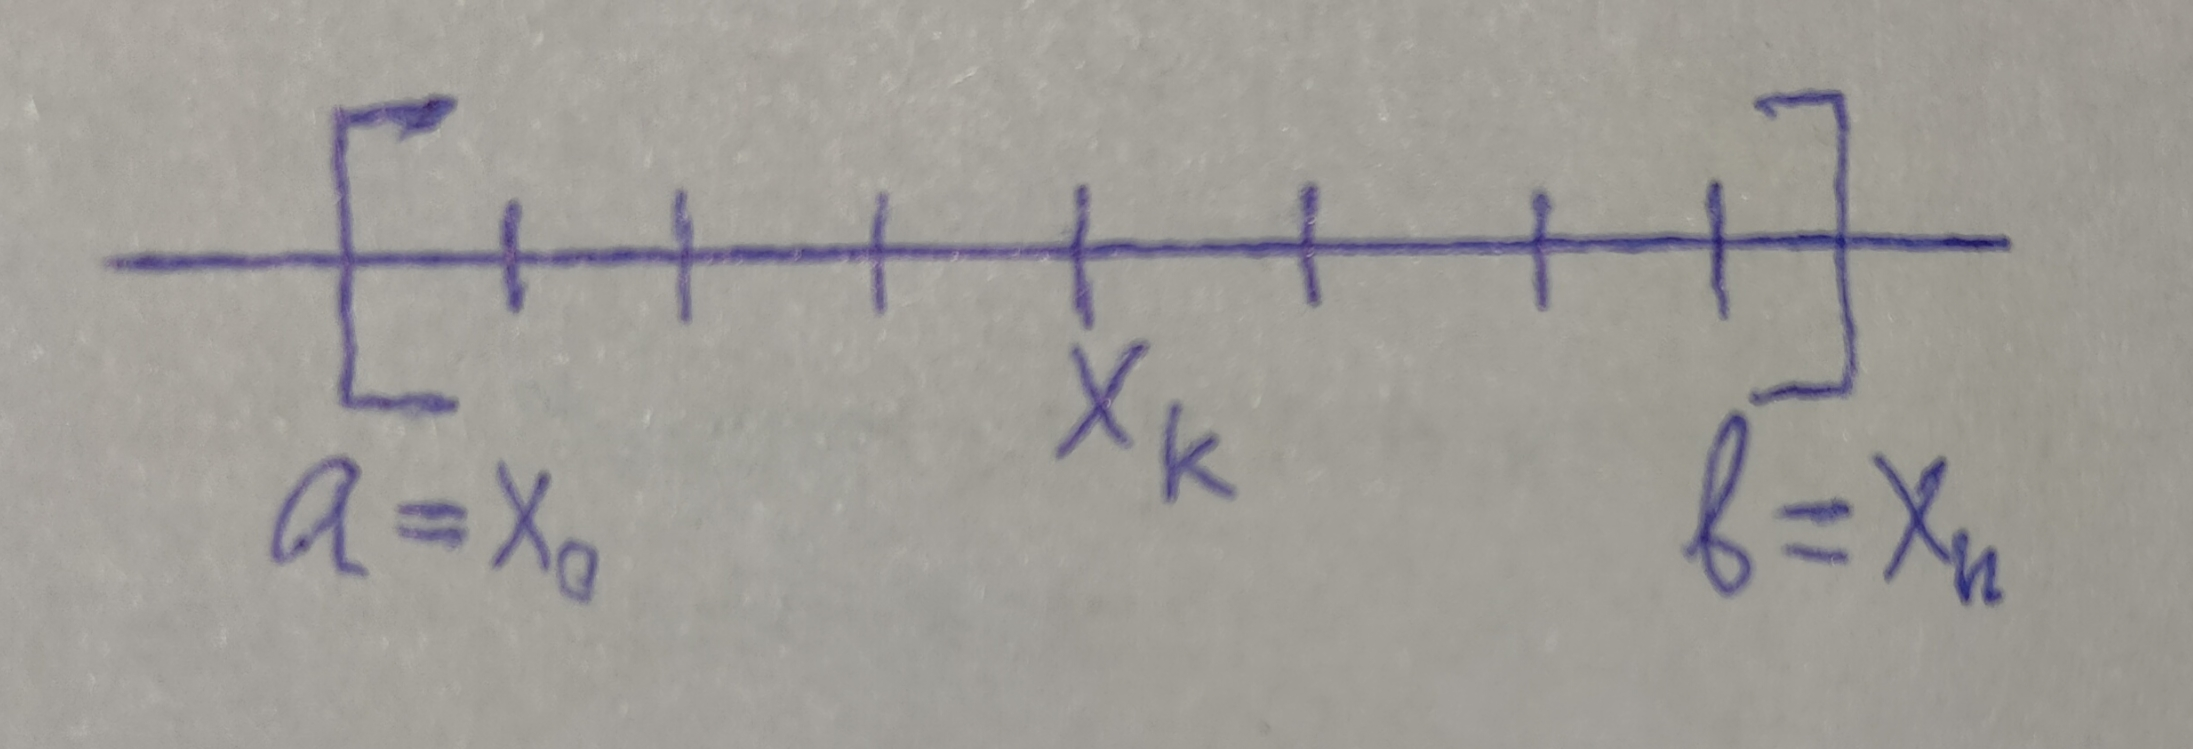
\includegraphics[width=0.3\textwidth]{img/lecture28/Newton_Leibniz_theorem}
    	\end{center}
    	\[ F(b) - F(a) = F(x_1) - F(x_0) + F(x_2) - F(x_1) + F(x_3) - F(x_2) + ... \]
    	\[ ... + F(x_n) - F(x_{n - 1}) = \sum_{k = 1}^n F(x_k) - F(x_{k - 1}) = (*) \]
    	Применяем теорему Лагранжа для каждого отрезка $[x_{k - 1}, x_k]$:
    	\[ (*) = \sum_{k = 1}^n F'(\xi_k) \Delta x_k = \sum_{k = 1}^n f(\xi_k) \Delta x_k = \sigma(f, T, \xi) \]
    	Число $F(b) - F(a)$ равняется интегральной сумме Римана $\sigma(f, T, \xi)$. Поскольку функция интегрируема, то по замечанию из следствия выше при $T \to 0$ интегральная сумма Римана стремится к интегралу $\int_{a}^{b} f(x) \; dx$. При этом, как мы показали, для любого разбиения $T$ всегда есть такая разметка $\xi$, когда $F(b) - F(a) = \sigma(f, T, \xi)$. Тогда
    	\[ \int_{a}^{b} f(x) \; dx = F(b) - F(a) \]
    \end{proof}
    
    Далее будем использовать соглашение: при $b > a$ по
    определению 
    \[ \displaystyle\int_{b}^{a} f(x) \; dx = -\displaystyle\int_{a}^{b} f(x) \; dx.\]
    
    \section{Существование первообразной}
    
    \begin{theorem}
    	Пусть $f$ интегрируема по Риману на $[a, b]$. Тогда функция
    	\[ F(x) := \int_a^{x} f(x) \; dx \]
    	непрерывна на $[a, b]$. Кроме того, если $f$ непрерывна в точке
    	$x_0 \in [a, b]$, то $F$ дифференцируема в $x_0$ и $F'(x_0) = f(x_0)$.
    \end{theorem}
    
    \begin{proof}
    	Доказательство первого утверждения.
    	
    	$y \in [a, b]$    	
    	\[ F(y) = \int_a^y f(x) \; dx \]
    	\[ |F(y) - F(x_0)| = \bigg| \int_a^y f(x) \; dx - \int_a^{x_0} f(x) \; dx \bigg| =  \bigg| \int_{x_0}^y f(x) \; dx \bigg| \]
    	$f$ - интегрируема на $[a, b] \Rightarrow$ ограничена: $|f(x)| \leqslant M$
    	\[  \bigg| \int_{x_0}^y f(x) \; dx  \bigg| \leqslant  \bigg| \int_{x_0}^y M \; dx  \bigg| = M \cdot |y - x_0| \Rightarrow \]
    	$\Rightarrow$ при $y \to x_0$ $F(y) \to F(x_0) \Rightarrow F(x)$ непрерывна.
    	
    	Доказательство второго утверждения.
    	
    	Пусть теперь $f$ непрерывна в $x_0 \Rightarrow \forall \epsilon > 0 \text{ } \exists \delta > 0: \forall x \in B_{\delta}(x_0) \rightarrow |f(x) - f(x_0)| < \epsilon$
    	\[ f(x_0) - \epsilon \leqslant f(x) \leqslant f(x_0) + \epsilon \]
    	Воспользуемся монотонностью интеграла и проинтегрируем каждую часть.
    	\[ \int_{x_0}^x (f(x_0) - \epsilon) \; dx \leqslant \int_{x_0}^x f(x) \; dx \leqslant \int_{x_0}^x (f(x_0) + \epsilon) \; dx \]
    	\[ (f(x_0) - \epsilon)(x - x_0) \leqslant F(x) - F(x_0) \leqslant (f(x_0) + \epsilon)(x - x_0) \]
    	Пусть $x > x_0$, поделим на $x - x_0$.
    	\[ f(x_0) - \epsilon \leqslant \frac{F(x) - F(x_0)}{x - x_0} \leqslant f(x_0) + \epsilon \Rightarrow \bigg| \frac{F(x) - F(x_0)}{x - x_0} - f(x_0) \bigg| < \epsilon \]
    	Это означает, что предел $\lim_{x \to x_0} \frac{F(x) - F(x_0)}{x - x_0}$ существует и он равен $f(x_0)$. Таким образом, $F$ дифференцируема в $x_0$ и $F'(x_0) = f(x_0)$.
    	
    	Если $x < x_0$, то когда поделим на $x - x_0$ знаки перевернутся, но в итоге мы получим тоже самое.
    \end{proof}
    
    \begin{corollary}
    	Пусть $f$ непрерывна на $[a, b]$, тогда у $f$ существует первообразная.
    \end{corollary}
    
    \begin{explanation}
    	Если во всех точках $f$ непрерывна, то по теореме 10.19 первообразная $f$ существует во всех точках.
    \end{explanation}
    
    \section{Формула интегрирования по частям}
    
    \begin{theorem}[Формула интегрирования по частям]
    	Пусть $f$, $g$ — непрерывно дифференцируемые на отрезке $[a, b]$ функции. Тогда
    	\[ \int_a^b f(x)g'(x) \; dx = f(b)g(b) - f(a)g(a) - \int_a^b f'(x)g(x) \; dx. \]
    \end{theorem}
    
    \begin{proof}
    	$F(x) = g(x) \cdot f(x)$
    	
    	$F'(x) = g'(x) \cdot f(x) + g(x) \cdot f'(x)$
    	
    	Непрерывно дифференцируемая функция - это дифференцируемая функция, у которой первая производная непрерывна. Это означает, что $g'(x) \cdot f(x)$ и $g(x) \cdot f'(x)$ непрерывны $\Rightarrow g'(x) \cdot f(x) + g(x) \cdot f'(x)$ непрерывна. У непрерывных функций есть первообразная по предыдущему следствию. Тогда мы можем их интегрировать.
    	
    	$\int_a^b F'(x) \; dx = F(b) - F(a)$    	
    	\[ g(b) \cdot f(b) - g(a) \cdot f(a) = F(b) - F(a) = \int_a^b F'(x) \; dx = \int_a^b g'(x) \cdot f(x) + g(x) \cdot f'(x) \; dx = \]
    	\[ = \int_a^b g'(x) \cdot f(x) \; dx + \int_a^b g(x) \cdot f'(x) \; dx \]
    \end{proof}
    
    \begin{example}
    	$\displaystyle\int_0^1 \arctg{x} \; dx.$
    \end{example}
    \[ \displaystyle\int_0^1 \arctg{x} \; dx = x\arctg{x}\bigg|_0^1 - \int_0^1 x \; d\arctg{x} = \frac{\pi}{4} - \int_0^1 \frac{x}{1 + x^2} \; dx = \frac{\pi}{4} - \frac{1}{2} \int_0^1 \frac{d(1 + x^2)}{1 + x^2} = \]
    \[ = \frac{\pi}{4} - \frac{1}{2} \ln{|x^2 + 1|} \bigg|_0^1 = \frac{\pi}{4} - \frac{\ln{2}}{2} \]
    
    \chapter{Критерий Дарбу и классы интегрируемых функций}
    
    \section*{Лекция 29: Несобственный интеграл}
    
    \section{Формула интегрирования подстановкой}
    
    \begin{theorem}
    	Пусть $f$ — непрерывна на $[a, b], \phi: [\alpha, \beta] \rightarrow [a, b]$ — непрерывно дифференцируемая функция. Тогда
    	\[ \int_{\phi(\alpha)}^{\phi(\beta)} f(x) \; dx = \int_{\alpha}^{\beta} f(\phi(t))\phi'(t) \; dt. \]
    \end{theorem}
    
    \begin{proof}
    	$f$ — непрерывна на $[a, b] \Rightarrow f$ - интегрируема на $[\phi(a), \phi(b)]$ (функция интегрируема на любом подотрезке $[a, b]$) и у $f$ есть первообразная (по теореме 10.19).
    	
    	Тогда у функции $f(\phi(t))\phi'(t)$ тоже есть первообразная $F(\phi(t))$.
    	
    	\[ \int_{\alpha}^{\beta} f(\phi(t))\phi'(t) = F(\phi(\beta)) - F(\phi(\alpha)) = \int_{\phi(\alpha)}^{\phi{(\beta)}} f(x) \; dx \]
    \end{proof}
    
    \begin{example}
    	$\displaystyle\int_0^{\frac{\pi}{4}} \frac{1}{1 + \cos^2{x}} \; dx.$
    \end{example}
    
    \[ \int_0^{\frac{\pi}{4}} \frac{1}{1 + \cos^2{x}} \; dx = \int_0^{\frac{\pi}{4}} \frac{\frac{1}{\cos^2{x}}}{\frac{1}{\cos^2{x}} + 1} \; dx = (*) \]
    
    \[ \sin^2{x} + \cos^2{x} = 1 \Rightarrow \tg^2{x} + 1 = \frac{1}{\cos^2{x}} \Rightarrow \tg^2{x} = \frac{1}{\cos^2{x}} - 1 \]
    
    Применяем формулу
    \[ (*) = \int_0^{\frac{\pi}{4}} \frac{d\tg{x}}{\tg^2{x} + 2} = \int_{\tg{0}}^{\tg{\frac{\pi}{4}}} \frac{dy}{y^2 + 2} = \int_0^1 \frac{dy}{y^2 + 2} = \frac{1}{\sqrt{2}} \arctg{\frac{y}{\sqrt{2}}} \bigg|_0^1 = \frac{1}{\sqrt{2}} \arctg{\frac{1}{\sqrt{2}}} \]
    
    \section{Мера Жордана (дополнительный материал)}
    Пусть $\Delta$ — параллелепипед в $\R^n$, являющийся декартовым произведением промежутков вида $[a_i, b_i]$, $(a_i, b_i)$, $[a_i, b_i)$ или $(a_i, b_i]$. Мера Жордана параллелепипеда $\Delta$ определяется как
    произведение
    \[ \mu\Delta = \prod_{i = 1}^{n} (b_i - a_i). \]
    
    Для ограниченного множества $E \subset \R^n$ определяются:
    \begin{itemize}
    	\item внешняя мера Жордана
    	\[ \mu^{*}E = \inf{\sum_{k = 1}^{N} \mu \Delta_k}, \text{   } \bigcup_k{\Delta_k} \supset E \]
    	\item внутренняя мера Жордана
    	\[ \mu_{*}E = \sup{\sum_{k = 1}^{N} \mu \Delta_k}, \bigcup_k{\Delta_k} \subset E, \Delta_k \cap \Delta_m = \varnothing, \text{ если } k \neq m. \]
    \end{itemize}
    
    Здесь $\Delta_1, \Delta_2, ..., \Delta_N$ — параллелепипеды описанного выше вида.
    
    \begin{definition}
    	Множество $E$ называется измеримым по Жордану (или
    	квадрируемым), если $\mu^{*}E = \mu_{*}E$. В этом случае мера Жордана равна $\mu E = \mu^{*}E = \mu_{*}E$.
    \end{definition}
    
    \section{Несобственный интеграл Римана}
    
    \begin{definition}
    	Пусть $f$ интегрируема на каждом отрезке $[a, x]$ при $x < b$ $(b \in (-\infty, +\infty])$. Говорят, что несобственный интеграл
    	\[ \int_a^b f(t) \; dt \]
    	\underline{сходится}, если существует предел
    	\[ \lim_{x \to b - 0} \int_a^x f(t) \; dt. \]
    
	    В этом случае значение несобственного интеграла полагают равным значению данного предела. В противном случае (если предела не существует) говорят, что несобственный интеграл \underline{расходится}.
	    
	    Аналогично определяется несобственный интеграл с особенностью в нижнем пределе интегрирования.
	\end{definition}
	
	\begin{example}
	    \begin{equation*}
	    	\int_1^b \frac{1}{x^p} \; dt = 
		    \begin{cases}
		    	\frac{1}{1 - p}(b^{1 - p} - 1), & p \neq 1, \\
		    	\ln{b}, & p = 1.
		    \end{cases}
	    \end{equation*}
	    
	    Предел при $b \rightarrow \infty$ существует тогда и только тогда, когда $p > 1$.
	    
	    С другой стороны,
	    \begin{equation*}
	    	\int_b^1 \frac{1}{x^p} \; dt = 
	    	\begin{cases}
	    		\frac{1}{1 - p}(1 - b^{1 - p}), & p \neq 1, \\
	    		-\ln{b}, & p = 1.
	    	\end{cases}
	    \end{equation*}
	    
	    Предел при $b \rightarrow 0$ существует тогда и только тогда, когда $p < 1$.
	\end{example}
	
	\section{Свойства несобственного интеграла}
	
	\begin{theorem}
		Пусть $f$, $g$ интегрируемы на каждом отрезке $[a, x]$ при $x < b$ и пусть для них определены несобственные интегралы на
		промежутке $[a, b)$. Тогда
		\begin{enumerate}
			\item если $b \in \R$ и $f$ интегрируема на $[a, b]$, то значение несобственного интеграла на промежутке $[a, b)$ совпадает со значением обычного интеграла Римана по отрезку $[a, b]$;
			\item функция $\alpha f + \beta g$ интегрируема в несобственном смысле на промежутке $[a, b)$ и
			\[ \int_a^b (\alpha f + \beta g) \; dx = \alpha \int_a^b f(x) \; dx + \beta \int_a^b g(x) \; dx; \]
			\item если $c \in [a, b)$, то
			\[ \int_a^b f(x) \; dx = \int_a^c f(x) \; dx + \int_c^b f(x) \; dx; \]
		\end{enumerate}
	\end{theorem}
	
	\begin{proof}
		\begin{enumerate}
			\item По определению $\int_a^b f(x) \; dx = \lim_{t \to b-} \int_a^t f(x) \; dx$.
			
			По теореме 10.19 если $F(t) = \int_a^t f(x) \; dx$ интегрируема на $[a, b]$, то $F(t)$ непрерывна на $[a, b] \Rightarrow \lim_{t \to b-} \int_a^t f(x) \; dx = F(b) = \int_a^b f(x) \; dx$.
			\item $\int_a^b \alpha f(x) + \beta g(x) \; dx = \lim_{t \to b-} \int_a^t \alpha f(x) + \beta g(x) \; dx \text{ (здесь уже обычный опреде-}$
			
			$\text{лённый интеграл, применяем линейность)} = \lim_{t \to b-} \alpha \int_a^t f(x) \; dx + \beta \int_a^t g(x) \; dx = \alpha \lim_{t \to b-} \int_a^t f(x) \; dx + \beta \lim_{t \to b-} \int_a^t g(x) \; dx = \alpha \int_a^b f(x) \; dx + \beta \int_a^b g(x) \; dx$
			
			Мы предполагаем, что интегралы $\int_a^b f(x) \; dx$ и $\int_a^b g(x) \; dx$ существуют, тогда существует интеграл  $\int_a^b \alpha f(x) + \beta g(x) \; dx$.
			\item $\int_a^b f(x) \; dx = \lim_{t \to b-} \int_a^t f(x) \; dx = (*)$
			
			При $c \in [a, b)$ для уже определённого интеграла применяем аддитивность:
			
			$(*) = \lim_{t \to b-} \int_a^c f(x) \; dx + \int_c^t f(x) \; dx = \int_a^c f(x) \; dx + \lim_{t \to b-} \int_c^t f(x) \; dx = \int_a^c f(x) \; dx + \int_c^b f(x) \; dx.$
			
			В отличие от пункта 2 здесь равенство выполняется в обе стороны: $\int_a^c f(x) \; dx$ является константой, поэтому предел $\lim_{t \to b-} \int_c^t f(x) \; dx$ существует тогда и только тогда, когда существует $\lim_{t \to b-} \int_a^t f(x) \; dx$.
		\end{enumerate}
	\end{proof}
	
	\section{Формула интегрирования подстановкой}
	
	\begin{theorem}
		Пусть $f$ непрерывна на $[a, b)$ и интегрируема в несобственном смысле, $\phi: [\alpha, \beta) \rightarrow [a, b)$ - непрерывно дифференцируемое отображение, $\phi(\alpha) = a, \phi(t) \rightarrow b$ при $t \rightarrow \beta$. Тогда функция $t \mapsto f(\phi(t))\phi'(t)$ интегрируема в несобственном смысле на промежутке $[\alpha, \beta)$ и
		\[ \int_a^b f(x) \; dx = \int_{\alpha}^{\beta} f(\phi(t))\phi'(t) \; dt. \]
	\end{theorem}
	
	\begin{proof}
		Из условия теоремы знаем, что
		\[ \exists \int_a^b f(x) \; dx = \lim_{y \to b-} \int_a^y f(x) \; dx\]
		
		Рассмотрим следующий интеграл (мы не знаем заранее, существует ли он):
		\[ \int_{\alpha}^{\beta} f(\phi(t)) \phi'(t)\; dt = \lim_{s \to \beta} \int_{\alpha}^s f(\phi(t))\phi'(t) \; dt \]
		
		При этом не важно с какой стороны $s$ стремится к $\beta$ (справа или слева), потому что мы определили интеграл как в случае $\alpha < \beta$, так и в случае $\beta < \alpha$.
		
		Для данного определённого интеграла под пределом действует формула интегрирования заменой (теорема 11.1).
		
		\[ \lim_{s \to \beta} \int_{\alpha}^s f(\phi(t))\phi'(t) \; dt = \lim_{s \to \beta} \int_{\phi(\alpha)}^{\phi(s)} f(x) \; dx \]
		
		$\phi(\alpha) = a, \phi(s) \to b$ при $s \to \beta \Rightarrow$
		\[ \lim_{s \to \beta} \int_{\phi(\alpha)}^{\phi(s)} f(x) \; dx = \lim_{y \to b} \int_a^y f(x) \; dx \]
		что тоже самое, что интеграл в начале доказательства. Значит интеграл $\int_{\alpha}^{\beta} f(\phi(t)) \phi'(t)$ существует и равен $\int_a^b f(x) \; dx$.
	\end{proof}
	
	\section{Формула интегрирования по частям}
	
	\begin{theorem}
		Пусть $f, g$ непрерывно дифференцируемы на $[a, b)$ и существует предел $\displaystyle\lim_{x \to b - 0} f(x)g(x)$. Тогда функции $f'g$ и $fg'$ одновременно интегрируемы или не интегрируемы в несобственном смысле на $[a, b)$ и в случае интегрируемости
		\[ \int_a^b f(t)g'(t) \; dt = \lim_{x \to b - 0} f(x)g(x) - f(a)g(a) - \int_a^b f'(t)g(t) \; dt. \]
	\end{theorem}
	
	\begin{proof}
		Если существует $\displaystyle\lim_{x \to b - 0} f(x)g(x)$, то $\displaystyle\lim_{x \to b - 0} f(x)g(x) - f(a)g(a)$ - это число. Тогда функции $f'g$ и $fg'$ одновременно интегрируемы или не интегрируемы в несобственном смысле на $[a, b)$.
		
		В случае интегрируемости
		\[ \int_a^b f(t)g'(t) \; dt = \lim_{x \to b} \int_a^x f(t)g'(t) \; dt \]
		Применяем формулу интегрирования по частям для определённого интеграла
		\[ \lim_{x \to b} \int_a^x f(t)g'(t) \; dt = \lim_{x \to b-} \bigg(f(x)g(x) - f(a)g(a) - \int_a^x f'(t)g(t) \; dt \bigg) = \]
		\[ = \lim_{x \to b-} f(x)g(x) - f(a)g(a) - \int_a^b f'(t)g(t) \; dt \]
	\end{proof}
	
	\section{Критерий Коши}
	
	\begin{theorem}[Критерий Коши]
		Пусть функция $f(x)$ определена на промежутке $[a; b)$,
		интегрируема в собственном смысле на любом отрезке
		$[a; \xi] \subseteq [a; b)$ и неограниченна в левой окрестности точки $x = b$. Тогда для сходимости интеграла
		\[ \int_a^b f(x) \; dx \]
		необходимо и достаточно, чтобы для любого числа $\epsilon > 0$
		существовало такое число $\eta$, что при любых $\eta_1, \eta_2 \in (\eta; b)$
		\[ \bigg| \int_{\eta_1}^{\eta_2} f(x) \; dx \bigg| < \epsilon. \]
	\end{theorem}
	
	\begin{proof}
		Запишем критерий Коши для функции $F(x) = \int_a^x f(t) \; dt$:
		\[ \exists \lim_{x \to b-} F(x) \Leftrightarrow \forall \epsilon > 0 \text{ } \exists \delta = \eta > 0 \text{ } \forall \eta_1, \eta_2 \in B_{\delta}(b) \rightarrow |F(\eta_1) - F(\eta_2)| < \epsilon \Rightarrow \]
		\[ \Rightarrow \bigg| \int_{a}^{\eta_1} f(x) \; dx - \int_{a}^{\eta_2} f(x) \; dx \bigg| = \bigg| \int_{a}^{\eta_1} f(x) \; dx + \int_{\eta_2}^{a} f(x) \; dx \bigg| = \bigg| \int_{\eta_2}^{\eta_1} f(x) \; dx \bigg| = \]
		\[ = \bigg| \int_{\eta_1}^{\eta_2} f(x) \; dx \bigg| < \epsilon \]
	\end{proof}
	
	\section*{Лекция 30: Абсолютная сходимость}
	
	\section{Абсолютная сходимость}
	
	\begin{definition}
		Говорят, что несобственный интеграл $\displaystyle \int_a^b f(t) \; dt$ сходится \textbf{абсолютно}, если сходится интеграл $\displaystyle \int_a^b |f(t)| \; dt$.
	\end{definition}
	
	\begin{sentence}
		Из абсолютной сходимости интеграла следует обычная сходимость.
	\end{sentence}
	
	\begin{proof}
		Запишем критерий Коши (теорема 11.9)
		\[ \int_a^b |f(x)| \; dx \text{ - сходится} \Leftrightarrow \forall \epsilon > 0 \text{ } \exists \delta > 0: \eta_1, \eta_2 \in B_{\delta}(b) \rightarrow \bigg| \int_{\eta_1}^{\eta_2} |f(x)| \; dx \bigg| < \epsilon \]
		
		Применяем замечание 9.8 (первое неравенство)
		\[ \bigg| \int_{\eta_1}^{\eta_2} f(x) \; dx \bigg| \leqslant \int_{\eta_1}^{\eta_2} |f(x)| \; dx \leqslant \bigg| \int_{\eta_1}^{\eta_2} |f(x)| \; dx \bigg| < \epsilon \]
		Значит сходится интеграл $\displaystyle \int_a^b f(t) \; dt$.
	\end{proof}
	
	\begin{mention}
		Исследование абсолютной сходимости сводится к исследованию сходимости интеграла от неотрицательной функции. В случае неотрицательной функции $f$ функция $F$ оказывается монотонной, поэтому сходимость интеграла от неотрицательной функции равносильна ограниченности $F$ на $[a, b)$ (применяем теорему Вейерштрасса).	
	\end{mention}
	
	\section{Условная сходимость}
	
	\begin{definition}
		Говорят, что несобственный интеграл $\int_a^b f(t) \; dt$ сходится \textbf{условно}, если сам интеграл сходится, но не сходится
		абсолютно.
	\end{definition}
	
	\begin{example}
		Примером условно сходящегося интеграла может служить интеграл $\displaystyle \int_1^{\infty} \frac{\sin{x}}{x} \; dx$.
    \end{example}
    
    \begin{proof}
		Формула интегрирования по частям дает следующее равенство
		\[ \int_1^{\infty} \frac{\sin{x}}{x} \; dx = -\frac{\cos{x}}{x} \bigg|_1^{\infty} - \int_1^{\infty} \frac{\cos{x}}{x^2} \; dx, \]
		Последний интеграл в этом равенстве сходится абсолютно, поскольку
		\[ \int_1^{\infty} \bigg|\frac{\cos{x}}{x^2}\bigg| \; dx \leqslant \int_1^{\infty} \bigg|\frac{1}{x^2}\bigg| \; dx \text{ - сходится.} \]
		В то же время, $\displaystyle \int_1^{\infty} \frac{\sin{x}}{x} \; dx$ не сходится абсолютно. Действительно,
		\[ \int_1^{\infty} \bigg|\frac{\sin{x}}{x}\bigg| \; dx \geqslant \int_1^{\infty} \frac{\sin^2{x}}{x} \; dx = \int_1^{\infty} \frac{1}{2x} - \frac{\cos{2x}}{2x} \; dx \text{ (формула: } 2\sin^2{x} = 1 - \cos{2x}) \]
		Первый интеграл в последнем равенстве расходится, а второй, как и выше, равен
		\[ \int_1^{\infty} \frac{\cos{x}}{x} \; dx = \frac{\sin{x}}{x} \bigg|_1^{\infty} + \int_1^{\infty} \frac{\sin{x}}{x^2} \; dx \text{ - сходится.} \]
		Это означает, что $\displaystyle \int_1^{\infty} \bigg|\frac{\sin{x}}{x}\bigg| \; dx$ является суммой сходящегося и расходящегося интеграла и, следовательно, расходится.
	\end{proof}
	
	\section{Несобственный интеграл от знакопостоянной функции}
	
	\begin{theorem}[Критерий сходимости несобственного
		интеграла от знакопостоянной функции]
		Пусть функция $f(x) \geqslant 0$ интегрируема на любом отрезке
		$[a, b'] \subset [a, b)$. Тогда сходимость интеграла $\displaystyle \int_a^b f(x) \; dx$	эквивалентна условию $\displaystyle \sup_{b' \in [a, b)} {\int_a^{b'} f(x) \; dx < +\infty}$.
	\end{theorem}
	
	\begin{proof}
		Рассмотрим функцию $F(y) = \int_a^y f(x) \; dx$. На любом отрезке $[x_1, x_2] \subset [a, b)$ функция $f(x)$ интегрируема (в силу следствия 10.15) и, поскольку $f(x) \geqslant 0, F(y)$ - монотонна:
		\[ F(x_2) = \int_a^{x_2} f(x) \; dx = \int_a^{x_1} f(x) \; dx + \int_{x_1}^{x_2} f(x) \; dx \geqslant  \int_a^{x_1} f(x) \; dx = F(x_1). \]
		Тогда, в силу теоремы Вейерштраса 3.18, если $F(y)$ - ограничена, то
		\[ \sup_{y \in [a, b]} F(y) = \lim_{y \to b} \int_a^y f(x) \; dx = \int_a^b f(x) \; dx. \]
		В обратную сторону
		\[ \exists \int_a^b f(x) \; dx = \lim_{y \to b} \int_a^y f(x) \; dx \Rightarrow F(x) - \text{ограничена.} \]
	\end{proof}
	
	\section{Первый признак сравнения}
	
	\begin{theorem}[Первый признак сравнения]
		Пусть функции $f(x)$ и $g(x)$ интегрируемы на любом отрезке
		$[a, b'] \subset [a, b)$ и для любого $x \in [a, b)$ $0 \leqslant f(x) \leqslant g(x)$. Тогда:
		\begin{itemize}
			\item из сходимости $\displaystyle \int_a^b g(x) \; dx$ следует сходимость $\displaystyle \int_a^b f(x) \; dx$;
			\item из расходимости $\displaystyle \int_a^b f(x) \; dx$ следует расходимость $\displaystyle \int_a^b g(x) \; dx.$
		\end{itemize}
	\end{theorem}
	
	\begin{proof}
		Поскольку $0 \leqslant f(x) \leqslant g(x)$, из монотонности интеграла 9.7 следует, что для любого $y \in [a, b)$:
		\[ 0 \leqslant \int_a^y f(x) \; dx \leqslant \int_a^y g(x) \; dx. \]
		
		Если $\int_a^b g(x) \; dx$ сходится, то по критерию сходимости несобственного интеграла от знакопостоянной функции 11.15 функция $G(y) = \int_a^y g(x) \; dx$ — ограничена. Тогда из неравенства выше следует, что и функция $F(y) = \int_a^y f(x) \; dx$ ограничена. Отсюда, в силу теоремы 11.15, следует сходимость интеграла $\int_a^b f(x) \; dx$.
		
		Если же $\int_a^b f(x) \; dx$ расходится, то $F(y)$ неограничена, как и функция $G(y)$.
	\end{proof}
	
	\section{Эквивалентность в смысле сходимости интегралов}
	
	\begin{definition}
		Будем говорить, что $f(x)$ и $g(x)$ эквивалентны в смысле
		сходимости интегралов при $x \rightarrow b - 0$ (обозн. $f(x) \overset{\text{сх.}}{\sim} g(x)$ при $x \rightarrow b - 0$), если $\exists m, M > 0, b_1 < b$ такие, что $\forall x \in [b_1, b)$ выполняются неравенства
		\[ mg(x) \leqslant f(x) \leqslant Mg(x).\]
	\end{definition}
	
	\begin{theorem}[Второй признак сравнения]
		Пусть неотрицательные функции $f(x)$ и $g(x)$ интегрируемы на
		любом отрезке $[a, b'] \subset [a, b)$ и $f(x) \overset{\text{сх.}}{\sim} g(x)$ при $x \rightarrow b - 0$.
		
		Тогда несобственные интегралы $\int_a^b g(x) \; dx$ и $\int_a^b f(x) \; dx$ сходятся и расходятся одновременно.
	\end{theorem}
	
	\begin{proof}
		Функции эквивалентны в терминах сходимости, когда $\exists b_1 : \forall x \in [b_1, b)$ для которых выполнено $mg(x) \leqslant f(x) \leqslant Mg(x)$. Тогда
		\[ \int_a^b f(x) \; dx = \int_a^{b_1} f(x) \; dx + \int_{b_1}^b f(x) \; dx \text{ и } \int_a^b g(x) \; dx = \int_a^{b_1} g(x) \; dx + \int_{b_1}^b g(x) \; dx. \]
	    При этом $\int_a^{b_1} f(x) \; dx$ и $\int_a^{b_1} g(x) \; dx$ - определенный интегралы, не влияющие на сходимость. 
	    
	    Исследуем интегралы $\int_{b_1}^b f(x) \; dx$ и $\int_{b_1}^b g(x) \; dx$. Если $\int_{b_1}^b g(x) \; dx$ сходится, то сходится и интеграл $\int_{b_1}^b M g(x) \; dx = M \int_{b_1}^b g(x) \; dx$. Тогда по первому признаку сравнения 11.16 интеграл $\int_{b_1}^b f(x) \; dx$ тоже сходится.
	    
	    И наоборот, если $\int_{b_1}^b g(x) \; dx$ расходится, то расходится и $\int_{b_1}^b m g(x) \; dx = m \int_{b_1}^b g(x) \; dx$. Тогда по первому признаку сравнения 11.16 интеграл $\int_{b_1}^b f(x) \; dx$ тоже расходится.
	\end{proof}
	
	\section{Второй признак сравнения}
	
	\begin{sentence}
		Если $f \geqslant 0$ и $f(x) \sim g(x)$ при $x \rightarrow b - 0$, то $f(x) \overset{\text{сх.}}{\sim} g(x)$.
	\end{sentence}
	
	\begin{proof}
		$g(x) \sim f(x)$ при $x \to b - 0 \Leftrightarrow \lim_{x \to b} \frac{f(x)}{g(x)} = 1$. Тогда $\exists \delta: \forall x \in B'_\delta(b):$
		\[ \bigg|\frac{f(x)}{g(x)} - 1\bigg| < \frac{1}{2}. \]
		Отсюда
		\[ \frac{1}{2} < \frac{f(x)}{g(x)} < \frac{3}{2}. \]
		Тогда $g(x) > 0$ и
		\[ \frac{1}{2} g(x) < f(x) < \frac{3}{2} g(x). \]
	\end{proof}
	
	\begin{sentence}
		Пусть $f_i(x), g_i(x)$ $i \in \{1, 2, 3\}$ - неотрицательные на
		промежутке $[a, b)$ функции, причем $f_3(x) > 0, g_3(x) > 0$ и
		$f_i(x) \overset{\text{сх.}}{\sim} g_i(x)$ $i \in \{1, 2, 3\}$ при $x \rightarrow b - 0$. Тогда
		\[ \frac{f_1(x) \cdot f_2(x)}{f_3(x)} \overset{\text{сх.}}{\sim} \frac{f_1(x) \cdot f_2(x)}{f_3(x)} \text{ при } x \rightarrow b - 0.\]
	\end{sentence}
	
	\begin{proof}
		????????????????
	\end{proof}
	
	\begin{example}
		Исследовать на сходимость $\displaystyle \int_1^{+\infty} \frac{\arctan{\frac{1}{x}}\sin{(\frac{2 + \cos{x}}{x^2})}}{(e^{\frac{1}{x}} - 1)^{\alpha}} \; dx$.
	\end{example}
	
	\section*{Лекция 31: Еще немного про числовые ряды}

	\section{Первый признак сравнения}
	
	\begin{definition}
		Ряд $\sum_{n = 1}^{\infty} a_n$ называется \textbf{знакопостоянным}, если или
		$a_n \geqslant 0 \text{ } \forall n \in \N$, или $a_n \leqslant 0 \text{ } \forall n \in \N$.
	\end{definition}
	
	\begin{sentence}[Первый признак сравнения]
		Пусть $0 \leqslant a_n \leqslant b_n$. Если ряд $\displaystyle \sum_{k = 1}^{\infty} b_k$ сходится, то сходится и ряд $\displaystyle \sum_{k = 1}^{\infty} a_k$. Наоборот, если ряд $\displaystyle \sum_{k = 1}^{\infty} a_k$ расходится, то расходится и ряд $\displaystyle \sum_{k = 1}^{\infty} b_k$.
	\end{sentence}
	
	Было доказано ранее.
	
	\begin{mention}
		Поскольку первые несколько членов не влияют на сходимость ряда, достаточно, чтобы неравенства выше выполнялись начиная с некоторого момента $\forall n > n_0$. Это называется \textbf{принципом локализации}.
	\end{mention}
	
	\begin{corollary}[Признак Вейерштрасса]
		Если $|a_n| \leqslant b_n$ и ряд $\displaystyle \sum_{n = 1}^{\infty} b_n$ сходится, то ряд $\displaystyle \sum_{n = 1}^{\infty} a_n$ сходится.
	\end{corollary}
	
	\begin{proof}
		Ряд $\sum_{k = 1}^{\infty} |a_n|$ сходится по первому признаку сравнения. Если ряд сходится абсолютно, то он и просто сходится.
	\end{proof}
	
	\section{Второй признак сравнения}
	
	\begin{theorem}[Второй признак сравнения]
		Пусть $a_n, b_n > 0$ и $\displaystyle \exists \lim_{n \to \infty} {\frac{a_n}{b_n}} = c \neq 0$. Тогда $\displaystyle \sum_{n = 1}^{\infty} a_n \sim \sum_{n = 1}^{\infty} b_n -$ эквивалентны по сходимости, т.е. сходятся/расходятся одновременно.
	\end{theorem}
	
	\begin{proof}
		$\lim_{n \to \infty} \frac{a_n}{b_n} = c \neq 0 \Rightarrow$ из определения предела следует, что $\exists n \geqslant N \rightarrow \frac{1}{2} c \leqslant \frac{a_n}{b_n} \leqslant \frac{3}{2} c$ (отступили на $\frac{1}{2}c$ обе стороны) $\Rightarrow \frac{1}{2} c \cdot b_n \leqslant a_n \leqslant \frac{3}{2} c \cdot b_n$
		
		$c$ - положительное число, поэтому можно применять первый признак сравнения.
		
		\begin{enumerate}
			\item $\sum_{n = 1}^{\infty} a_n$ - расходится $\Rightarrow \sum_{n = 1}^{\infty} \frac{3}{2} c \cdot b_n$ - расходится (по первому признаку сравнения) $\Rightarrow \frac{3}{2} c \sum_{n = 1}^{\infty} b_n$ - расходится $\Rightarrow \sum_{n = 1}^{\infty} b_n$ - расходится.
			\item $\sum_{n = 1}^{\infty} a_n$ - сходится $\Rightarrow \sum_{n = 1}^{\infty} \frac{1}{2} c \cdot b_n$ - сходится (по первому признаку сравнения) $\Rightarrow \sum_{n = 1}^{\infty} b_n$ - сходится.
		\end{enumerate}
	\end{proof}
	
	\begin{example}
		Теперь мы можем ответить на вопрос, сходится ли ряд $\sum_{n = 1}^{\infty} \arctg{\frac{1}{n^2}}$, т. к. $\arctg{\frac{1}{n^2}} \sim \frac{1}{n^2}$.
	\end{example}
	
	\begin{corollary}
		Если $a_n \geqslant 0$ и $a_n \sim b_n, n \rightarrow \infty,$ то $\displaystyle \sum_{n = 1}^{\infty} a_n \sim \sum_{n = 1}^{\infty} b_n$.
	\end{corollary}
	
	\begin{proof}
		Определение эквивалентности для функций:
		$f(x) \sim g(x)$ при $x \to x_0 \Leftrightarrow \lim_{x \to x_0} \frac{f(x)}{g(x)} = 1$
		
		В частности верно для функций от $n$: 
		$a_n \sim b_n$ при $n \to \infty \Leftrightarrow \lim_{n \to \infty} \frac{a_n}{b_n} = 1 \neq 0$
		
		По предыдущей теореме получаем требуемое.
	\end{proof}
	
	\section{Интегральный признак}
	
	\begin{sentence}
		Пусть $f(x) \geqslant 0$ и не возрастает на промежутке $[1, +\infty)$. Тогда ряд $\displaystyle \sum_{n = 1}^{\infty} f(n)$ и интеграл $\displaystyle \int_1^{+\infty} f(x) \; dx$ сходятся и расходятся одновременно. 
	\end{sentence}
	
	\begin{proof}
		Обозначим через $\displaystyle S_n = \sum_{k = 1}^n f(k)$ частичную сумму ряда $\displaystyle \sum_{k = 1}^{\infty} f(k)$. Поскольку $f(x) \geqslant 0$, последовательность $S_n$ монотонно возрастает.
		
		Заметим, что $\forall b > 1$ функция $f(x)$ интегрируема на любом отрезке $[1, b]$, поскольку $f(x)$ монотонна (следствие 10.9). Также заметим, что в силу монотонности $f(x)$ для $x \in [n, n + 1]$ выполнено
		\[ f(n) \geqslant f(x) \geqslant f(n + 1). \]
		Тем самым, $\forall n \in \N$ выполнено
		\[ \int_n^{n + 1} f(n) \; dx = f(n)((n + 1) - n) = f(n) \geqslant \int_n^{n + 1} f(x) \; dx \geqslant f(n + 1) = \]
		\[ =  f(n + 1)((n + 1) - n) = \int_n^{n + 1} f(n + 1) \; dx. \]
		Отсюда, если $\int_1^{+\infty} f(x) \; dx$ сходится, то
		\[ S_n - f(1) = f(2) + ... + f(n) \leqslant \int_1^n f(x) \; dx \leqslant \int_1^{+\infty} f(x) \; dx < +\infty, \]
		что означает ограниченность $S_n$ и, в силу монотонности $S_n$ и теоремы Вейерштрасса 2.14, сходимость ряда $\displaystyle \sum_{k = 1}^{\infty} f(k)$.
		
		Если же $\int_1^{+\infty} f(x) \; dx$ расходится, то $\displaystyle \lim_{n \to \infty} \int_1^n f(x) \; dx = +\infty$, и
		\[ S_n = f(1) + ... + f(n) \geqslant \int_n^{n + 1} f(x) \; dx \to +\infty, \]
		что означает расходимость ряда $\displaystyle \sum_{k = 1}^{\infty} f(k)$.
	\end{proof}
	
	\begin{example}
		Ряд $\displaystyle \sum_{n = 1}^{\infty} \frac{1}{n^p}$ сходится при $p > 1$ и расходится при $p \leqslant 1$.
	\end{example}
	
	Применяя интегральный признак,
	\[ \sum_{n = 1}^{\infty} \frac{1}{n^p} - \text{сходится} \Leftrightarrow \int_1^{\infty} \frac{1}{x^p} \; dx - \text{сходится} \Leftrightarrow p > 1 \]
	
	\section{Признак Даламбера}
	
	\begin{theorem}[Признак Даламбера]
		Пусть $a_k > 0$ $\forall k \in \N$. Тогда
		\begin{enumerate}
			\item если существует $k_0 \in \N$ и $q \in (0, 1)$ такие, что $\frac{a_{k + 1}}{a_k} \leqslant q$ $\forall k \geqslant k_0,$ то ряд $\displaystyle \sum_{k = 1}^{\infty} a_k$ сходится;
			\item если $\exists k_0 : \forall k \geqslant k_0 \rightarrow \frac{a_{k + 1}}{a_k} \geqslant 1$, то ряд $\displaystyle \sum_{k = 1}^{\infty} a_k$ расходится.
		\end{enumerate}
	\end{theorem}
	
	\begin{proof}
		\begin{enumerate}
			\item Знаем, что ряд $\sum_{k = 1}^{\infty} q^n$ сходится при $|q| < 1$
			
			Пусть $\frac{a_{k + 1}}{a_k} \leqslant q < 1 \text{ } \forall k \geqslant k_0$
			
			\[ a_{k + 1} = \frac{a_{k + 1}}{a_k} \cdot a_k = \frac{a_{k + 1}}{a_k} \cdot \frac{a_k}{a_{k - 1}} \cdot a_{k - 1} = \frac{a_{k + 1}}{a_k} \cdot \frac{a_k}{a_{k - 1}} \cdot ... \cdot \frac{a_{k_0 + 1}}{a_{k_0}} \cdot a_{k_0} \leqslant q^{k - k_0 + 1} a_{k_0} \Leftrightarrow \]
			\[ \Leftrightarrow a_k \leqslant q^{k - k_0} a_{k_0} \Rightarrow \sum_{k = k_0}^{\infty} a_k \leqslant \sum_{k = k_0}^{\infty} q^{k - k_0} a_{k_0} \Rightarrow \text{ряд } \sum_{k = k_0}^{\infty} q^{k - k_0} a_{k_0} \text{ сходится} \Leftrightarrow \]
			\[ \Leftrightarrow \sum_{k = k_0}^{\infty} a_k \text{ сходится (по первому признаку сравнения)} \]
			
			Значит по принципу локализации ряд $\sum_{k = 1}^{\infty} a_k$ - сходится.
			
			\item $\frac{a_{k + 1}}{a_k} \geqslant 1 \Rightarrow a_{k + 1} \geqslant a_k \geqslant ... \geqslant a_{k_0} > 0 \Rightarrow a_k \not\rightarrow 0$, т. е. не выполнено необходимое условие сходимости ряда.
			
		\end{enumerate}
	\end{proof}
	
	\begin{corollary}[Признак Даламбера в предельной форме]
		Пусть $a_k > 0$ $\forall k \in \N$ и $\displaystyle \lim_{k \to \infty} {\frac{a_{k + 1}}{a_k}} = q$, тогда
		
		\begin{enumerate}
			\item при $q < 1$ ряд $\displaystyle \sum_{k = 1}^{\infty} {a_k}$ сходится;
			\item при $q > 1$ ряд $\displaystyle \sum_{k = 1}^{\infty} {a_k}$ расходится;
			\item при $q = 1$ ряд $\displaystyle \sum_{k = 1}^{\infty} {a_k}$ может сходится, а может и расходится.
		\end{enumerate}
	\end{corollary}
	
	\begin{proof}
		\begin{enumerate}
			\item Пусть $q < 1$. Возьмём $q' = \frac{q + 1}{2}$ - середина отрезка $[q, 1]$.
			
			Поскольку $\lim_{n \to \infty} \frac{a_{n + 1}}{a_n} = q$, то 
			\[ \exists N: \forall n > N \rightarrow \frac{a_{n + 1}}{a_n} < q' < 1 \Rightarrow \]
			по признаку Даламбера ряд $\sum_{n = 1}^{\infty} a_n$ - сходится.
			
			\item $q > 1 \Rightarrow \lim_{n \to \infty} \frac{a_{n + 1}}{a_n} = q > 1 \Rightarrow \exists N: \forall n \geqslant N \rightarrow \frac{a_{n + 1}}{a_n} \geqslant 1 \Rightarrow$
			
			по признаку Даламбера ряд $\sum_{n = 1}^{\infty} a_n$ - расходится.
			
			\item $q = 1$. Пример: $a_n = (\frac{1}{n})^p$, ряд $\sum_{n = 1}^{\infty} a_n$.
			\[ \lim_{n \to \infty} \frac{a_{n + 1}}{a_n} = \lim_{n \to \infty} \bigg(\frac{n}{n + 1}\bigg)^p = \lim_{n \to \infty} \bigg(1 - \frac{1}{n + 1}\bigg)^p = 1 \text{ при любом } p \]
			Но ряд $\sum_{n = 1}^{\infty} (\frac{1}{n})^p$ сходится при $p > 1$ и не сходится $p \leqslant 1$.
		\end{enumerate}
	\end{proof}
	
	\section{Радикальный признак Коши}
	
	\begin{theorem}[Радикальный признак Коши]
		Пусть $a_k > 0$ $\forall k \in \N$. Тогда
		\begin{enumerate}
			\item если существуют $k_0 \in \N$ и $q \in (0, 1)$ такие, что $\sqrt[k]{a_k} \leqslant q$ $\forall k \geqslant k_0$, то ряд $\displaystyle \sum_{k = 1}^{\infty} {a_k}$ сходится;
			\item если $\exists k_0: \forall k \geqslant k_0 \rightarrow \sqrt[k]{a_k} \geqslant 1$, то ряд $\displaystyle \sum_{k = 1}^{\infty} {a_k}$ расходится.
		\end{enumerate}
	\end{theorem}
	
	\begin{proof}
		\begin{enumerate}
			\item Пусть $\sqrt[k]{a_k} \leqslant q < 1 \Rightarrow a_k \leqslant q^k \text{ } \forall k > k_0$.
			
			Ряд $\sum_{k = 1}^{\infty} q^k$ - сходится, т. к. $q \in (0, 1) \Rightarrow$ по первому признаку сравнения $\sum_{k = 1}^{\infty} a_k$ - сходится.
			\item $\sqrt[k]{a_k} \geqslant 1 \Rightarrow a_k \geqslant 1 \text{ } \forall k \geqslant k_0 \Rightarrow a_n \not\rightarrow 0 \Rightarrow$ ряд $\sum_{k = 1}^{\infty} a_k$ - расходится в силу необходимого условия сходимости ряда.
		\end{enumerate}
	\end{proof}
	
	\begin{corollary}[Признак Коши в предельной форме]
		Пусть $a_k > 0$ $\forall k \in \N$ и $\displaystyle \lim_{k \to \infty} {\sqrt[k]{a_k}} = q$, тогда
		
		\begin{enumerate}
			\item при $q < 1$ ряд $\displaystyle \sum_{k = 1}^{\infty} {a_k}$ сходится;
			\item при $q > 1$ ряд $\displaystyle \sum_{k = 1}^{\infty} {a_k}$ расходится;
			\item при $q = 1$ ряд $\displaystyle \sum_{k = 1}^{\infty} {a_k}$ может сходится, а может и расходится.
		\end{enumerate}
	\end{corollary}
	
	\begin{proof}
		\begin{enumerate}
			\item Пусть $q < 1$. Возьмём $q' = \frac{q + 1}{2}$ - середина отрезка $[q, 1]$.
			
			Поскольку $\lim_{n \to \infty} \sqrt[n]{a_n} = q$, то 
			\[ \exists N: \forall n > N \rightarrow \sqrt[n]{a_n} < q' < 1 \Rightarrow \]
			по признаку Коши ряд $\sum_{n = 1}^{\infty} a_n$ - сходится.
			
			\item $q > 1 \Rightarrow \lim_{n \to \infty} \sqrt[n]{a_n} = q > 1 \Rightarrow \exists N: \forall n \geqslant N \rightarrow \sqrt[n]{a_n} \geqslant 1 \Rightarrow$
			
			по признаку Даламбера ряд $\sum_{n = 1}^{\infty} a_n$ - расходится.
			
			\item $q = 1$. Пример: $a_n = (\frac{1}{n})^p$, ряд $\sum_{n = 1}^{\infty} a_n$.
			\[ \lim_{n \to \infty} \sqrt[n]{a_n} = \lim_{n \to \infty} \sqrt[n]{\bigg(\frac{1}{n}\bigg)^p} = \lim_{n \to \infty} \bigg(\sqrt[n]{\frac{1}{n}}\bigg)^p = 1^p = 1 \text{ при любом } p. \]
			Здесь мы воспользовались $\lim_{n \to \infty} \sqrt[n]{n} = 1$.
			
			Но ряд $\sum_{n = 1}^{\infty} (\frac{1}{n})^p$ сходится при $p > 1$ и не сходится $p \leqslant 1$.
		\end{enumerate}
	\end{proof}
	
	\begin{example}
		Признак Коши сложнее, однако сильнее, чем признак Даламбера. Если признак Даламбера подтверждает сходимость или расходимость ряда, то и признак Коши делает то же, однако обратное неверно:
		\[ \sum_{k = 1}^{\infty} 2^{(-1)^n - n} \]
	\end{example}
	
	Признак Даламбера
	
	\[ \frac{a_{n + 1}}{a_n} = \frac{2^{(-1)^{n + 1} - n - 1}}{2^{(-1)^n - n}} = 2^{(-1)^{n + 1} - (-1)^{n} - n - 1 + n} = 2^{2(-1)^{n + 1} -1} = \left\{{
		\begin{matrix}
			2^{-3}, n - \text{чётное}; \\
			2, n - \text{нечётное}.
		\end{matrix}
	}\right. \]
	
	Следовательно, признак Даламбера не применим.
	
	Признак Коши. $\sqrt[n]{a_n} = \sqrt[n]{2^{(-1)^n - n}}$
	\[ \sqrt[n]{\frac{1}{2}} \cdot \frac{1}{2} \leqslant \sqrt[n]{\frac{1}{2}} \cdot \sqrt[n]{2^{-n}} \leqslant \sqrt[n]{2^{(-1)^n - n}} \leqslant \sqrt[n]{2} \sqrt[n]{2^{-n}} = \sqrt[n]{2} \cdot \frac{1}{2} \]

	Знаем, что
	\[ \lim_{n \to \infty} \sqrt[n]{a} = 1 \text{ } (a > 0) \Rightarrow \sqrt[n]{\frac{1}{2}} \cdot \frac{1}{2} \to \frac{1}{2}, \sqrt[n]{2} \cdot \frac{1}{2} \to \frac{1}{2} \text{ при } n \to \infty. \]
	
	По теореме о зажатой последовательности $\sqrt[n]{2^{(-1)^n - n}} \to \frac{1}{2} < 1$ при $n \to \infty$. Следовательно, ряд сходится.
	
	\section{Признак Гаусса}
	
	\begin{theorem}[Признак Гаусса]
		Пусть $a_n > 0$. Если существует $p \in \R, \delta > 0$ такие, что $\frac{a_{n + 1}}{a_n} = 1 - \frac{p}{n} + O(\frac{1}{n^{1 + \delta}})$, то $\displaystyle \sum_{n = 1}^{\infty} a_n \sim \sum_{n = 1}^{\infty} {\frac{1}{n^p}}$, т. е. при $p > 1$ сходится и при $p \leqslant 1$ расходится.
	\end{theorem}
	
	\begin{proof}
		Рассмотрим ряд
		\[ \sum_{n = 1}^{\infty} \ln{\bigg(\frac{a_{n + 1}}{a_n} \cdot \bigg(\frac{n + 1}{n}\bigg)^p\bigg)} \] 
		\[ \ln{\bigg(\frac{a_{n + 1}}{a_n} \cdot \bigg(\frac{n + 1}{n}\bigg)^p\bigg)} = \ln{\bigg(\bigg(1 - \frac{p}{n} + O\bigg(\frac{1}{n^{1 + \delta}}\bigg)\bigg) \cdot \bigg(1 + \frac{1}{n}\bigg)^p\bigg)} = (1) \]
		Применим формулу Тейлора для $\big(1 + \frac{1}{n}\big)^p$
		\[ (1) = \ln{\bigg(\bigg(1 - \frac{p}{n} + O\bigg(\frac{1}{n^{1 + \delta}}\bigg)\bigg) \cdot \bigg(1 + \frac{1}{n}\bigg)^p\bigg)} = \ln{\bigg(\bigg(1 - \frac{p}{n} + O\bigg(\frac{1}{n^{1 + \delta}}\bigg)\bigg)} \cdot \]
		\[ \cdot \bigg(1 + \frac{p}{n} + \frac{p(p - 1)}{2} \frac{1}{n^2} + o\bigg(\frac{1}{n^2}\bigg)\bigg)\bigg) = (2) \]
		Знаем, что $o(g) = O(g)$. Тогда
		\[ (2) = \ln{\bigg(\bigg(1 - \frac{p}{n} + O\bigg(\frac{1}{n^{1 + \delta}}\bigg)\bigg)} \cdot \bigg(1 + \frac{p}{n} + O\bigg(\frac{1}{n^2}\bigg)\bigg)\bigg) = \]
		\[ = \ln{\bigg(1 - \frac{p}{n} + \frac{p}{n} + O\bigg(\frac{1}{n^{1 + \delta}}\bigg) + O\bigg(\frac{1}{n^2}\bigg)\bigg)} = (3) \]
	    Если $\delta > 1$, то $O\big(\frac{1}{n^{1 + \delta}}\big) = O\big(\frac{1}{n^2}\big)$; если $\delta < 1$, то $O\big(\frac{1}{n^2}\big) = O\big(\frac{1}{n^{1 + \delta}}\big)$.
	    
		Возьмём $\delta' = \min{(\delta, 1)}$. Тогда
		\[ (3) = \ln{\bigg(1 + O\bigg(\frac{1}{n^{1 + \delta'}}\bigg)\bigg)} = (4) \]
		Применим формулу Тейлора для $\ln{(1 + x)}$
		\[ (4) = O\bigg(\frac{1}{n^{1 + \delta'}}\bigg) + O\bigg(O\bigg(\frac{1}{n^{1 + \delta'}}\bigg)\bigg) = O\bigg(\frac{1}{n^{1 + \delta'}}\bigg) \]
	    Следовательно по определению О-большого $\exists C > 0:$
	    \[ \ln{\bigg(\frac{a_{n + 1}}{a_n} \cdot \bigg(\frac{n + 1}{n}\bigg)^p\bigg)} \leqslant C\frac{1}{n^{1 + \delta'}} \]
	    По первому признаку сравнения ряд $\sum_{n = 1}^{\infty} \ln{(\frac{a_{n + 1}}{a_n} \cdot (\frac{n + 1}{n})^p)}$ сходится.
	    
	    Значит
	    \[ \exists \lim_{N \to \infty} S_N = S \]
	    \[ S_N = \sum_{n = 1}^{N} \ln{\bigg(\frac{a_{n + 1}}{a_n} \cdot \bigg(\frac{n + 1}{n}\bigg)^p\bigg)} = \ln{\bigg(\prod_{n = 1}^N \frac{a_{n + 1}}{a_n} \cdot \bigg(\frac{n + 1}{n}\bigg)^p\bigg)} = \ln{\bigg(\frac{a_{N + 1}}{a_1} (N + 1)^p\bigg)} \]
	    стремится к $S$ при $N \to \infty$.
	    \[ \ln{\bigg(\frac{a_{N + 1}}{a_1} (N + 1)^p\bigg)} = S + o(1) \]
	    \[ \frac{a_{N + 1}}{a_1} (N + 1)^p = e^S \cdot e^{o(1)} = (5) \]
	    Применим формулу Тейлора для $e^{o(1)}$
	    \[ (5) = e^S \cdot (1 + o(1) + o(o(1))) = e^S \cdot (1 + o(1)) \]
	    \[ \frac{a_{N + 1}}{\frac{e^S a_1}{(N + 1)^p}} = 1 + o(1) \Rightarrow \lim_{n \to \infty} \frac{a_{N + 1}}{\frac{e^S a_1}{(N + 1)^p}} = 1 \Rightarrow a_n \sim \frac{const}{n^p} (\text{второй признак сравнения}) \]
	\end{proof}
	
	\section*{Лекция 32: Признаки Абеля и Дирихле}
	
	\section{Признак Дирихле}
	
	\begin{theorem}[Признак Дирихле]
		Пусть последовательность частичных сумм ряда $\displaystyle \sum_{k = 1}^{\infty} {a_k}$ ограничена:
		\[ \exists C \in \R: \forall n \in \N \rightarrow \bigg|\sum_{k = 1}^n {a_k}\bigg| \leqslant C, \]
		а последовательность $\{b_k\}$ монотонно стремится к нулю. Тогда ряд $\displaystyle \sum_{k = 1}^{\infty} a_k b_k$ сходится.
	\end{theorem}
	
	\begin{proof}
		\[ A_n = \sum_{k = 1}^n a_k, A_n - \text{ограничена}\]
		\[ \sum_{k = 1}^n a_k b_k = \sum_{k = 1}^n (A_k - A_{k - 1})b_k = \sum_{k = 1}^n A_k b_k - \sum_{k = 1}^n A_{k - 1} b_k = \sum_{k = 1}^n A_k b_k - \sum_{k = 0}^{n - 1} A_k b_{k + 1} = \]
		\[ = \sum_{k = 1}^n A_k b_k - \sum_{k = 1}^{n - 1} A_k b_{k + 1} \text{ } (A_0 = 0) = \sum_{k = 1}^{n - 1} A_k(b_k - b_{k + 1}) + A_n \cdot b_n \]
		
		$A_n$ - ограничена, $b_n \to 0 \Rightarrow A_n \cdot b_n \to 0$.
		
		Докажем, что ряд $\sum_{k = 1}^{\infty} A_k (b_k - b_{k + 1})$ - сходится абсолютно, значит и просто сходится.
		
		Действительно,
		\[ \sum_{k = 1}^n |A_k (b_k - b_{k + 1})| = \sum_{k = 1}^n |A_k| \cdot |b_k - b_{k + 1}| = (*) \]
		
		Без ограничения общности последовательность ${b_k}$ - монотонно убывает ($b_k \geqslant b_{k + 1}$). Пусть ряд $A_k$ ограничен числом $M$.
		\[ (*) \leqslant \sum_{k = 1}^n M (b_k - b_{k + 1}) = M \sum_{k = 1}^n (b_k - b_{k + 1}) = M (b_1 - b_{n + 1}) = M b_1 - M b_{n + 1} \to M b_1 \]
	    при $n \to \infty$.
	    
	    Таким образом, ряд $\sum_{k = 1}^n a_k b_k$ сходится.
	\end{proof}
	
	\section{Признак Абеля}
	
	\begin{theorem}[Признак Абеля]
		Пусть ряд $\displaystyle \sum_{k = 1}^{\infty} {a_k}$ сходится, последовательность $\{b_k\}$ монотонна и ограничена. Тогда ряд $\displaystyle \sum_{k = 1}^{\infty} a_k b_k$ сходится.
	\end{theorem}
	
	\begin{proof}
		$b_n$ - монотонна и ограничена $\Rightarrow$ (по т. Вейерштрасса) $\exists \lim_{n \to \infty} b_n = b$
		
		Пусть $b'_n = b_n - b \Rightarrow b'_n$ стремится монотонно к нулю.
		
		По признаку Дирихле сходится ряд $\sum_{k = 1}^{\infty} a_n b'_n$. Здесь мы пользуемся, что $\sum_{n = 1}^{\infty} a_n$ сходится $\Rightarrow$ частичная сумма $\sum_{k = 1}^{n} a_k$ ограничена.
		
		\[ \sum_{k = 1}^n a_k b'_k = \sum_{k = 1}^n a_k (b_k - b) = \sum_{k = 1}^n a_k b_k - b \sum_{k = 1}^n a_k \]
		$\sum_{k = 1}^n a_k b'_k$ - сходится, $b \sum_{k = 1}^n a_k$ - сходится $\Rightarrow \sum_{k = 1}^n a_k b_k$ - сходится.
	\end{proof}
	
	\begin{corollary}[Следствие из признака Абеля]
		Пусть последовательность $\{b_k\}$ монотонна и $\displaystyle \lim_{k \to \infty} {b_k} = b \in (0, +\infty)$. Тогда ряды $\displaystyle \sum_{k = 1}^{\infty} a_k$ и $\displaystyle \sum_{k = 1}^{\infty} a_k b_k$ сходится или расходятся одновременно.
	\end{corollary}
	
	\begin{proof}
		\begin{enumerate}
			\item Пусть $\sum_{k = 1}^{\infty} a_k$ - сходится, последовательность $b_k$ - монотонна, ограничена (т. к. имеет предел) $\Rightarrow \sum_{k = 1}^{\infty} a_k b_k$ - сходится (по признаку Абеля).
			\item Пусть ряд $\sum_{k = 1}^{\infty} a_k b_k$ - сходится.
			
			Т. к. $b_k \to b > 0,$ то $\exists k_0: \forall k \geqslant k_0 \rightarrow b_k > 0$. Тогда последовательность $\{\frac{1}{b_k}\}$ - монотонна с $k \geqslant k_0$ и имеет предел $\lim_{k \to \infty} \frac{1}{b_k} = \frac{1}{b} > 0$.
			
			Если $\sum_{k = 1}^{\infty} a_k b_k$ - сходится, то $\sum_{k = k_0}^{\infty} a_k b_k$ - сходится.
			
			Последовательность $b'_k = \{\frac{1}{b_k}\}$ - монотонна, ограничена $\Rightarrow \sum_{k = k_0}^{\infty} (a_k \cdot b_k) \cdot b'_k$ - сходится по признаку Абеля $\Rightarrow \sum_{k = k_0}^{\infty} a_k$ - сходится $\Rightarrow$ по принципу локализации $\sum_{k = 1}^{\infty} a_k$ - сходится.
		\end{enumerate}
	\end{proof}
	
	\begin{mention}
		Следствие из признака Абеля утверждает, что характер
		сходимости ряда $\sum_{k = 1}^{\infty} {a_k}$ не изменится, если последовательность $\{a_k\}$ заменить на эквивалентную последовательность $\{c_k\}$ (предел отношения последовательностей $\{a_k\}$ и $\{c_k\}$ должен стремится к 1) при условии, что последовательность $\{\frac{c_k}{a_k}\}$ монотонна.
	\end{mention}
	
	\section{Признак Лейбница}
	
	\begin{theorem}[Признак Лейбница]
		Если последовательность ${b_k}$ монотонно стремится к нулю, то
		ряд Лейбница $\displaystyle \sum_{k = 1}^{\infty} (-1)^k b_k$ сходится.
	\end{theorem}

	\begin{proof}
		$\sum_{k = 1}^n (-1)^k = \left\{{
			\begin{matrix} 
			-1, k - \text{нечётное} \\
			0, k - \text{чётное}
		\end{matrix}
		}\right.$ - ограничена, ${b_k}$ монотонно стремится к нулю  $\Rightarrow$ по признаку Дирихле $\sum_{k = 1}^{\infty} (-1)^k b_k$ - сходится.
	\end{proof}
	
	\begin{example}
		Последовательность $\{\frac{1}{n}\}$ монотонно стремится к нулю $\Rightarrow$ по признаку Лейбница ряд $\sum_{k = 1}^n \frac{(-1)^n}{n}$ - сходится.
	\end{example}
	
	\begin{mention}
		Из того, что ряд $\displaystyle \sum_{k = 1}^{\infty} {a_k}$ сходится и $\displaystyle \lim_{k \to \infty} {\frac{b_k}{a_k}} = 1$ не следует, что $\displaystyle \sum_{k = 1}^{\infty} {b_k}$ сходится.
	\end{mention}
	
	\begin{proof}
		Пусть, например, $a_k = \frac{(-1)^k}{\sqrt{k}}, b_k = \frac{(-1)^k}{\sqrt{k}} + \frac{1}{k}$. Тогда $\frac{b_k}{a_k} = 1 + \frac{(-1)^k}{\sqrt{k}} \rightarrow 1$ при $k \rightarrow \infty$. При этом ряд $\sum_{k = 1}^{\infty} a_k$ сходится по признаку Лейбница, а ряд $\sum_{k = 1}^{\infty} b_k$ расходится, т. к. $b_k = a_k + c_k$, где $c_k = \frac{1}{k}$ и, как было показано ранее гармонический ряд $\sum_{k = 1}^{\infty} \frac{1}{k}$ расходится.
	\end{proof}
	
    \section{Теоремы о среднем}
    
    \begin{theorem}[Первая теорема о среднем]
    	Пусть функции $f(x)$ и $g(x)$ интегрируемы на отрезке $[a; b]$,
    	$m \leqslant f(x) \leqslant M$, и $g(x)$ не меняет знак (то есть либо всюду неотрицательна: $g(x) \geqslant 0$, либо всюду неположительна $g(x) \leqslant 0$). Тогда существует такое число $\mu, m \leqslant \mu \leqslant M$, что
    	\[ \int_a^b f(x)g(x) \; dx = \mu \int_a^b g(x) \; dx. \]
    \end{theorem}
    
    \begin{proof}
    	Пусть без ограничения общности $g(x) \geqslant 0$.
    	
    	\[ m \leqslant f(x)\leqslant M \Rightarrow m g(x) \leqslant f(x) g(x) \leqslant M g(x) \Rightarrow \]
    	\[ \Rightarrow m \int_a^b g(x) \; dx \leqslant \int_a^b f(x) g(x) \; dx \leqslant M \int_a^b g(x) \; dx \]
    	
    	\begin{enumerate}
    		\item Если $\int_a^b g(x) \; dx = 0 \Rightarrow \int_a^b f(x)g(x) = 0 = \mu \int_a^b g(x) \; dx$
    		\item Если $\int_a^b g(x) \; dx \neq 0 \Rightarrow \mu = \frac{\int_a^b f(x)g(x) \; dx}{\int_a^b g(x) \; dx}$
    		
    		В частности $m \leqslant \mu \leqslant M$.
    	\end{enumerate}
    \end{proof}
    
    \begin{corollary}[Первая теорема о среднем]
    	Пусть функции $f(x)$ - непрерывна, а $g(x)$ интегрируема на отрезке $[a; b]$ и не меняет знак. Тогда существует такое число
    	$c \in [a, b]$, что
    	\[ \int_a^b f(x)g(x) \; dx = f(c) \int_a^b g(x) \; dx. \]
    \end{corollary}
    
    \begin{proof}
    	Если функция $f$ непрерывна, то тогда она принимает все значения от наибольшего до наименьшего. Тогда $\exists c: \mu = f(c)$, где $\mu$ из предыдущей теоремы. Мы можем переписать утверждение предыдущей теоремы так:
    	\[ \int_a^b f(x)g(x) \; dx = f(c) \int_a^b g(x) \; dx \]
    \end{proof}
    
    \begin{theorem}[Вторая теорема о среднем]
    	Если функция $f(x)$ монотонна (нестрого) на отрезке $[a, b]$, а
    	функция $g(x)$ интегрируема на $[a, b]$, то существует точка
    	$\xi \in [a, b]$ такая, что
    	\[ \int_a^b f(x)g(x) \; dx = f(a) \int_a^{\xi} g(x) \; dx + f(b) \int_{\xi}^b g(x) \; dx. \]
    \end{theorem}
    
    \begin{proof}
    	Нам понадобится следующая лемма.
    
    \begin{lemma}[Формулы Бонне]
    	Если функция $f(x)$ не возрастает и $f(x) \geqslant 0$ на отрезке $[a, b]$, а функция $g(x)$ интегрируема на $[a, b]$, то существует точка $\xi \in [a, b]$ такая, что
    	\[ \int_a^b f(x)g(x) \; dx = f(a) \int_a^{\xi} g(x) \; dx. \]
    	Если же функция $f(x)$ не убывает, то
    	\[ \int_a^b f(x)g(x) \; dx = f(b) \int_{\xi}^b g(x) \; dx. \]
    \end{lemma}
    
    \begin{proof}
	    Пусть разбиение $T = \{a = x_0, x_1, ..., x_{n - 1}, x_n = b\}$.
	    
	    Функция $f(x)$ - монотонная $\Rightarrow$ интегрируема (Следствие 10.9), $g(x)$ по условию леммы интегрируема $\Rightarrow f(x)g(x)$ интегрируема.
	    
	    Воспользуемся аддитивностью интеграла.
	    \[ \int_a^b f(x)g(x) \; dx = \sum_{k = 0}^{n - 1} \int_{x_k}^{x_{k + 1}} f(x)g(x) \; dx = \sum_{k = 0}^{n - 1} f(x_k) \int_{x_k}^{x_{k + 1}} g(x) \; dx + \]
	    \[ + \sum_{k = 0}^{n - 1} \int_{x_k}^{x_{k + 1}} (f(x) - f(x_k)) g(x) \; dx \]
	    Пусть $\sigma = \sum_{k = 0}^{n - 1} f(x_k) \int_{x_k}^{x_{k + 1}} g(x) \; dx, \rho = \sum_{k = 0}^{n - 1} \int_{x_k}^{x_{k + 1}} (f(x) - f(x_k)) g(x) \; dx$.
	    
	    Докажем, что $\rho \to 0$ при $\Delta_T \to 0$.
	    \[ |\rho| \leqslant \sum_{k = 0}^{n - 1} \int_{x_k}^{x_{k + 1}} |f(x) - f(x_k)| |g(x)| = (*) \]	    
	    Здесь мы применили неравенство треугольника и то, что модуль функции интегрируем.
	    
	    Если функция $g(x)$ интегрируема по Риману, то она ограничена числом $M$.
	    \[ (*) \leqslant \sum_{k = 0}^{n - 1} \int_{x_k}^{x_{k + 1}} \omega(f, \Delta_k) M \; dx = \sum_{k = 0}^{n - 1} \omega(f, \Delta_k) M \int_{x_k}^{x_{k + 1}} 1 \; dx =  \sum_{k = 0}^{n - 1} \omega(f, \Delta_k) M \Delta x_k = \] 
	    \[ = M \sum_{k = 0}^{n - 1} \omega(f, \Delta_k) \Delta x_k \]
	    $f$ интегрируема $\Rightarrow \omega(f, \Delta_k) \Delta x_k \to 0$ при $\Delta_T \to 0$ по критерию Дарбу.
	    
	    Обозначение: $G(x) = \int_a^x g(x) \; dx$
	    \[ \sigma = \sum_{k = 0}^{n - 1} f(x_k) \cdot (G(x_{k + 1}) - G(x_k)) = \sum_{k = 0}^{n - 1} f(x_k) G(x_{k + 1}) - \sum_{k = 0}^{n - 1} f(x_k) G(x_k) = (**) \]
	    Т. к. $f(x_0) G(x_0) = f(a) G(a) = f(a) \cdot 0 = 0$, то мы можем изменить индекс суммирования у первой суммы, а последнее слагаемое вынести отдельно.
	    \[ (**) = \sum_{k = 1}^{n - 1} G(x_k) (f(x_{k - 1}) - f(x_k)) + f(x_{n - 1}) G(b) = (***) \]
	    По теореме 10.19 $G(x)$ - непрерывна. Тогда $m = \min{G(x)}, M = \max{G(x)}$ и $G(x)$ достигает эти значения. Кроме того, $f(x_{k - 1}) - f(x_k) \geqslant 0$.
	    \[ (***) \geqslant m \sum_{k = 1}^{n - 1} (f(x_{k - 1}) - f(x_k)) + f(x_{n - 1}) m = m f(a) \]
	    Аналогично, $\sigma \leqslant M f(a)$.
	    
	    $\int_a^b f(x) g(x) \; dx = \sigma + \rho$
	    \[ m f(a) + \rho \leqslant \sigma + \rho \leqslant M f(a) + \rho \]
	    Перейдём к пределу при $\Delta_T \to 0$
	    \[ m f(a) \leqslant \int_a^b f(x) g(x) \; dx \leqslant M f(a) \]
	    \[ \exists \xi: G(\xi) = \mu \in (m, M) \text{ и } \int_a^{\xi} g(x) \; dx \cdot f(a) = \mu f(a) = \int_a^b f(x) g(x) \; dx \]
	    
	    Аналогично доказывается вторая формула.
    \end{proof}
    
    Пусть $f(x)$ - не возрастает, $f_2(x) = f(x) - f(b) \geqslant 0$.
    
    Применяем формулу Бонне
    
    $\displaystyle \int_a^b f_2(x) g(x) \; dx = f_2(a) \int_a^{\xi} g(x) \; dx = (f(a) - f(b))\int_a^{\xi} g(x) \; dx$
    
    $\displaystyle \int_a^b f_2(x) g(x) \; dx = \int_a^b (f(x) - f(b)) g(x) \; dx = \int_a^b f(x) g(x) \; dx - f(b) \int_a^b g(x) \; dx$
    
    Тогда $\displaystyle \int_a^b f(x) g(x) \; dx = f(a) \int_a^{\xi} g(x) \; dx - f(b) \int_a^{\xi} g(x) \; dx + f(b) \int_a^b g(x) \; dx = f(a) \int_a^{\xi} g(x) \; dx - f(b) \int_{\xi}^b g(x) \; dx$    
    \end{proof}
    
    \section*{Лекция 33: Некоторые приложения интеграла}
    
    \section{Признак Дирихле}
    
    Пусть функция $y = f(x)g(x)$ определена на промежутке $[a; b)$ и неограниченна в левой окрестности точки $x = b$. Тогда справедливы следующие достаточные признаки сходимости.
    
    \begin{theorem}[Признак Дирихле]
    	Интеграл $\int_a^b f(x)g(x) \; dx$ сходится, если:
    	\begin{itemize}
    		\item функция $f(x)$ непрерывна и имеет ограниченную первообразную на $[a; b)$;
    		\item функция $g(x)$ монотонна на $[a; b)$, причем $\displaystyle \lim_{x \to b - 0} {g(x)} = 0$.
    	\end{itemize}
    \end{theorem}
    
    \begin{proof}
    	Рассмотрим интеграл $\int_{x_1}^{x_2} f(t) g(t) \; dt$ для некоторых $x_1, x_2 \in [a, b)$ (не ограничивая общности будем считать $x_1 \leqslant x_2$). Так как $g(t)$ монотонна на $[x_1; x_2]$, она на нём интегрируема, а значит и $f(t)g(t)$ интегрируема на $[x_1; x_2]$ как произведение интегрируемых функций.
    	
    	Поскольку $f(t)$ — интегрируема, а $g(t$) – монотонна, выполнены условия второй теоремы о среднем и существует такая точка $\xi \in [x_1; x_2]$, что
    	\[ \int_{x_1}^{x_2} f(t)g(t) \; dt = g(x_1) \int_{x_1}^{\xi} f(t) \; dt + g(x_2) \int_{\xi}^{x_2} f(t) \; dt. \]
    	Функция $\int_{x_1}^{x_2} f(t) \; dt$ ограничена на $[a; b)$, а значит, найдется такое $M \geqslant 0$, что
    	\[ \bigg|\int_{x_1}^{\xi} f(t) \; dt\bigg| = F_1(\xi) \leqslant M, \bigg|\int_{\xi}^{x_2} f(t) \; dt\bigg| = F_2(\xi) \leqslant M \]
    	Тогда:
    	\[ \bigg|\int_{x_1}^{x_2} f(t) g(t) \; dt\bigg| = \bigg|g(x_1) \int_{x_1}^{\xi} f(t) \; dt + g(x_2) \int_{\xi}^{x_2} f(t) \; dt \bigg| \leqslant |g(x_1)| \bigg|\int_{x_1}^{\xi} f(t) \; dt\bigg| + \] 
    	\[ + |g(x_2)| \bigg|\int_{\xi}^{x_2} f(t) \; dt\bigg| \leqslant |g(x_1)| M + |g(x_2)| M = M (|g(x_1)| + |g(x_2)|) \]
    	$g(x)$ монотонно стремится к нулю, следовательно, она ограничена с одной стороны $g(a)$, а с другой 0. Тогда $|g(x_2)| \leqslant |g(x_1)|$ и
    	
    	$\displaystyle \bigg|\int_{x_1}^{x_2} f(t) g(t) \; dt\bigg| \leqslant 2M|g(x_1)|.$ $g(x) \to 0,$ что по определению означает
    	
    	$\forall \epsilon > 0 \text{ } \exists \delta \in [a, b) \text{ } \forall x \in (\delta; b): |g(x)| < \epsilon$. Тогда $\forall x_1, x_2 \in (\delta; b)$
    	
    	$\int_{x_1}^{x_2} f(t) g(t) \; dt \leqslant 2M|g(x_1)| < 2M\epsilon$, что есть не что иное, как критерий Коши сходимости несобственного интеграла.
    \end{proof}
    
    \begin{example}
    	Интеграл $\displaystyle \int_1^{+\infty} {\frac{\sin{x}}{x^a}} \; dx$, сходится при $\alpha > 0$ по признаку Дирихле.
    \end{example}
    
    При $\alpha > 0$
    \begin{enumerate}
    	\item $\int_1^x \sin{x} \; dx = -\cos{x} \bigg|_1^x$ - ограничена
    	\item $\frac{1}{x^{\alpha}} \to 0$ монотонно при $x \to +\infty$.
    \end{enumerate}
    Следовательно, по признаку Дирихле $\int_1^{+\infty} \frac{\sin{x}}{x^{\alpha}}$ - сходится при $\alpha > 0$.
    
    При $\alpha \leqslant 0$ расходится. Действительно, по критерию Коши
    \[ \exists \epsilon = \frac{\pi}{6}: \forall \delta > 0 \text{ } \exists x_1 = \frac{\pi}{6} + 2\pi k, x_2 = \frac{5\pi}{6} + 2\pi k > \delta\]
    \[ \bigg|\int_{x_1}^{x_2} \frac{\sin{x}}{x^{\alpha}} \; dx\bigg| \geqslant \bigg|\int_{x_1}^{x_2} \frac{1}{2} \; dx\bigg| = \frac{1}{2} \bigg(\frac{5\pi}{6} - \frac{\pi}{6}\bigg) = \frac{\pi}{3} > \epsilon \]
    
    \section{Признак Абеля}
    
    В условиях предыдущего слайда на функцию $y = f(x)g(x)$ справедлив следующий достаточный признак сходимости.
    
    \begin{theorem}[Признак Абеля]
    	Интеграл $\int_a^b f(x)g(x) \; dx$ сходится, если:
    	\begin{itemize}
    		\item функция $f(x)$ непрерывна на $[a; b)$ и интеграл $\int_a^b f(x) \; dx$ сходится;
    		\item функция $g(x)$ ограничена и монотонна на $[a; b)$.
    	\end{itemize}
    \end{theorem}
    
    \begin{proof}
    	$g(x)$ - монотонная и ограничена $\Rightarrow$ по теореме Вейерштрасса $\lim_{x \to b} g(x) = A$.
    	
    	Пусть $g_0(x) = g(x) - A \Rightarrow g_0(x) \to 0$ при $x \to b$.
    	
    	Тогда для $g_0(x)$ и $f(x)$ выполнены условия признака Дирихле $\Rightarrow \int_a^b f(x) g_0(x) \; dx$ - сходится.
    	\[ \int_a^b f(x) g_0(x) \; dx = \int_a^b f(x) (g(x) - A) \; dx = \int_a^b f(x) g(x) \; dx - A \int_a^b f(x) \; dx \]
    	$\int_a^b f(x) \; dx$ - сходится по условию теоремы. Значит и $\int_a^b f(x) g(x) \; dx$ сходится.
    \end{proof}
    
    \begin{example}
    	Докажите, что при $\alpha > 0$ интеграл $\displaystyle \int_1^{+\infty} \frac{\sin{x}}{x^{\alpha}} \arctan{x} \; dx$ сходится.
    \end{example}
    
    $\alpha > 0$
    \begin{enumerate}
    	\item $\displaystyle \int_1^{+\infty} \frac{\sin{x}}{x^{\alpha}} \; dx$ - сходится.
    	\item $\arctg{x}$ - монотонна и ограничена
    \end{enumerate}
    $\Rightarrow$ по признаку Абеля $\displaystyle \int_1^{+\infty} \frac{\sin{x}}{x^{\alpha}} \arctg{x} \; dx$ - сходится.
    
    \chapter{Некоторые приложения интеграла}
    
    \section{Вычисление площади плоских тел}
    
    \begin{sentence}
    	Пусть $f(x) \geqslant 0$ – неотрицательная на отрезке $[a, b]$ функция. Тогда область Ф под графиком функции $f(x)$ на отрезке $[a, b]$ измерима по Жордану в точности тогда, когда $f(x)$ интегрируема на отрезке $[a, b]$. Более того, $\mu$(Ф) = $\int_a^b f(x) \; dx$.
    \end{sentence}

    \begin{proof}
    	\begin{enumerate}
    		\item Пусть Ф - измерима по Жордану. Возьмём последовательность элементарных фигур (прямоугольников) $P_1, P_2, ..., P_n, ...$ таких, что $\mu(P_n) \to \mu_{*} = \mu$(Ф). Рассмотрим прямоугольники верхнего края нашей фигуры. Каждой такой фигуре можно сопоставить точку в разбиении $T$, т. е. $P_k \mapsto T_k$.
    		\item
    	\end{enumerate}
    \end{proof}
    
    \begin{theorem}
    	Пусть функции $y = y_1(x)$ и $y = y_2(x)$ непрерывны на $[a; b]$ и $y_2(x) \geqslant y_1(x), x \in [a; b]$. Площадь фигуры Ф, ограниченной графиками
    	функций $y = y_1(x)$ и $y = y_2(x)$ и соответствующими отрезками прямых $x = a, x = b$, равна
    	\[ S = \int_a^b (y_2(x) - y_1(x)) \; dx. \]
    \end{theorem}
    
    \begin{center}
    	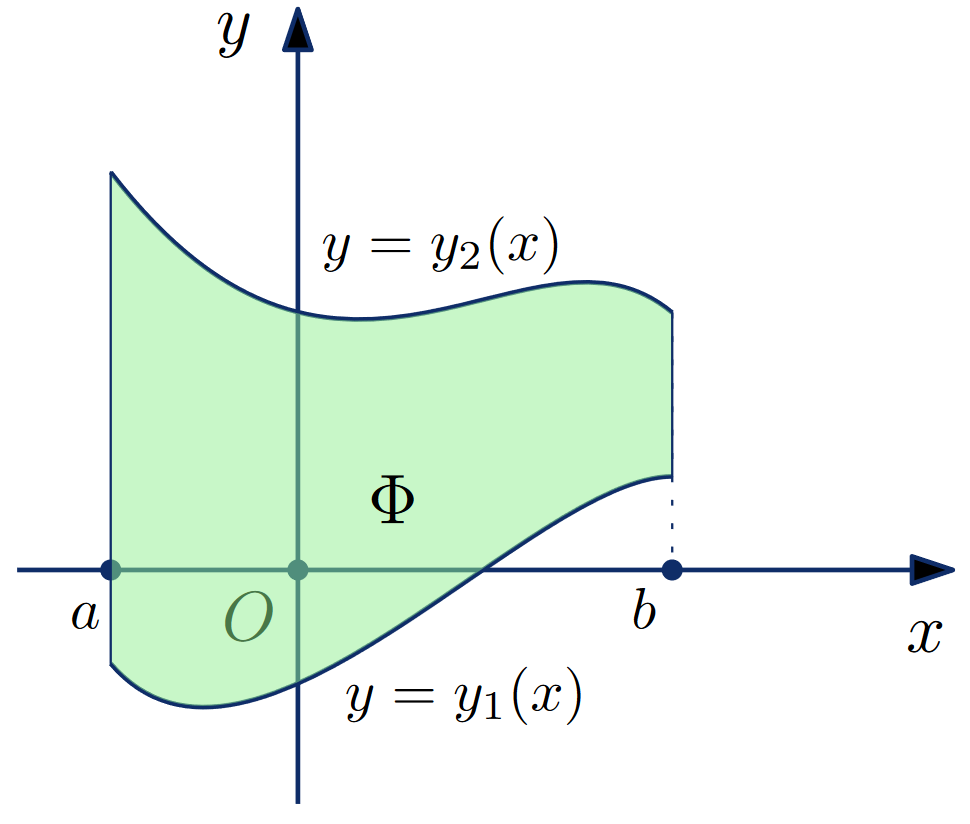
\includegraphics[width=0.3\textwidth]{img/lecture33/the_area_of_the_figure}
    \end{center}
    
    \begin{proof}
    	В предыдущем предложении мы рассматривали неотрицательные функции. Здесь мы можем функции $y_1(x)$ и $y_2(x)$ сдвинуть вверх на одну и ту же константу, таким образом, они станут неотрицательными, если не были таковыми до этого, приэтом искомая площадь останется неизменной.
    	
    	Знаем, что мера Жордана функции $y_2(x)$ - это интеграл $\int_a^b y_2(x) \; dx$, мера Жордана функции $y_1(x)$ - это интеграл $\int_a^b y_1(x) \; dx$. Получается, что мера Жордана искомой площади равна $\int_a^b y_2(x) \; dx - \int_a^b y_1(x) \; dx = \int_a^b (y_2(x) - y_1(x)) \; dx.$
    \end{proof}
    
    \section{Площадь в полярной системе координат}
    
    Полярная система координат — двумерная система координат, в которой каждая точка на плоскости определяется двумя числами — полярным углом и полярным радиусом. 
    
    \begin{center}
    	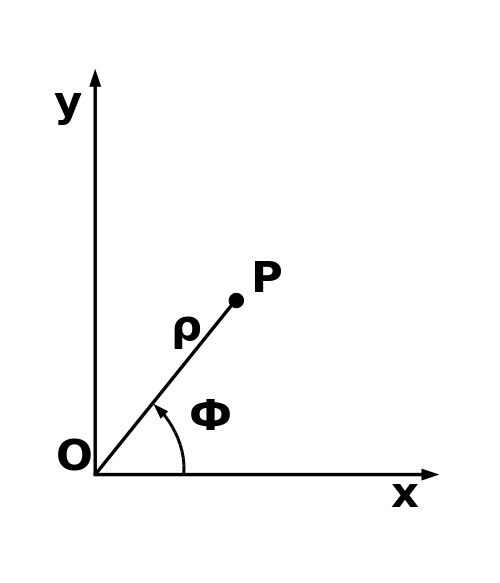
\includegraphics[width=0.3\textwidth]{img/lecture33/polar_coordinates}
    \end{center}
    
    Пару полярных координат $r$ и $\phi$ можно перевести в Декартовы координаты $x$ и $y$ путём применения тригонометрических функций синуса и косинуса
    \[ x = r\cos{\phi}, y = r\sin{\phi} \]
    Для $r$ = 0, $\phi$ может быть произвольным действительным числом. Для $r \neq 0$, чтобы получить уникальное значение $\phi$, следует ограничиться интервалом $[0, 2\pi)$.
    
    \begin{theorem}
    	Площадь сектора Ф, ограниченного графиком функции $r(\phi)$ в полярных
    	координатах и соответствующими
    	отрезками лучей $\phi = \alpha$ и $\phi = \beta$, равна
    	\[ S = \frac{1}{2} \int_{\alpha}^{\beta} r^2(\phi) \; d\phi. \]
    \end{theorem}
    
    \begin{center}
    	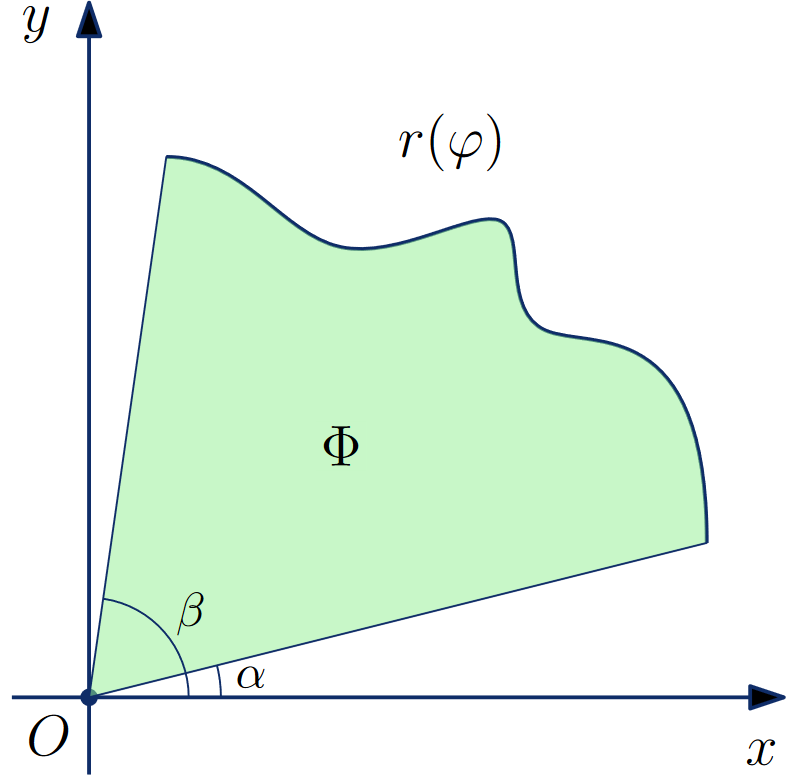
\includegraphics[width=0.2\textwidth]{img/lecture33/the_area_of_the_figure2}
    \end{center}
    
    \begin{proof}
    	Разделим фигуру на секторы, приэтом сначала выберем радиус сектора как минимальное расстояние до начал координат (красные секторы), а затем - как максимальное (зелёные секторы):
   	
   		\begin{center}
   			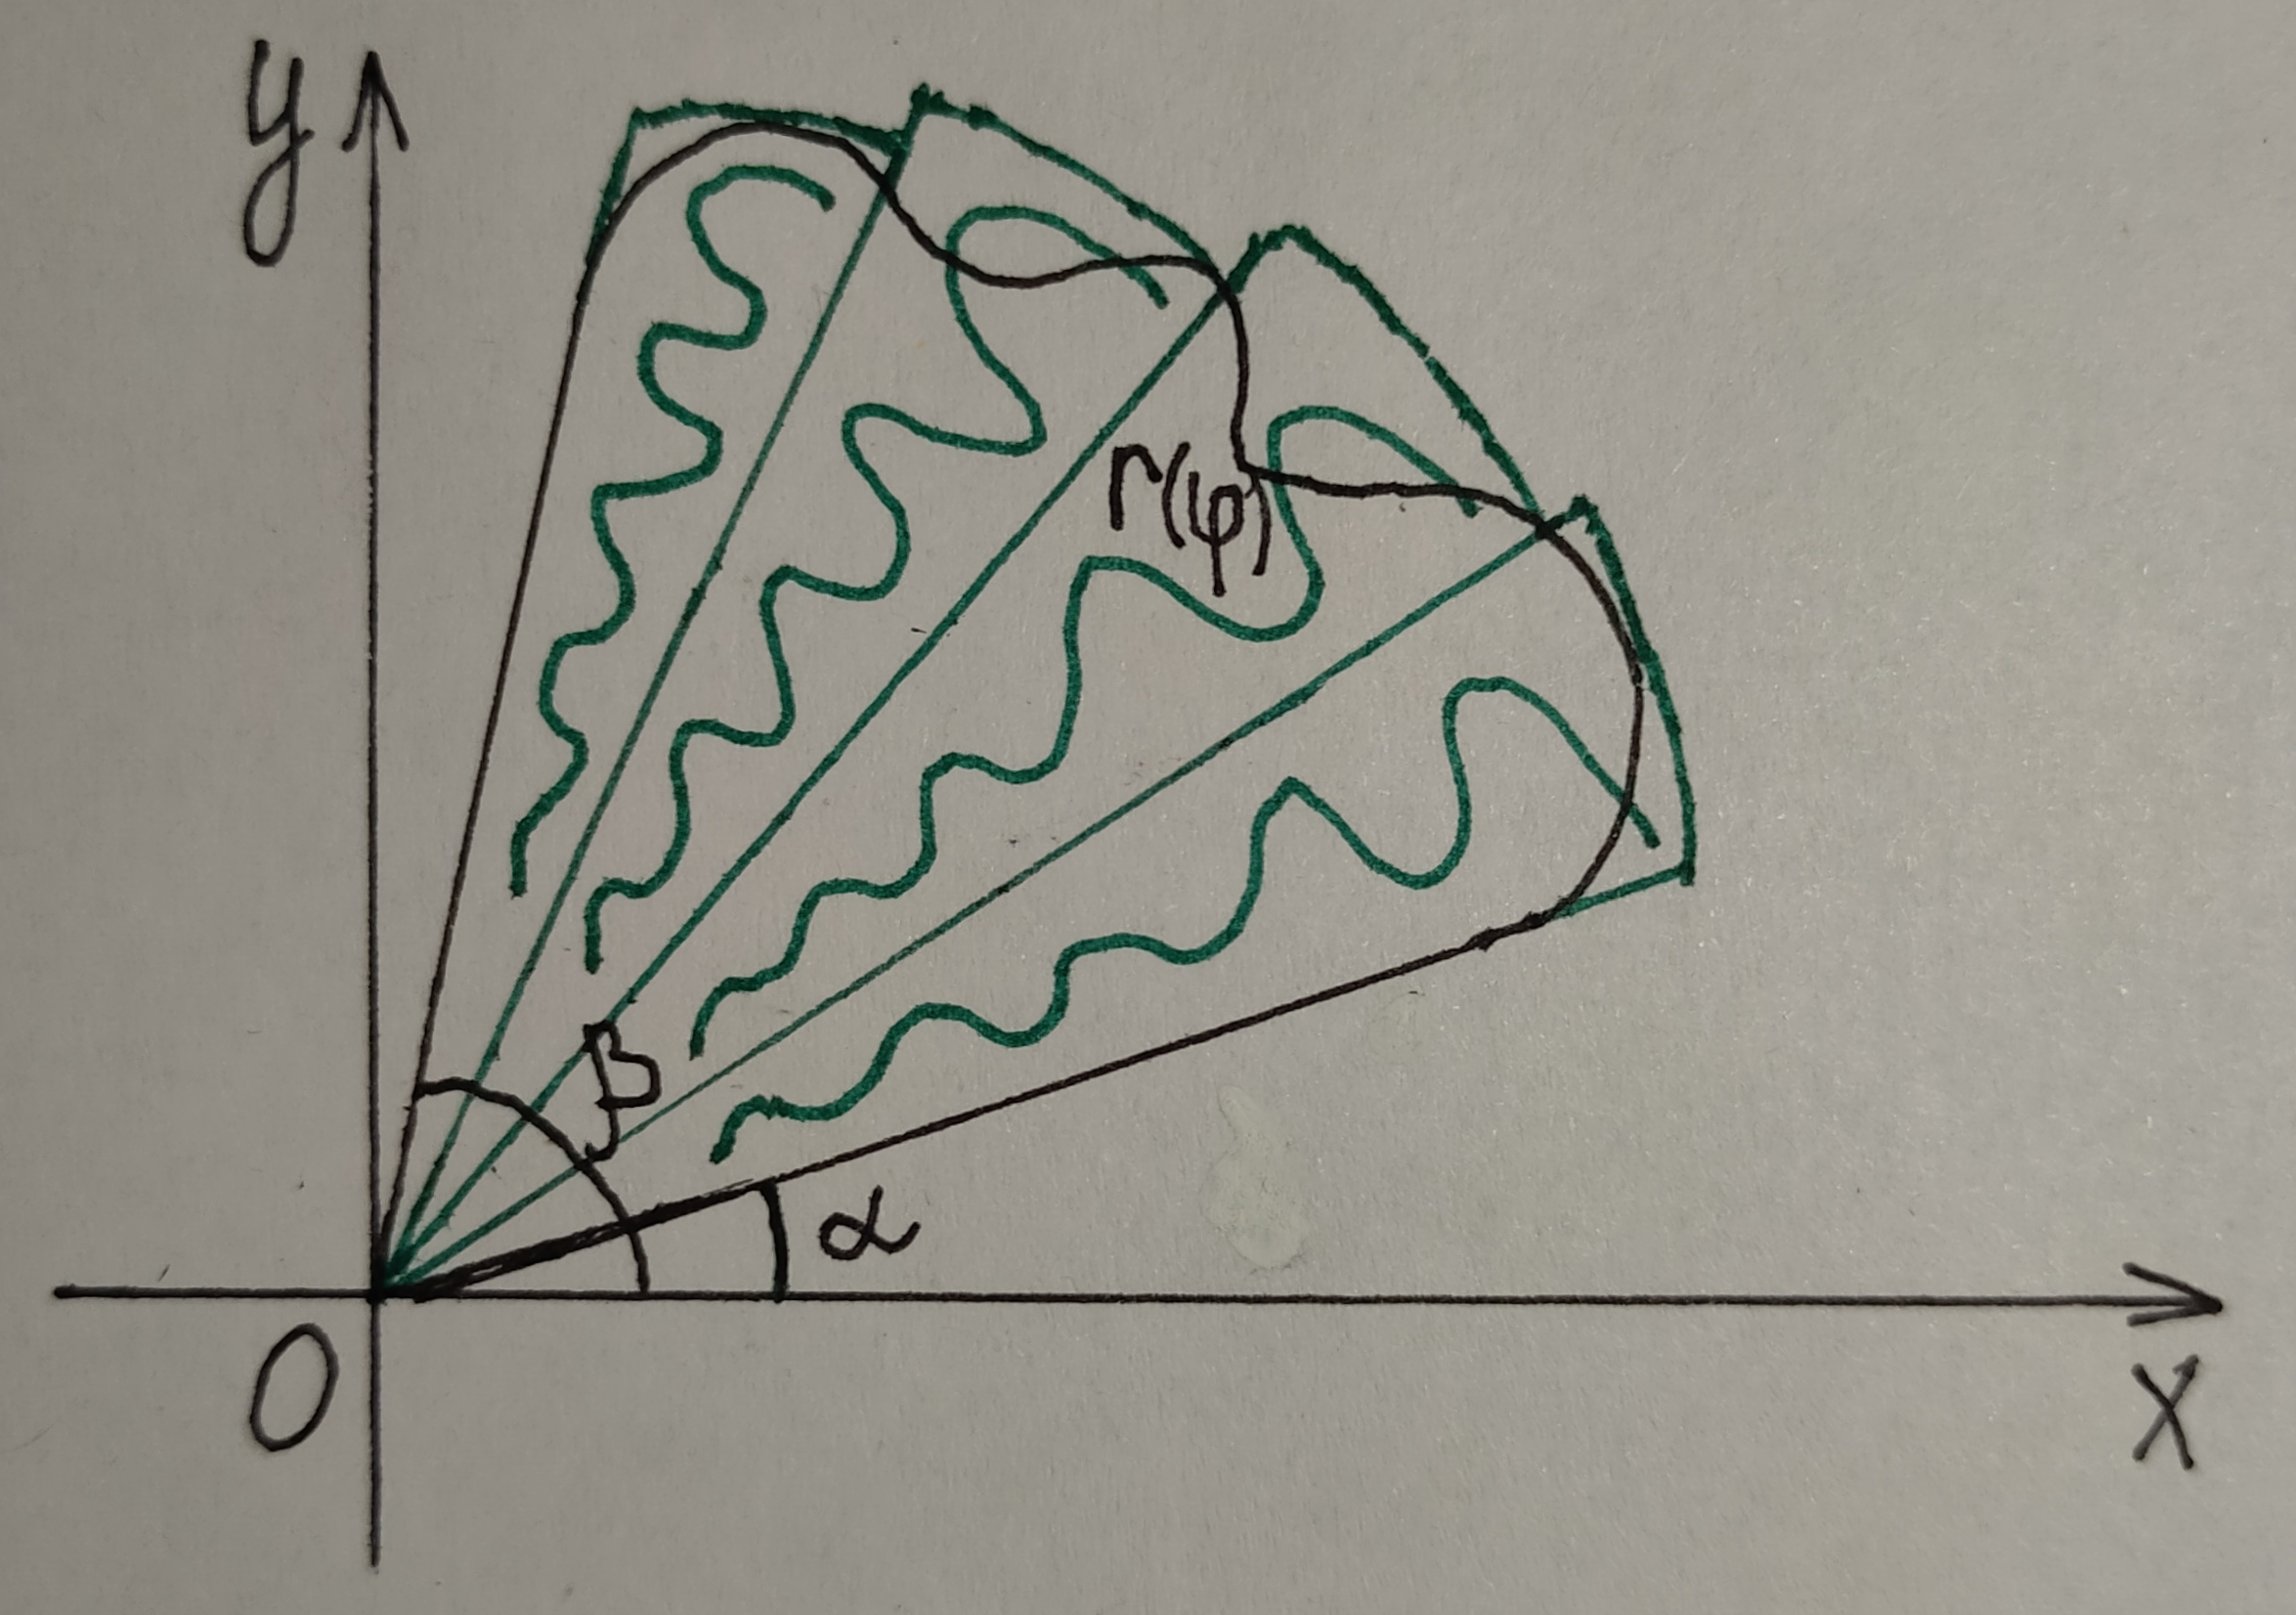
\includegraphics[width=0.3\textwidth]{img/lecture33/max_sectors}
   		\end{center}
   		\begin{center}
   		    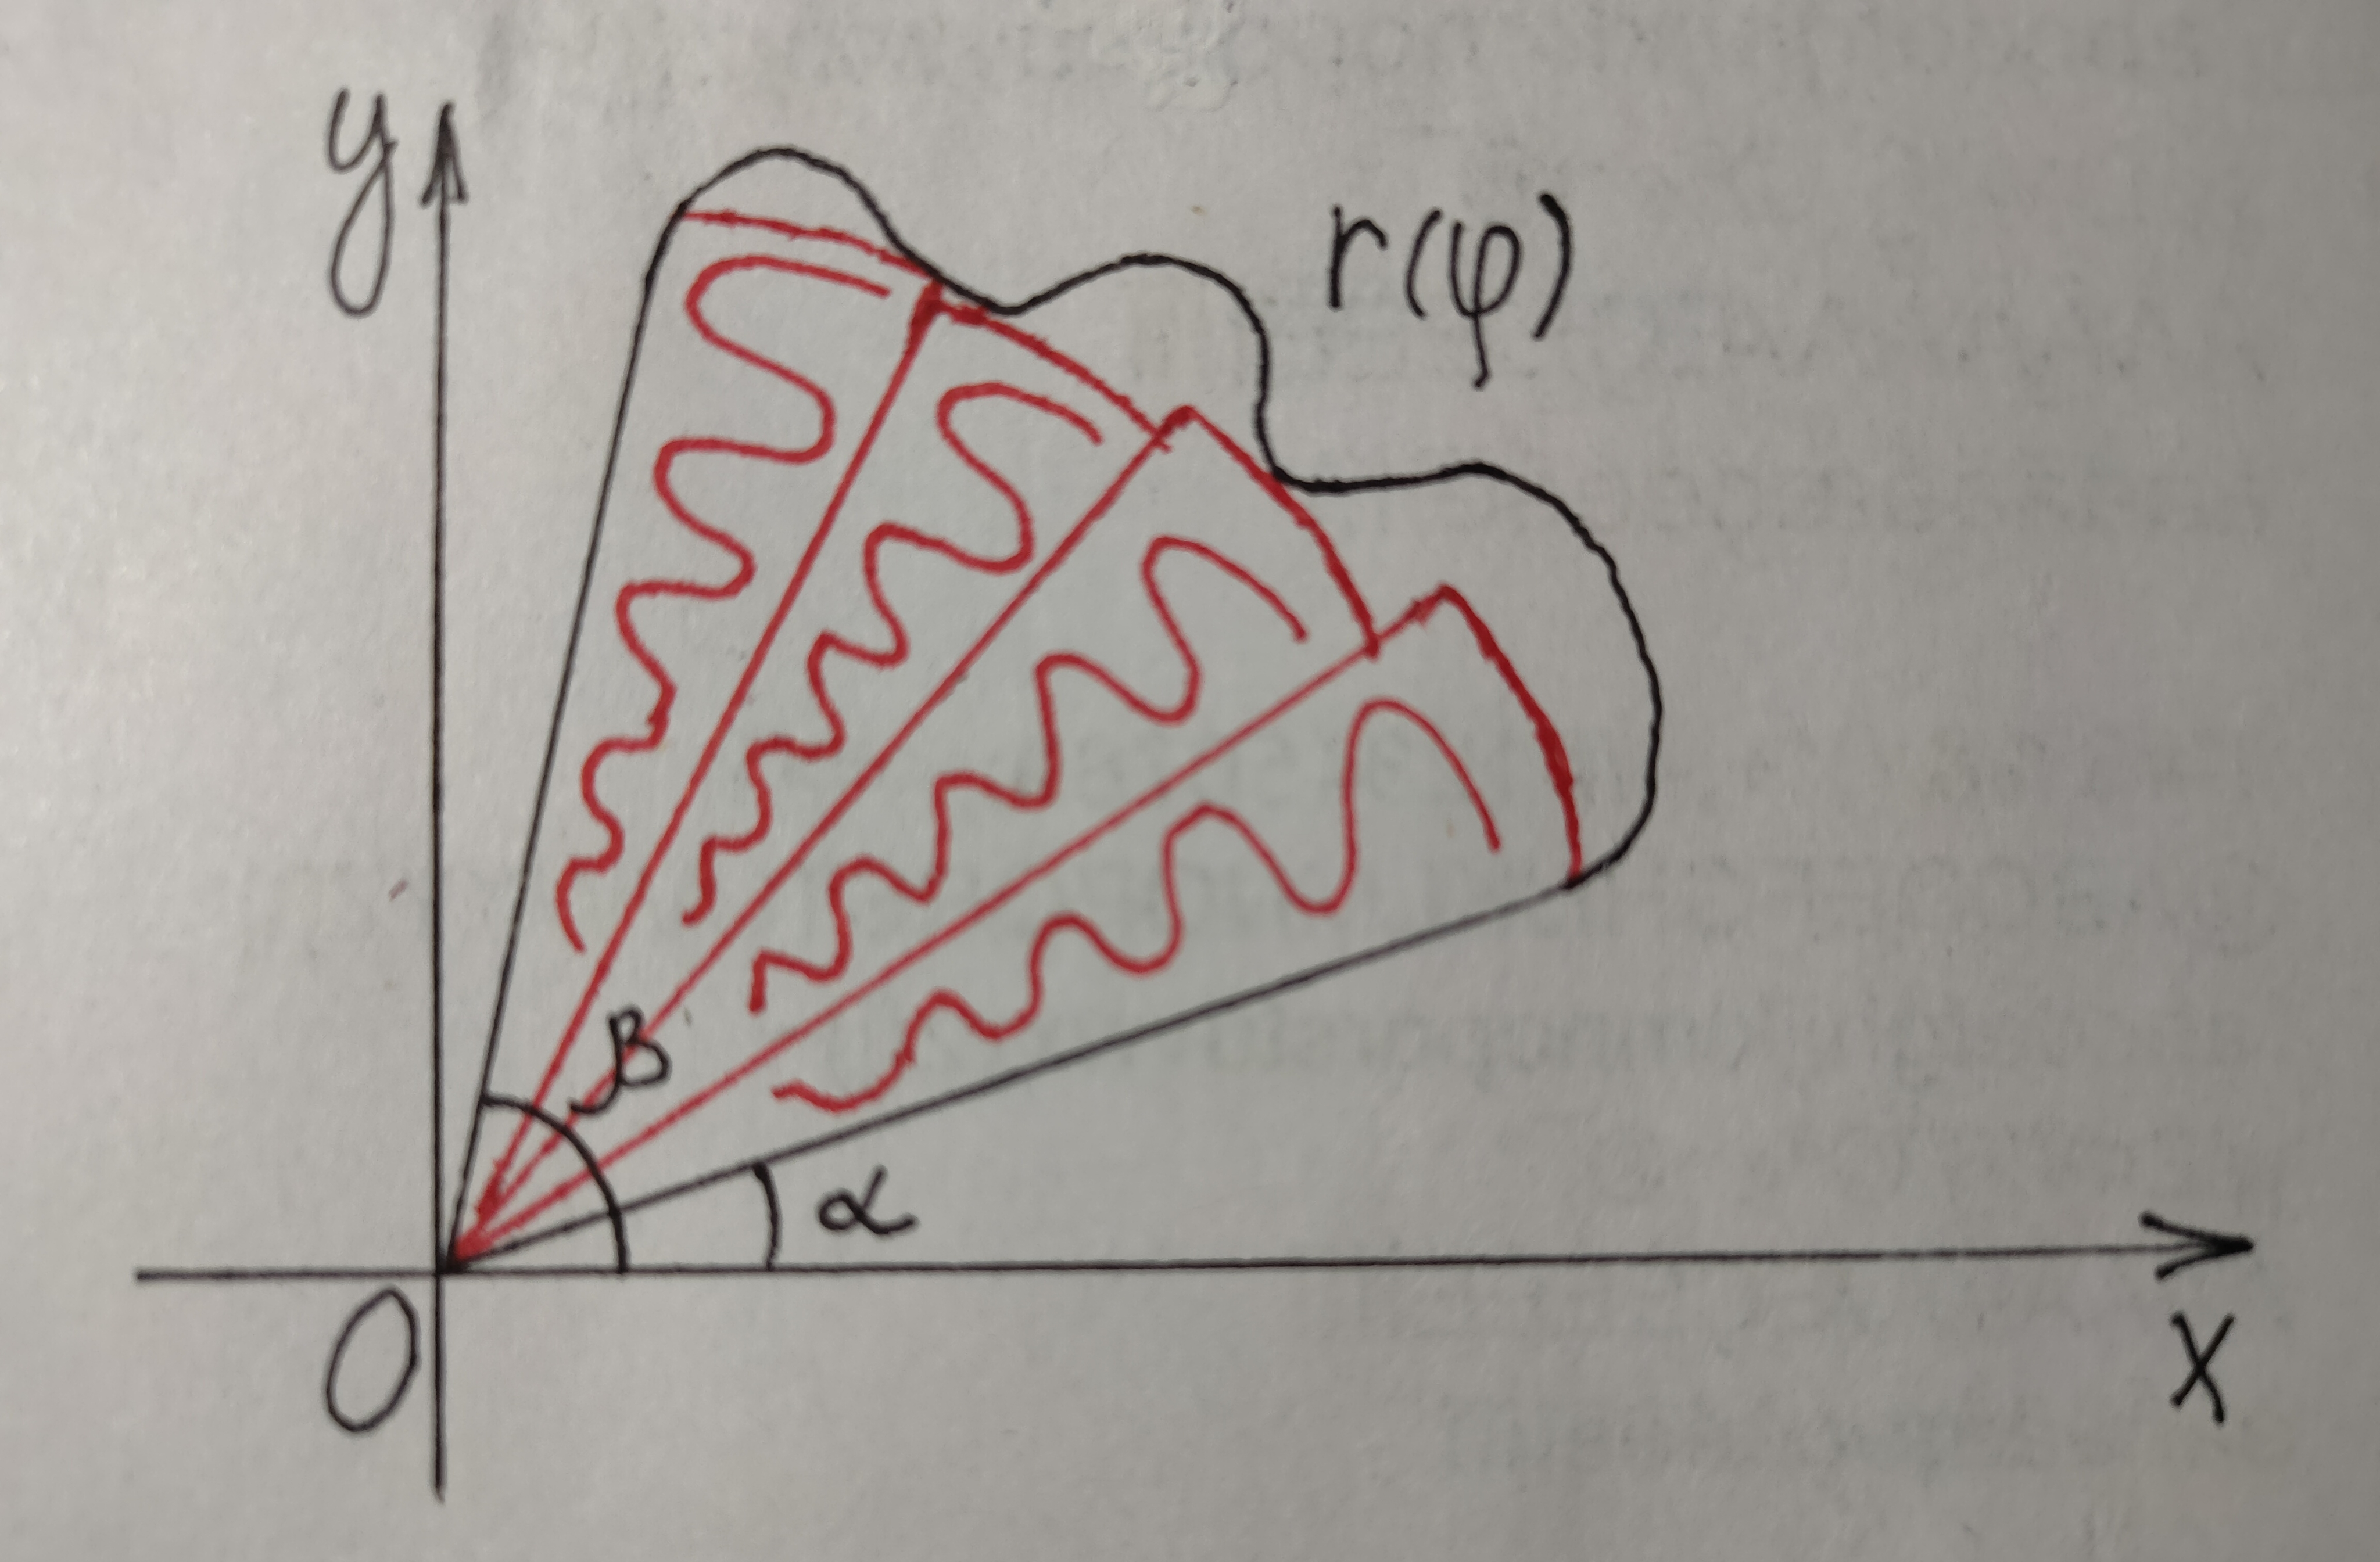
\includegraphics[width=0.3\textwidth]{img/lecture33/min_sectors}
   		\end{center}
   		
   		$T$ - разбиение $[\alpha, \beta]$
   		
   		Формулу площади круга $\pi r^2$ можно доказать, посчитав интеграл $4 \int_0^r \sqrt{r^2 - x^2} \; dx$ (фактически считаем площади четверти круга)
   		
   		\[ 4 \int_0^r \sqrt{r^2 - x^2} \; dx = 4 \int_0^r r\sqrt{1 - (\frac{x}{r})^2} \; dx = [\sin{\phi} = \frac{x}{r} \Rightarrow r\sin{\phi} = x \Rightarrow r\cos{\phi} d\phi = dx] = \] 
   		\[ = 4 \int_0^{\frac{\pi}{2}} r\sqrt{1 - \sin^2{\phi}} \cdot r \cos{\phi} \; d\phi = (*), \]
   		т. к. $\sin{\phi} = \frac{r}{r} = 1 \Rightarrow \phi = \frac{\pi}{2}, \sin{\phi} = \frac{0}{r} = 0 \Rightarrow \phi = 0.$
    	\[ (*) = 4 \int_0^{\frac{\pi}{2}} r \cos{\phi} \cdot r \cos{\phi} d\phi = 4 \int_0^{\frac{\pi}{2}} r^2 \cos^2{\phi} \; d\phi = 4r^2 \int_0^{\frac{\phi}{2}} \cos^2{\phi} \; d\phi = \] 
    	\[ = 4 r^2 \int_0^{\frac{\pi}{2}} \frac{1 + \cos{2\phi}}{2} \; d\phi = 2r^2 \int_0^{\frac{\pi}{2}} (1 + \cos{2\phi}) \; d\phi = 2r^2 \bigg(\phi + \frac{1}{2} \sin{2\phi} \bigg|_0^{\frac{\pi}{2}}\bigg) = \pi r^2 \]
    	
    	Тогда площадь сектора равна
    	\[ S_{(\phi_1, \phi_2)} = \frac{\pi r^2 (\phi_2 - \phi_1)}{2\pi} = \frac{r^2 (\phi_2 - \phi_1)}{2} \]
    	\begin{center}
    		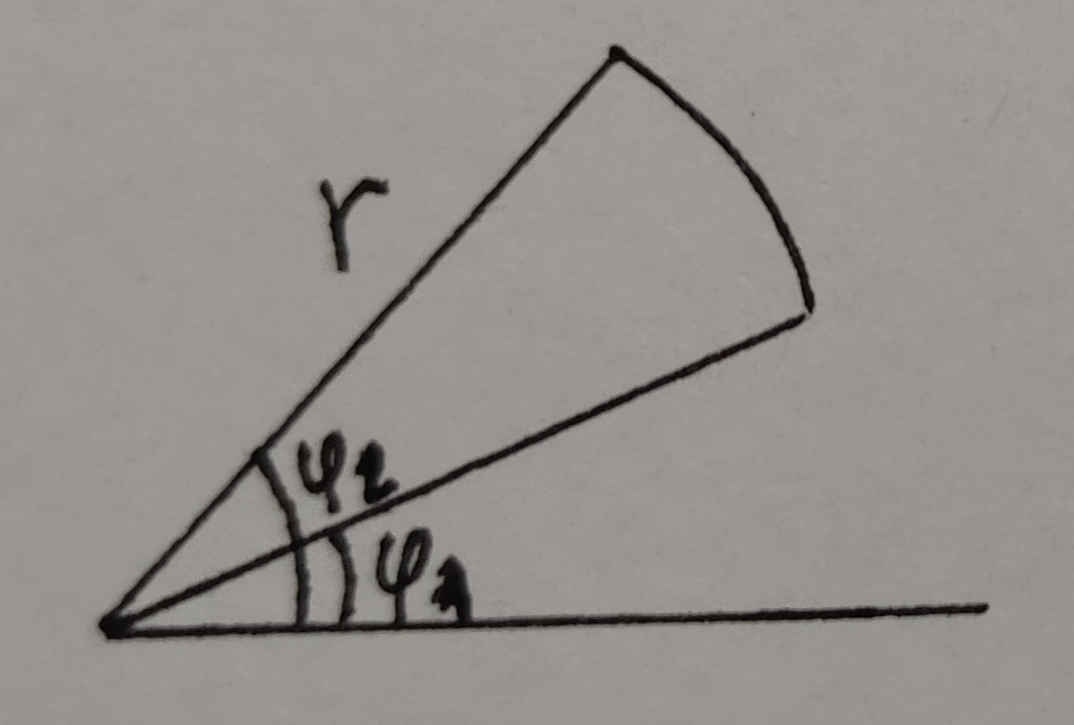
\includegraphics[width=0.2\textwidth]{img/lecture33/sector}
    	\end{center}
    	
    	Площадь красных секторов
    	\[ S_1 = \sum_{k = 1}^n \inf_{\phi \in \Delta_k} r^2(\phi) \frac{1}{2} \Delta\phi_k = s(g, T), \]
    	где $g(r) = \frac{r^2}{2}$, $\Delta\phi_k = \phi_k - \phi_{k - 1}$.
    	
    	Площадь зелёных секторов
    	\[ S_2 = \sum_{k = 1}^n \sup_{\phi \in \Delta_k} r^2(\phi) \frac{1}{2} \Delta\phi_k = S(g, T) \]
    	
    	$S(g, T)$ и $s(g, T)$ стремятся к интегралу. Мера Жордана зажата между ними $\Rightarrow$ тоже стремится к интегралу, т. е. к $\int_{\alpha}^{\beta} \frac{r^2(\phi)}{2} \; d\phi$.
    \end{proof}
    
    \begin{example}
    	На гиперболе $x^2 - y^2 = a^2$ дана точка $M(x_0; y_0)$. Найти площадь
    	криволинейного треугольника OAM. 
    \end{example}
    
    \begin{center}
    	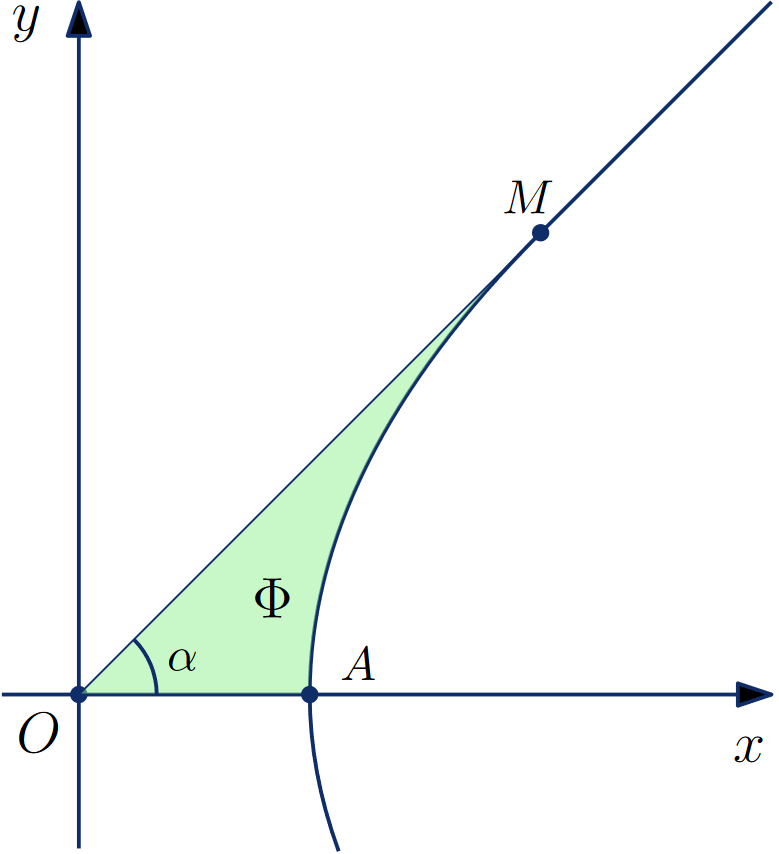
\includegraphics[width=0.2\textwidth]{img/lecture33/the_area_of_the_figure3}
    \end{center}
    
    Зададим в полярной системе координат гиперболу:
    \[ x^2 - y^2 = a^2 \Rightarrow r^2 \cos{\phi}^2 - r^2 \sin^2{\phi} = a^2 \Rightarrow r^2 (\cos{\phi}^2 - \sin{\phi}) = a^2 \Rightarrow r^2 = \frac{a^2}{\cos{2\phi}} \Rightarrow \]
    \[ \Rightarrow r = \frac{a}{\sqrt{\cos{2\phi}}} \]
    
    Угол точки $A$ равен 0, угол точки $M$ равен $\arctg{\frac{y_0}{x_0}}$.
    
    Осталось посчитать интеграл:
    \[ S = \frac{1}{2} \int_0^{\arctg{\frac{y_0}{x_0}}} \frac{a^2}{\cos{2\phi}} \; d\phi = \frac{a^2}{2} \int_0^{\arctg{\frac{y_0}{x_0}}} \frac{\cos{2\phi}}{\cos^2{2\phi}} \; d\phi = \frac{a^2}{4} \int_0^{\arctg{\frac{y_0}{x_0}}} \frac{d\sin{2\phi}}{\cos^2{2\phi}} = \]
    \[ = \frac{a^2}{4} \int_0^{\arctg{\frac{y_0}{x_0}}} \frac{d\sin{2\phi}}{1 - \sin^2{2\phi}} = \frac{a^2}{8} \ln{\bigg|\frac{1 - \sin{2\arctg{\frac{y_0}{x_0}}}}{1 + \sin{2\arctg{\frac{y_0}{x_0}}}}\bigg|} + C = (*) \]
    В силу формулы $\sin{\alpha} = \frac{2\tg{\frac{\alpha}{2}}}{1 + \tg^2{\frac{\alpha}{2}}}$ получаем, что
    \[ (*) = \frac{a^2}{8} \ln{\bigg|\frac{1 - \frac{2 \frac{y_0}{x_0}}{1 + \frac{y_0^2}{x_0^2}}}{1 + \frac{2 \frac{y_0}{x_0}}{1 + \frac{y_0^2}{x_0^2}}}\bigg|} + C \]
    
    \section{Объем тел вращения}
    
    \begin{theorem}
    	Пусть функция $y = y(x)$ непрерывна и неотрицательна на отрезке $[a; b]$. Объем $V$ тела, образованного вращением вокруг оси Ox фигуры Ф, ограниченной графиком функции $f(x)$, отрезками прямых $x = a$ и $x = b$ и отрезком оси $Ox$, равен
    	\[ V = \pi \int_a^b f^2(x) \; dx. \]
    \end{theorem}
    
    \begin{center}
    	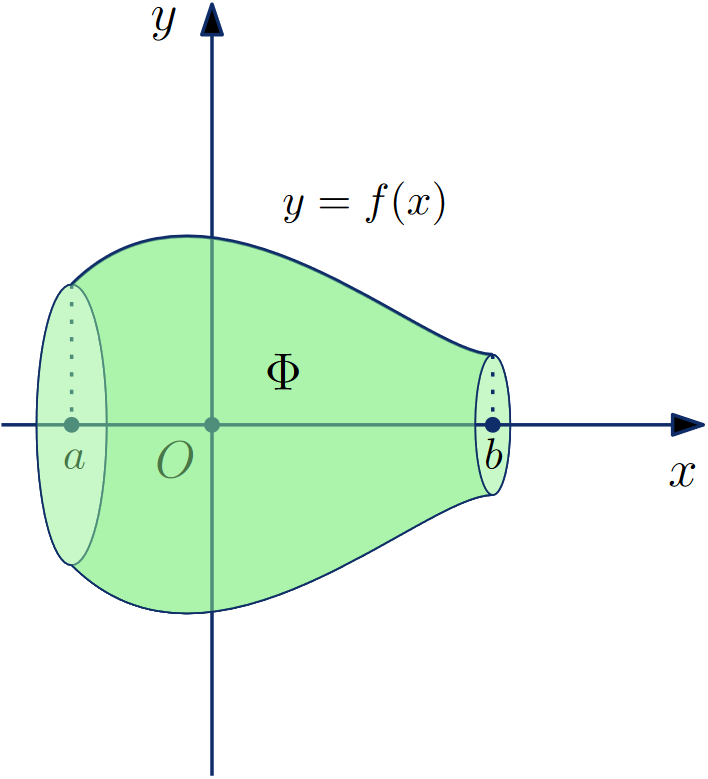
\includegraphics[width=0.3\textwidth]{img/lecture33/the_area_of_the_figure4}
    \end{center}
    
    \begin{proof}
    	Обозначим через $G$ тело, образованное вращением вокруг оси $Ox$ фигуры Ф. Рассмотрим разбиение $T = \{x_0, x_1, ..., x_n\}$ отрезка $[a; b]$. Заметим, что фигура $C_1(T)$, состоящая из цилиндров высоты $h_k = x_k - x_{k - 1}$ радиуса $R = \sup_{x \in \Delta_k} f(x)$, покрывает тело вращения $G$. А фигура $C_2(T)$, состоящая из цилиндров высоты $h_k = x_k - x_{k - 1}$ радиуса $R = \inf_{x \in \Delta_k} f(x)$, наоборот, вписана в тело вращения $G$. Как известно, объем цилиндра радиуса $R$ и высоты $h$ равен $\pi R^2 h$. Отсюда получаем, что
    	\[ \mu(C_2(T)) = \sum_{k = 1}^n \pi \inf_{x \in \Delta_k} f^2(x) \Delta x_k \leqslant \sum_{k = 1}^n \pi \sup_{x \in \Delta_k} f^2(x) \Delta x_k = \mu(C_1(T)). \]
    	В правом и левой частях неравенства стоят в точности нижняя и верхняя суммы Дарбу для функции $\pi f^2(x)$. Поскольку функция $f(x)$ непрерывна, она является интегрируемой (следствие 10.13). А значит интегрируем и ее квадрат (следствие 10.7). Тем самым получаем, что
    	\[ \mu(C_1(T)), \mu(C_2(T)) \to I = \pi \int_a^b f^2(x) \; dx \text{ при } \Delta_T \to 0. \]
    	Это означает, что $G$ измеримо по Жордану, и его объем равен $V = \pi \int_a^b f^2(x) \; dx$.
    \end{proof}
    
    \begin{example}
    	Найти объем тела, образованного при вращении круга $(x - a)^2 + y^2 \leqslant a^2$ вокруг оси Oy.
    \end{example}
    
    \begin{theorem}
    	Пусть в полуплоскости $y \geqslant 0$ параметрически задана кривая уравнениями
    	\[ x(t), y(t), t \in [\alpha; \beta], \]
    	где $x(t)$ и $y(t)$ — непрерывно дифференцируемые на $[a; b]$ функции. Площадь $S$ поверхности, образованной при вращении данной кривой вокруг оси $Ox$, равна
    	\[ S = 2\pi \int_{\alpha}^{\beta} y(t) \sqrt{x'^2(t) + y'^2(t)} \; dt. \]
    \end{theorem}
    
    \begin{theorem}
    	Пусть $y = y(x)$ - непрерывно дифференцируемая на отрезке $[a; b]$ функция.
    	Площадь $S$ поверхности, образованной при вращении графика этой функции вокруг оси $Ox$, равна
    	\[ S = 2\pi \int_a^b |y(x)|\sqrt{1 + y'^2(x)} \; dx. \]
    \end{theorem}
    
    \begin{example}
        Найти площадь поверхности, образованной при вращении эллипса $x^2 + 4y^2 = 36$ вокруг оси $Oy$.
    \end{example}
    
    \section{Длина кривой}
    
    \begin{definition}
    	Пусть $\gamma : [a, b] \rightarrow \R^3$ - гладкая кривая, т.е. $\gamma(t) = (x(t), y(t), z(t))$ и функции $x, y, z \in C^1([a, b])$. Пусть $\ell(a, b)$ — длина пути соответствующая отрезку $[a, b]$. Тогда длина кривой удовлетворяет следующим требованиям
        \begin{enumerate}
        	\item $\ell(\alpha, \gamma) = \ell(\alpha, \beta) + \ell(\beta, \gamma)$ при $a \leqslant \alpha < \beta < \gamma \leqslant b$;
        	\item $\inf_{t \in [\alpha, \beta]} |v(t)|(\beta - \alpha) < \ell(\alpha, \beta) \leqslant \sup_{t \in [\alpha, \beta]} |v(t)|(\beta - \alpha)$, где $v(t) = (x'(t), y'(t), z'(t))$.
        \end{enumerate}
    \end{definition}
    
    \begin{theorem}
    	Длина кривой, заданной параметрически уравнениями
    	\[ x = x(t), y = y(t), z = z(t), t \in [a; b], \]
    	где $x(t), y(t), z(t)$ — непрерывно дифференцируемые на $[a; b]$ функции, равна
    	\[ s = \int_a^b \sqrt{x'^2 + y'^2 + z'^2} \; dx \]
    \end{theorem}
	
\end{document}
